% \documentclass[draft]{article}
% \usepackage[utf8]{inputenc}
% \usepackage{graphicx}
% \usepackage{tikz}
% \usepackage{etex}
% \usepackage{pgfplots}
% \usepackage{pgf,pgfsys,pgffor}
% \usepackage[utf8]{inputenc}
% \usepackage{graphicx}% Include figure files
% \graphicspath{ {images/} }
% \usepackage[rightcaption]{sidecap}
% \let\olditemize\itemize
% \def\itemize{\olditemize\itemsep=1pt }
% \usepackage{wrapfig}
% \usepackage{dcolumn}% Align table columns on decimal point 
% \usepackage{comment}
% \usepackage{bm}% bold math
% %\usepackage[mathlines]{ineno}%\titlespacing*{\section}{0pt}{1.1\baselineskip}{\baselineskip} Enable numbering of text and display math
% %\linenumbers\relax % Commence numbering line
% \usepackage{cancel}
% \usepackage{amsmath}
% \usepackage{wrapfig}
% \usepackage{subfigure}
% \usepackage{amssymb}
% \usepackage{mathrsfs}
% \newcommand{\angstrom}{\textup{\AA}}
% \usepackage{enumerate}
% \usepackage{vmargin}
% \usepackage{setspace}
% \usepackage{hyperref}
% \usepackage{enumitem}
% \usepackage{longtable}
% \usepackage{multirow}
% \usepackage{caption}
% % Set link colors
% \hypersetup{colorlinks, breaklinks, urlcolor=red, linkcolor=blue, citecolor=cyan}
% \usepackage{natbib}
% \bibliographystyle{plainnat}

% \pgfplotsset{compat=1.14}
% \setpapersize{A4}
% \setmargins{2.5cm}       % margen izquierdo
% {1.5cm}                        % margen superior
% {16.5cm}                      % anchura del texto
% {23.42cm}                    % altura del texto
% {12pt}                           % altura de los encabezados
% {1.5cm}                           % espacio entre el texto y los encabezados
% {0pt}                             % altura del pie de página
% {2cm}                           % espacio entre el texto y el pie de página
% \title{article}
% \author{}
% \date{February 2019}


%                                                                 aa.dem
% AA vers. 8.2, LaTeX class for Astronomy & Astrophysics
% demonstration file
%                                                       (c) EDP Sciences
%-----------------------------------------------------------------------
%
%\documentclass[referee]{aa} % for a referee version
%\documentclass[onecolumn]{aa} % for a paper on 1 column  
%\documentclass[longauth]{aa} % for the long lists of affiliations 
%\documentclass[rnote]{aa} % for the research notes
%\documentclass[letter]{aa} % for the letters 
%\documentclass[bibyear]{aa} % if the references are not structured 
% according to the author-year natbib style
%
% \documentclass[draft]{aa}
\documentclass{aa}
%
\usepackage{graphicx}
\usepackage{txfonts}
\usepackage{natbib}
\usepackage[]{hyperref}
\hypersetup{colorlinks=true, urlcolor=blue, citecolor=cyan, pdfborder={0 0 0},}

% Ignore Appendix
% \renewcommand\appendix{\end{document}}

% "Fix" hyperlink spilling out of page error
% \hypersetup{draft}

\begin{document}

% \section*{Abstract}
% 

 \title{Title in progress}

% \subtitle{I. Overviewing the $\kappa$-mechanism}

\author{G. I. Perren\inst{1,2}
      \and
      E. E. Giorgi\inst{1}
      \and
      A. Moitinho\inst{3}
      \and
      G. Carraro\inst{4}
      \and
      M. S. Pera\inst{2}
      \and
      R. A. Vázquez\inst{1,2}
      % \fnmsep\thanks{Just to show the usage
      % of the elements in the author field}
}

\institute{Facultad de Ciencias Astronómicas y Geofísicas (UNLP),
IALP-CONICET, 1900 La Plata, Argentina\\
\email{gabrielperren@gmail.com}
\and
Consejo Nacional de Investigaciones Científicas y Técnicas (CONICET), Buenos
Aires, Argentina
\and
SIM, Faculdade de Ciências, Universidade de Lisboa, Ed. C8, Campo Grande,
P-1749-016 Lisboa, Portugal
\and
Dipartimento di Fisica Astronomia Galileo Galilei, Vicolo Osservatorio 3,
Padova, I-35122, Italy
% \thanks{The university of heaven temporarily does not
%         accept e-mails}
}

\date{Received June 15, 2019; accepted September 16, 2019}

\abstract{ 
% 5 {} token are mandatory
We have carried out an \textit{UBVI} photometric study on sixteen faint and
unknown open clusters placed along the Milky Way plane in a sector extending
from $290^\circ$ to $320^\circ$ in galactic longitude. The photometric
observations were analyzed -for the most part- in an automatic way in order to
get a homogeneous set of results regarding distance, reddening, mass, age and
metallicity for each individual cluster. Distances obtained from the photometric
analysis were then compared using the GAIA satellite $2^{nd}$ data release (GAIA
DR2), parallax and proper motions, trough a Bayesian analysis.
%
We have found that only eight out of the sixteen clusters are real entities and
another two remain categorized as probable open clusters. The rest of them in
the sample are most probably random stellar fluctuations. The comparison of
distances coming from the photometric analysis and from GAIA data for these ten
clusters has yielded a variable level of disagreement.
%
Indeed since most of GAIA our real clusters are at distance larger than 1.9 kpc,
our distances from photometry and the ones obtained via GAIA are not entirely
coincident given the uncertainties in parallaxes for distant objects up to now,
even applying the suggested systematic zero point correction for parallax from
recent literature.
%
We draw attention to the importance use in this article of the \textit{U-B}
index which allows us to perform a realistic estimate of the reddening for each
cluster and therefore of the visual absorption, which is a critical parameter for
obtaining a more accurate distance determination when using photometric methods.
%
In this sense we found that in the case of robust open clusters such as NGC 4349
and Trumpler 13 distances from both methods tend to be coincident. As for the
contribution of the present sample to the knowledge of the spiral structure
nearby to the Sun, we found just three objects which are young enough as to be
assumed potential spiral arm components located not far from the Carina feature.
}{}{}{}{}

\keywords{giant planet formation --
              $\kappa$-mechanism --
              stability of gas spheres
             }

\maketitle




%================================================================
\section{Introduction}

Galactic open clusters are routinely used as probes of the structure and
evolution of the Milky Way disk. Their fundamental parameters, like age,
distance, and metallicity allow us to define the large scale structure of the
disk and to cast light on its origin and assembly \citep{Janes_1982,
2018A&A...618A..93C}. Young open clusters can be used to trace spiral
arms and star forming regions \citep{Vazquez2008}, while older clusters are
better probes of the chemical evolution of the thin disk
\citep{2009yCat..35120063M}. The recent second release of Gaia satellite data
\citep{GaiaDR2_2018} is producing a tremendous advance in the study of the
Galactic disk and its star cluster population.

Basic parameters for a large number of clusters are now available with
unprecedented accuracy \citep{2018A&A...618A..93C}. Proper motions may be
employed to select cluster members and parallaxes can be used to derive
distances. It comes to happen that in some cases Gaia based distances strongly
disagree with photometric or spectrophotometric distances. Nonetheless, for
reasonably short distances the two different methods yield similar results
within the uncertainties \citep{2018A&A...618A..93C}. At larger distances Gaia
photometry is of poorer quality than the more traditional ground based
photometry, and accurate parallaxes are not available or possible for the
moment. It is difficult to say which the critical distance is, since it also
depends on the interstellar absorption and the crowding of a given star cluster.
In all cases it is necessary to count on cleaner color-color and color-magnitude
diagrams.

In this work we put together a sample of previously unstudied star clusters
located at different distances for which we provide CCD \textit{UBVI}
photometry, and complement with data available from Gaia DR2. The purpose of
this investigation is twofold. Firstly, we wanted to study Galactic structure in
a poorly known Galactic sector, located at approximately $270^\circ < l <
300^\circ$. In this region one would expect to be able to follow the Perseus arm
coming out of the third Galactic quadrant. On the contrary, no stellar traces
have been detected so far for this arm, which is so prominent in the second
quadrant, and clearly visible also in the third. The sample of clusters
originally selected for this purpose and analyzed in this paper is shown in
Table 1 together with their absolute coordinates referred to the J2000.0 equinox
and also the galactic ones. However, this proved quite a difficult task, since
in that specific sector extinction is particularly strong, and variable. This
makes it cumbersome not only to derive solid basic parameters, but, even worse,
to establish if a visual stellar aggregate is a physical cluster or simply a
random enhancement of field stars produced by patchy reddening.
Secondly, Gaia DR2 offers us a possible way out. On one side, in fact, we can
use Gaia data to make our analysis more robust for those clusters for which
\textit{UBVI} CCD data and Gaia DR2 counterparts are available. On the other
side, for the most distant clusters we are forced to use only our data, but with
the confidence that for shorter distances our method should provide identical
results as Gaia. For these reasons we employed the Automated Stellar
Cluster Analysis code \citep[\texttt{ASteCA};][]{Perren_2015} to derive
clusters' fundamental parameters from \textit{UBVI} data, and a Bayesian
technique to extract membership and distances from Gaia DR2.\\

The layout of the paper is as follows: in Section \ref{sec:clust_sample} we
present the cluster sample indicating their positions in the Galaxy.
Section \ref{sec:photo_obs} is devoted to explain the observations and the
reduction process of photometry. In Section \ref{sec:photom_analysis} we
describe the tools to analyze the photometric data and the method to connect
Gaia DR2 with photometric results. A cluster by cluster report of the results
obtained is presented in Section \ref{sec:cluster_discuss}.
Conclusions of the paper are given in Section \ref{sec:results_concl}.




%================================================================
\section{The cluster sample}
\label{sec:clust_sample}

Table \ref{tab:clust_list} shows equatorial coordinates ($\alpha$, $\delta$) and
galactic coordinates (\textit{l}, \textit{b}) for the clusters in the present
sample, ordered by increasing right ascension $\alpha$. Equatorial coordinates
refer to the J2000.0 equinox.

\begin{table}[ht]
    \centering
    \begin{tabular}{lcccc}
    \hline 
        Cluster name & $\alpha_{2000}$ & $\delta_{2000}$ & \emph{l} & \emph{b}\\
         & hh:mm:ss & dd:mm:ss & $^\circ$ & $^\circ$\\
       \hline \hline 
        vdBH 73 & 09:31:56 & -50:13:00 & 273.634 & 0.951\\
        RUP 85 & 10:01:33 & -55:01:12 &280.150 & 0.160\\
        vdBH 85 & 10:01:52 & -49:34:00 & 276.914 & 4.544\\
        vdBH 87 & 10:04:18 & -55:26:00 & 280.719 & 0.059\\
        TR 12 & 10:06:29 & -60:18:00 & 283.828 & -3698\\
        RUP 87 & 10:15:32 & -50:43:00 & 279.372 & 4.883\\
        vdBH91 & 10:17:16 & -58:42:00 & 284.030 & -1.600\\
        RUP 88 & 10:18:55 & -63:08:00 & 286.661 & -5.186\\
        vdHB92 & 10:19:07 & -56:25:00 & 282.984 & 0.438\\
        TR 13 & 10:23:48 & -60:08:00 & 285.515 & -2.353\\
        vdBH 106 & 10:52:42 & -54:14:00 & 286.048 & 4.700\\
        RUP 162 & 10:52:54 & -62:19:00 & 289.638 & -2.545\\
        Lynga 15 & 11:42:24 & -62:29:00 & 295.053 & -0.672\\
        Loden 565 & 12:08:06 & -60:43:12 & 297.650 & 1.710\\
        NGC 4230 & 12:17:20 & -55:06:06 & 298.025 & 7.445\\
        NGC 4349 & 12:24:08 & -61:52:18 & 299.719 & 0.830\\
        \hline
    \end{tabular}
    \caption{List of objects surveyed in the present article.
    Note: \textit{For the sake of saving space we indicate van den Bergh-Hagen
    clusters using the vdBH abbreviations all along the text. In a similar
    way Ruprecht and Trumpler clusters are mentioned as RUP and TR followed
    by the respective numbers.}}
    \label{tab:clust_list}
\end{table}

Positions of the clusters in the Galaxy are shown in Fig. \ref{fig1} superposed
onto the Aladin Sky Atlas DSS2 color image. Our sampling chiefly covers the
region around Carina OB association and the south-east part of Vela with some
objects in Crux and Centaurus.

\begin{figure*}[ht]
    \centering
    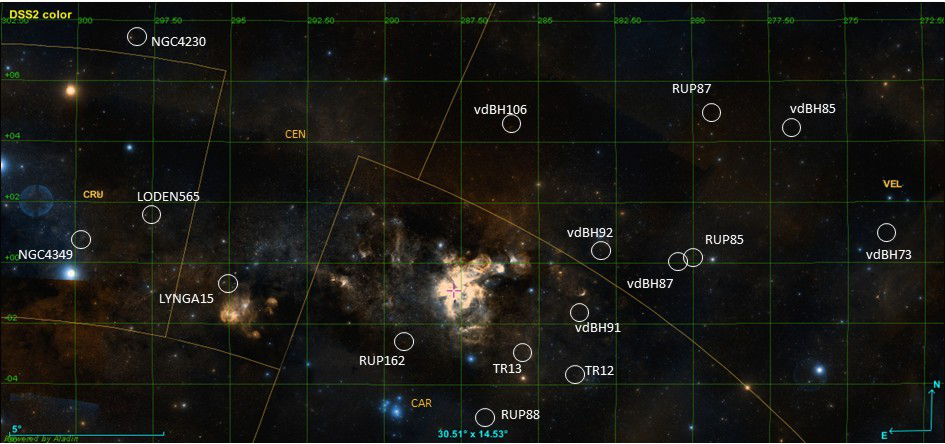
\includegraphics[width=\hsize]{figs/high_res/DSS2color.png}
    \caption{DSS2 color Aladin image showing with white circles the position of
    the clusters surveyed in the present sample. The galactic coordinates $l$
    and $b$ are depicted by a green grid while constellation limits for Carina,
    Vela, Centaurus and Crux appear in yellow lines.}
    \label{fig1}
\end{figure*}




%================================================================
\section{Photometric observations}
\label{sec:photo_obs}

A first series of CCD \emph{UBVI} photometry was carried out in 13 open clusters
placed in the galactic region going from 280$^\circ$ to 300$^\circ$ in galactic
longitude and from 7$^\circ$ to -5$^\circ$ in galactic latitude. This region
covers the Carina Arm, the inter-arm region between the Perseus and Carina arms
and also a part of the Local Arm.
Observations were made using the YALO facilities at Cerro Tololo Inter-american
Observatory on 9 nights in April and May 2002. Images were taken with a
$2048\times2048$ Tek CCD attached to the 90-cm telescope and the standard set of
\textit{UBVI} filters available at CTIO. The 0.39 arcsec/px plate scale
resulted in a field of view of $13\times13$ arcmins. Images were acquired using
the CTIO ARCON operating in Quad
mode\footnote{\url{http://www.ctio.noao.edu/instruments/arcon/arcon.html}}. The
CCD gain was set at 3.2 e$^-$/adu and the readout noise was determined to be 4.0
e$^-$.

A second series of CCD photometry was implemented during 2 nights (February and
March 2010) at Cerro Tololo Interamerican Observatory to get \textit{UBVI}
photometry in two other clusters, NGC 4349 and Lynga 15, at a slightly larger
galactic longitude (298$^\circ$). Images in a first run were taken with the CTIO
0.9 m telescope using a $2048\times2046$ px detector with a scale 0.401”/px
covering thus 13.6 arcmin on a side. A second run of images taken at the 1.0 m
telescope of the same clusters was carried out with a $4064\times4064$ px CCD
with a scale of $0.289$ arcsec/px thus covering $20\prime\times20\prime$ on a
side.
%
The first run (at the 0.9 m) was not photometric, and therefore we tied all
the images to the second night (at the 1.0 m), which was photometric. During
this second night, we took multiple images of the standard star fields PG 1047
and SA98 \citep{1992AJ....104..340L}, covering an air mass range $1.15-2.2$.

Details of exposure times per filter and telescope can be seen in Tables
\ref{tab:log_yalo} and \ref{tab:log_ctio} for the first and second series respectively.\\


\begin{table*}[ht]
    \centering
    \begin{tabular}{lcccccc}
    \hline 
        Cluster & Date &  &  & Pass band &  & \\
        &  & U & B & V & R & I\\
        Exp. Times (secs) &  & long/short & long/short & long/short & long/short & long/short\\
       \hline \hline 
        RUP 85 & 04/04/2002 & 300/30 & 200/5 & 160/3 & 160/2 & 120/1\\
        vdBH 85 & 04/05/2002 & 300/30 & 200/5 & 160/3 & 160/2 & 120/1\\
        vdBH 87 & 04/06/2002 & 300/30 & 200/5 & 160/3 & 160/2 & 120/1\\
        TR 12 & 04/09/2002 & 300/30 & 200/5 & 160/3 & 160/2 & 120/1\\
        RUP 87 & 04/19/2002 & 300/30 & 200/5 & 160/3 & 160/2 & 120/1\\
        vdBH 91 & 05/02/2002 & 300/60 & 200/20 & 160/10 & 160/10 & 120/10\\
        RUP 88 & 05/03/2002 & 300/60 & 200/20 & 160/10 & 160/10 & 120/10\\
        vdBH 92 & 05/07/2002 & 300/60 & 200/20 & 160/10 & 160/10 & 120/10\\
        vdBH 106 & 05/07/2002 & 300/60 & 200/20 & 160/10 & 160/10 & 120/10\\
        Loden 595 & 05/08/2002 & 300/60 & 200/20 & 160/10 & 160/10 & 120/10\\
        RUP 162 & 05/08/2002 & 300/60 & 200/20 & 160/10 & 160/10 & 120/10\\
        TR 13 & 05/08/2002 & 300/60 & 200/20 & 160/10 & 160/10 & 120/10\\
        \hline
    \end{tabular}
    \caption{Log of observations at YALO.}
    \label{tab:log_yalo}
\end{table*}

Short exposures were always obtained to avoid bright star saturation in the
frame. Notwithstanding, sometimes we could not help to lose very bright stars.
Finally, in the years of 2014 and 2015 the open cluster vdBH 73,
located at a smaller longitude (approx. 273$^\circ$) was observed in the 
\textit{UBVI} filters with the 1 m Swope telescope at Las Campanas Observatory,
Chile. On this occasion, direct images were acquired with the 4kx4k-4 CCD. All
observations were made under air mass ranges from $1.08$ to $1.092$ for 
\textit{U}, $1.072$ for \textit{B} and $1.077$ to $1.164$ for \textit{V} and 
\textit{I}.

\begin{table}[ht]
    \centering
    \begin{tabular}{cccccc}
    \hline
         Date & U & B & V & I  \\
         \hline \hline
         \multicolumn{5}{c}{CTIO 1m}\\
         \hline
         03/11/2010 & 30/200 & 20/150 & 20/100 & 20/100\\
         \multicolumn{5}{c}{CTIO 0.9m}\\
         \hline
         02/13/2010 & 5/2400 & 3/1800 & 3/1100 & 3/1100\\
         \multicolumn{5}{c}{Swope}\\
         \hline
         04/30/2011 & & & 15/900 & \\
         04/30/2014 & & 30/1500 & & \\
         05/01/2014 & 60/2000 & & & \\
         06/13/2015 & & & & 15/450 \\
         \hline
    \end{tabular}
    \caption{Log of observations at CTIO and Las Campanas}
    \label{tab:log_ctio}
\end{table}




% ------------------------------------------------------------------
\subsection{Photometric reduction process}

The basic reduction of the CCD science frames has been done in the standard way
using the IRAF 4 package \texttt{ccdred}. The photometry was performed using
IRAF's DAOPHOT \citep{Stetson_1987,Stetson_1990} and \texttt{photcal} packages.
Aperture photometry was performed to obtain the instrumental magnitudes of
standard stars and some bright cluster stars. Profile-fitting photometry was
performed in each program frame by constructing the corresponding point spread
function. The zero-point of the instrumental magnitudes for each image was
determined with small-aperture photometry and growth curves.

The transformation equations to convert instrumental magnitudes into the
standard system were always of the form:

\begin{eqnarray*}
    u & = & U+u_1+u_2xX+u_3x(U-B) \\
    b & = & B+b_1+b_2xX+b_3x(B-V) \\
    v & = & V+v_1+v_2xX+v_3x(B-V) \\
    i & = & I+i_1+i_2xX+i_3x(V-I)
\end{eqnarray*}

where $u_2, b_2, v_2, i_2$ are the extinction coefficients computed for each
night and $X$ is the air-mass. In each case detector coordinates were cross-
correlated with 2MASS \citep{2006AJ....131.1163S} to convert pixels into
equatorial $\alpha$ and $\delta$ for equinox J2000.0, thus providing 2MASS-based
astrometry for the entire catalog.\\

With the exception of the cluster NGC 4349, the rest of the objects in our
sample have no optical photometric studies so that no comparison with previous
photometry is possible. Notwithstanding we could perform a comparison of our
photometry in $V$ and $(B-V)$ with available photometry from APASS (The AAVSO
Photometric All-Sky Survey\footnote{\url{https://www.aavso.org/apass}}).
In this comparison we have put special care in
those clusters belonging to the observing runs in 2002 since they are for the
most part very faint. Therefore we performed a by-eye selection of well isolated
stars to avoid light contamination from nearby stars in APASS photometry. In
each science frame we have found between 12 and 21 stars in common with APASS,
well distributed in magnitude and colors. In the particular case of van den
Bergh-Hagen 73 we stated a comparison with APASS data including a larger sample
of stars in common (about 300 stars) and the final results for $V$ and $(B-V)$
comparisons were of the same order.

Table \ref{tab:apass_diffs} shows the mean $\Delta V$ and $\Delta(B-V)$ results
for individual regions. Indeed differences in $V$ magnitudes were found within
reasonable values when comparing both sets of photometry. As for the differences
in the $(B-V)$ color index we found an even better agreement. This fact makes us
confident with the closeness of our photometry to the standard photometric
system. Final tables containing star number, x,y detector coordinates and alpha,
delta absolute coordinates together with magnitude and colors will be published
in separate form.

\begin{table}[ht]
    \centering
    \begin{tabular}{lccc}
    \hline
    Cluster name & $\Delta V$ & $\Delta (B-V)$ & N \\
    \hline \hline
    vdBH 73 & $-0.07\pm0.06$ & $0.00\pm0.04$ & 264\\
    RUP 85 & $0.05\pm0.09$ & $0.00\pm0.06$ & 21\\
    vdBH 85 & $-0.01\pm0.03$ & $-0.08\pm0.04$ & 18\\
    vdBH 87 & $-0.00\pm0.03$ & $-0.01\pm0.04$ & 15\\
    TR 12 & $0.03\pm0.04$ & $-0.05\pm0.06$ & 16\\
    RUP 87 & $0.00\pm0.03$ & $0.00\pm0.03$ & 13\\
    vdBH 91 & $0.02\pm0.04$ & $0.00\pm0.03$ & 15\\
    RUP 88 & $0.05\pm0.04$ & $0.00\pm0.03$ & 18\\
    vdBH 92 & $0.04\pm0.04$ & $-0.02\pm0.03$ & 15\\
    TR 13 & $-0.05\pm0.03$ & $-0.04\pm0.01$ & 14\\
    vdBH 106 & $0.04\pm0.04$ & $-0.03\pm0.03$ & 20\\
    RUP 162 & $0.02\pm0.07$ & $-0.05\pm0.07$ & 14\\
    Lynga15 & $0.08\pm0.02$ & $-0.00\pm0.03$ & 12\\
    Loden 565 & $0.03\pm0.03$ & $-0.06\pm0.04$ & 13\\
    NGC 4230 & $0.02\pm0.05$ & $-0.03\pm0.03$ & 16\\
    NGC 4349 & $0.07\pm0.04$ & $-0.00\pm0.04$ & 19\\
    \hline
    \end{tabular}
    \caption{Mean differences with APASS}
    \label{tab:apass_diffs}
\end{table}

Figure \ref{fig2} shows the CCD $V$ images of the clusters areas where we have
carried out the photometric surveys. The series of panels shown from upper left
to the lower right are ordered by increasing right ascension and labeled with
the cluster name inserted in every panel. Absolute decimal
coordinates, $\alpha$ and $\delta$, for the J2000.0 equinox are shown in each
panel as reference for the reader. Coordinates should not be read from images.\\

Final tables containing star numbering and final photometry for each cluster can
be found at \textcolor{red}{(Insert link for table)}.
% TODO A short example is given in Table \ref{table5}.

\begin{figure*}[ht]
    \centering
     \includegraphics[width=.85\hsize]{figs/high_res/V_images.png}   
     \caption{The V images of the observed clusters (names inserted) ordered
     from top to bottom and from left to right by increasing right ascension.
     Decimal $\alpha$ and $\delta$ coordinates for the 2000 equinox are
     indicated. North and East are also shown.}
    \label{fig2}
\end{figure*}

\begin{figure*}[ht]
    % \ContinuedFloat
    \addtocounter{figure}{-1}
    \centering
    \includegraphics[width=.85\hsize]{figs/high_res/V_images2.png}
    \caption{Continued}
    \label{fig2a}
\end{figure*}

\begin{figure*}[ht]
    \addtocounter{figure}{-1}
    \centering
    \includegraphics[width=.85\hsize]{figs/high_res/V_images3.png}
    \caption{Continued}
    \label{fig2b}
\end{figure*}


% % TODO
% \begin{table*}[ht][]
%     \centering
%     \begin{tabular}{lccc}
%     \hline
%     Cluster name & $\Delta V$ & $\Delta (B-V)$ N  \\
%     \hline \hline
%     RUP 85 & $0.05\pm0.09$ & $0.00\pm0.06$ & 21\\
%     \hline
%     \end{tabular}
%     \caption{xxxx}
%     \label{table5}
% \end{table*}






%================================================================
\section{Photometric data analysis process: the \texttt{ASteCA} code. The use of
GAIA data.}
\label{sec:photom_analysis}

Given the large number of objects observed in this paper and regarding a
systematic, reproducible and homogeneous analysis the \texttt{ASteCA}
code\footnote{\url{http://asteca.github.io/}} turns out to be an optimal tool
to process our set of clusters. The main goal of this code is to put the user
apart, as much as possible, from the analysis of a stellar cluster to derive
its fundamental parameters. We shall limit ourselves to give a brief summary
about the way the positional and photometric data are employed by the code.
A complete description of the analysis carried out by
\texttt{ASteCA} can be found in \cite{Perren_2015} and \cite{Perren_2017}.


% ---------------------------------------------------------------------
\subsection{The way \texttt{ASteCA} works.}
\label{ssec:asteca_works}

The several tasks performed by \texttt{ASteCA} can be roughly divided into three
main analysis blocks: structural study including the determination of a cluster
region identified primarily by an overdensity, individual membership probability
estimation for stars inside the overdensity and the search for the best fit
parameters.\\

The first block is in charge of estimating the center and radius values that
define the cluster region. We know that robust estimations
of these two quantities can only be achieved when a clear overdensity and a
large number of members are detected. In the case of clusters that are not
clearly defined as an overdensity on the observed frame and whose boundary is
weakly established, \texttt{ASteCA} allows center and radius to be manually
fixed since the automatic procedure may returns incorrect values. The group of
clusters in this work is structurally sparse and, ``a priori'', with a low
number of members.
In many cases, therefore, central coordinates and radius value that
determine the cluster region have been set manually. King profiles fitting have
been performed for those cases when a fit could be generated. No formal core or
tidal radius are given because their values, due mainly to the shape of the
radial density profile (hereafter RDP), were not within reasonable estimates.

Every point of the RDP is obtained by generating ``square rings'' around the
center defined for the potential cluster. We use ``square rings'' combining
two-dimension bins since
this geometry facilitates the analysis, particularly when the potential cluster
is near the edge of the observed frame. In the present case the comparison field
may contain between 1 and 10 regions depending on the cluster area and the
available size of the remaining of the frame. In each ring the found number of
star is divided by the respective area to get a value of the radial density. As
for the density level of the field (foreground/background) computation outliers
in the RDP are iteratively discarded. This procedure is repeated until
converging to an equilibrium value, equivalent to the density of the star field
at a given distance from the potential cluster center.\\

The second analysis block assigns membership probabilities. By
itself an overdensity does not imply a real cluster since many times it may also
come from random fluctuations in the field star density. To discard this
possibility a rigorous comparison of the photometric
properties for cluster and field stars must be done. Eventually, what we
are looking for is firm evidence of the presence of a cluster sequence at some
evolutionary status. This is accomplished by employing a Bayesian algorithm that
compares the photometric distribution of stars in the cluster region, with the
distribution of stars in surrounding field areas \citep{Perren_2015}. Briefly,
the algorithm compares photometric diagrams (be they color-color or
color-magnitude) within the adopted cluster limits to similar ones constructed
for regions of equivalent area outside the cluster. The position of every star
in any photometric diagram inside the cluster is compared against the field
star density found at a similar position. This procedure is repeated hundredths
or thousand times (by user request) slightly modifying the positions of stars
in the photometric diagrams according their associated photometric errors. The
outcoming result of the process is thousand probability values that are
averaged to a final and single membership probability value for each star.

A next step consists in the cleaning of the photometric diagrams for the cluster
region. Now, each photometric diagram for the adopted cluster area is divided
into cells and similarly for the equivalent diagram of the field. The
density number found in the field is then subtracted from the cluster
photometric diagram, cell by cell, starting with stars having low membership
probabilities. Therefore, the final cluster photometric diagrams contain not
only star membership assignation but it is also cleaned from the expected field
star contamination.\\

Finally, the third block performs the cluster's parameters estimation through
the minimization of a likelihood function via a genetic algorithm. This last
stage includes the assignment of uncertainties for each fitted parameter via a
standard bootstrap method. Again, all these processes are described in full in
\cite{Perren_2015} and \cite{Perren_2017}.

It is worth noting that, unlike other tools \citep[e.g.:][]{Yen_2018},
\texttt{ASteCA} does not fit isochrones to observed stellar clusters. Although
the use of this method is widespread for its simplicity, it is merely a
geometrical fitting which does not include the full physics of the problem.
Instead, \texttt{ASteCA} fits two or three-dimensional synthetic
color-magnitude diagrams (depending on the number of photometric colors
available) generated from a set of theoretical isochrones, a given initial mass
function, and completeness and uncertainties functions estimated directly from
the observations. The ``best fit'' isochrones shown in green in the respective
photometric diagrams are there for convenience purposes only, as a way to guide
the eye.

The processing of these sixteen stellar clusters with \texttt{ASteCA} makes use
of the \cite{Marigo_2008} theoretical isochrones (obtained from the CMD
service\footnote{\url{http://stev.oapd.inaf.it/cgi-bin/cmd}}), and the
\cite{Kroupa_2002} form for the initial mass function. The full processing
results in estimates for the five parameters: metallicity, age, extinction,
distance, and mass, along with their respective uncertainties. The binary
fraction was fixed to 0.3 for all cases, which is regarded as a reasonable
estimate for open clusters \citep{Sollima_2010}. The final mass value, although
corrected by effects of star loss such as the maximum magnitude observed, does
not take into account the dynamical mass loss due to the cluster's orbiting
through the Galaxy. Hence, it should be regarded as the present day mass value,
and not the total initial mass value.

In this instance \texttt{ASteCA} proceeds as follows.
In first place, the three dimensional $V$ vs $(B-V)$ vs $(U-B)$ photometric diagram
was analyzed with the metallicity fixed to solar value ($z = 0.019$). This is an
acceptable estimate used to reduce the dimensionality of the parameter space,
and thus its complexity. Although the aforementioned diagram contains in the
present case a rather small number of stars due to the presence of the $U$
filter, it is extremely useful for constructing the $(U-B)$ vs $(B-V)$ diagram which
is known to be good estimator of reddening and thus of extinction
\citep{Vazquez2008}.
Thus, the only information extracted from this first step and in
particular by inspection of the $(U-B)$ vs $(B-V)$ diagram is a reasonable range for
the $E_{(B-V)}$ parameter. In a second step the analysis of the $V$ vs $(B-V)$ vs
$(V-I)$ diagram is carried out restricting now the reddening space to the range
obtained in the previous step while still fixing the metallicity to solar value.
We obtain from this process estimates for the age, distance, and cluster mass.
Finally, a third step uses the ranges derived by the two processes above for the
age, extinction, distance, and mass, and adds the metallicity as a free
parameter. As a result of the entire process, we obtain a five parameter best
model fit for each observed cluster, along with the associated one sigma
uncertainties for each parameter. In all the cases we have adopted $R =
A_v/E_{(B-V)} = 3.1$ to produce corrected distance moduli.


% ---------------------------------------------------------------------
\subsection{GAIA data}
\label{ssec:gaia_data}

The second data release for the Gaia mission \citep{GaiaDR2_2018} occurred while
we were working on this article. Because of this, we could not incorporate the
parallax data into the full analysis of our set of clusters as a new set of
variables. Instead, we cross-correlated our complete set of photometric data
with those of Gaia DR2 looking for parallax and proper motions. Next, we
employed the parallax values independently to derive an estimate of the distance
to each cluster.

No ``a priori'' cut-off has been done on Gaia DR2 data
following the advice given in \cite{Luri_2018}, and the data was processed with
a Bayesian approach. The model for the cluster is taken from the accompanying
tutorial by Bailer-Jones on inferring the distance to a cluster via astrometry
data\footnote{\url{https://github.com/agabrown/astrometry-inference tutorials}}.
Our model marginalizes not only over the
individual distances but also over the shape parameter, estimating only the
overall cluster distance using the parallax value and its uncertainty for each
star in the decontaminated cluster region (cleaned from contaminating field
stars through the membership probabilities process described in
Sect.~\ref{ssec:asteca_works}).
The prior for the Bayesian model is a Gaussian centered at a maximum likelihood
estimate of the distance to the cluster region, with a large standard deviation
of 1 Kpc and a cut-off for negative values. The results of this analysis will
be shown in a $Plx$ vs $V$ plot for each cluster in
Sect~\ref{sec:cluster_discuss}. We also performed the naive
estimate of obtaining the median of stars with parallax values greater than zero
and the weighted average values. In general, the Bayesian distance estimates are
larger than the photometric distances obtained with \texttt{ASteCA}. We followed
the advice given in \cite{Lindegren_2018} and added 0.029 mas to the parallax
values, since there is an offset in the zero point from GAIA DR2. We mention
that another local systematic quantity of $\pm0.1$ mas is possible to find
affecting parallaxes.\\

The last step in our analysis is the application of a two-sample Anderson-
Darling
test,\footnote{\url{https://docs.scipy.org/doc/scipy/reference/generated/scipy.stats.anderson_ksamp.html}}
comparing the distribution of Gaia DR2 data (parallax and proper motions)
between the cluster and the estimated stellar field regions.
We report the results of the test in each case indicated with AD, together with
their corresponding p-value\footnote{The null hypothesis ($H_{0}$) is the hypothesis
that the distributions of the two samples are drawn from the same population.
The significance level ($\alpha$) is the probability of mistakenly rejecting the
null hypothesis when it is true, also known as Type I error. The p-value
indicates the $\alpha$ with which we can reject $H_{0}$. The usual 5\%
significance level corresponds to an AD test value of 1.961, for the case of two
samples.}.
The p-value indicates at what significance level the null hypothesis
can be rejected, where a small p-value means that we can safely reject the
null hypothesis. Smaller p-values thus imply that the samples (cluster region vs
field region) do not come from the same distribution, which means a larger
probability for the cluster region of being a true physical entity rather than a
random clustering of field stars.
Since we use the parallax data and each proper motion dimension to obtain the
Anderson-Darling test, this results in three different p-values for each
cluster. These are combined into a single p-value using Fisher's combined
probability test\footnote{\url{https://docs.scipy.org/doc/scipy/reference/generated/scipy.stats.combine_pvalues.html}}.

By way of example, the cluster with the largest combined p-value (0.71) is
vdB-Hagen 91, which means that it is the region less likely to contain a real
star cluster (according to this statistical test based on parallax and proper
motion data).






%================================================================
\section{Cluster-by-cluster discussion on structural and intrinsic parameters
provided by \texttt{ASteCA}}
\label{sec:cluster_discuss}

We show next the results provided by the spatial and photometric analysis
carried out by \texttt{ASteCA}, together with the outcome of the application of
the Anderson-Darling test that compares parallax and proper motion distributions
in the cluster regions and its respective field regions.
It is important to emphasize that the \texttt{ASteCA} code will always fit the
best possible synthetic cluster to a given star distribution, no matter if we
face a true open cluster or not.
% With this in mind, for each cluster studied in Sect.~\ref{sec:cluster_discuss}
% we provide the best possible fitting, be it a cluster or not.

Observation and analysis results for each cluster are depicted
with four figures. The first of them shows the photometric diagrams built with
all the stars observed in the region where a cluster is supposed to exist,
according to the literature.
The second figure represents the spatial analysis carried out by
\texttt{ASteCA}. This is: results from the search of an stellar overdensity, the
mean value for the stellar field, the respective King profile\footnote{We
recall that in the present investigation given the small number of members in
each cluster and the particular geometry of these objects, the King profile
fitting is of no relevance.} attempting to fit the radial density profile, and
the assumed radius.
The third figure introduces the ``clean'' color-color $(U-B)$ vs $(B-V)$ and
the ``clean'' color-magnitude diagrams, $V$ vs $(B-V)$ and $V$ vs $(V-I)$ (from
now on CCD and CMDs respectively), made with stars
having membership probabilities provided by \texttt{ASteCA}. We insert in the
mid panel of this last figure, the color-color diagram, the results from the
best synthetic cluster fitting to the ``clean'' diagrams. In these three panels
we show as well isochrone curves just to guide the eye since \texttt{ASteCA}
does not fit isochrones.
%
The fourth figure, finally, includes three panels. The left one shows the
$V$ mag vs parallax values (uncertainties indicated by horizontal bars) of
cluster members, colored according to the membership probabilities
estimated by \texttt{ASteCa} (colorbar to the right). These are the stars that
are selected by the code after the membership assignation and CMD cleaning
processes.
%
The Bayesian distance found by the code is shown by a vertical blue dashed line,
the equivalent \texttt{ASteCA} distance with a green dotted line, the weighted
average with a red dashed line and the naive estimate of obtaining the median of
stars with parallax values greater than zero with black dashed line.
%
The mid panel in this fourth figure is the kernel density estimate (KDE) of
stars in the surrounding field region and the cluster region, in black and red
lines respectively. For the Anderson-Darling test we used ``all'' the
stars within the cluster region with GAIA DR2 data. In the right panel we
summarize the distances in parsecs and errors according to the Bayesian analysis
($d_{Bayes}$) and \texttt{ASteCA} ($d_{ASteCA}$) followed by the parallax
corresponding value, $Plx$, and corrected distance modulus, $\mu_0$. Both
fittings are indicated by the vertical blue and green dashed lines. The final
four text lines in the right panel are the AD values for $Plx$, $PM(\alpha)$,
$PM(\delta)$ from the Anderson-Darling test, followed by the corresponding
$p$-values and finally the combined $p$-value.\\

Our sample contains clusters with a large variety of properties: some are
robust, bright, well detached from the cluster background and therefore with a
clearly defined main sequence, others are clusters which are faint, with sparse
star population and easy to confuse with the background. Therefore, given the
anomalous amount of figures to be shown in this paper we decided to add them to
an electronic Appendix to save space, and limited ourselves here to present the
case of two extreme types of cluster according to the statement above: a poorly
defined (vdBH 73), a well-defined (NGC 4349) and a not cluster 
(RUP 87).


% ---------------------------------------------------------------------
\subsection{van den Bergh-Hagen 73}

\begin{figure*}[ht]
    \centering
    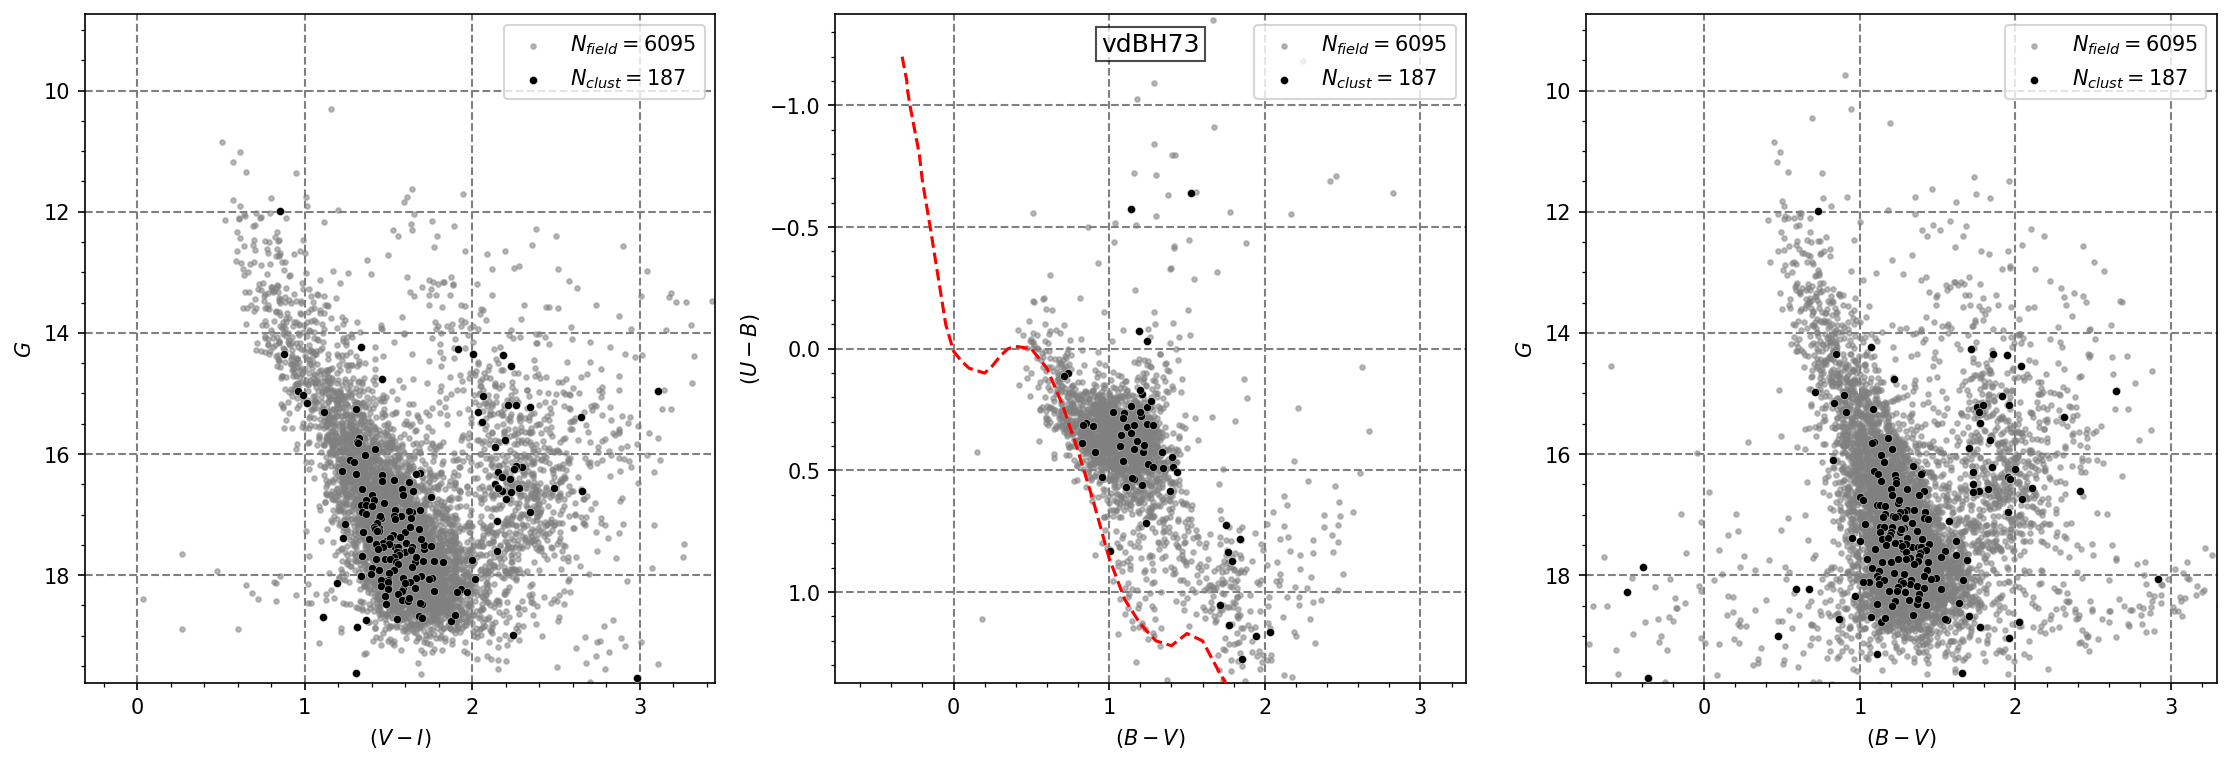
\includegraphics[width=\hsize]{figs/high_res/obs_vdBH73.png}
    \caption{From left to right: The $V$ vs $(B-V)$ , $V$ vs $(V-I)$ and
    $(B-V)$ vs $(U-B)$ diagrams for all the stars observed in the region of van
    den Bergh-Hagen 73.
    The red dashed line in the two color diagram gives the position of the ZAMS
    \citep{Aller1982}. Inserts in the upper right corner in each
    diagram contain the number of stars included in the respective figure.}
    \label{fig3}
\end{figure*}

\begin{figure*}[ht]
    \centering
    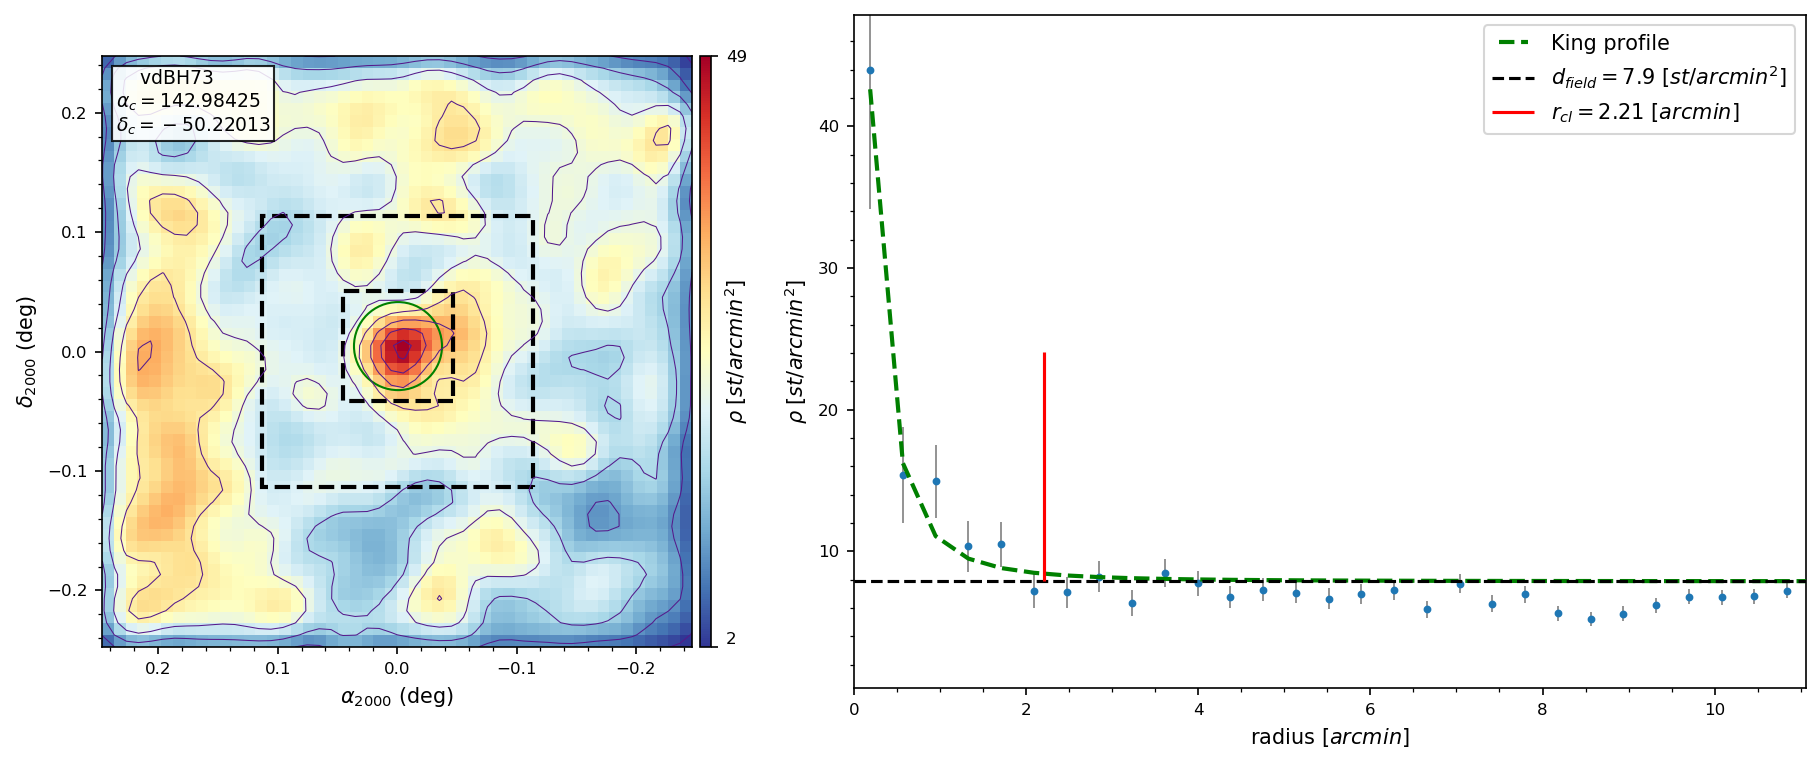
\includegraphics[width=\hsize]{figs/high_res/dmap_vdbh73.png}
    \caption{Left panel: The contour plot showing the position of the
    overdensity associated to vdBH 73. Green inner circle gives
    the cluster size while the two black dashed lines squares enclose the region
    used for \texttt{ASteCA} to estimate the field stars properties. Absolute
    coordinates in decimal format are indicated. The color scale at the right
    denotes the star number per square arcmin. Right panel: King profile is
    shown in dashed green line. The horizontal blue line is for the field
    mean star density. Vertical red line is set for the adopted cluster
    radius.The Poisson error ($\sqrt{N}$) of each curve point is shown with a
    vertical black line.}
    \label{fig4}
\end{figure*}

\begin{figure*}[ht]
    \centering
    \includegraphics[width=\hsize]{figs/high_res/cmds_vdbh73.png}
    \caption{From left to right: The $V$ vs $(B-V)$ , $V$ vs $(V-I)$ and
    $(B-V)$ vs $(U-B)$ clean diagrams after the removal by field interlopers
    made by \texttt{ASteCA} over vdBH 73.
    The color of each star reflects its membership
    probability. Corresponding values are in the color bar at the upper right
    corner in the $V$ vs $(B-V)$ diagram (left). Insert at the lower right
    corner in the $V$ vs $(B-V)$ diagram shows the number of stars used by 
    \texttt{ASteCA} to compare with synthetic clusters.
    Insert in the mid panel includes the final
    results for metallicity, $\log(age)$, $E_{(B-V)}$, the corrected distance
    modulus, and the cluster total mass provided by \texttt{ASteCA}. The green
    continuous line in the three diagrams is a reference isochrone. In
    particular, the green line in the color-color diagram, mid panel, shows the
    most probable $E_{(B-V)}$ value fitting found by \texttt{ASteCA}.}
    \label{fig5}
\end{figure*}

\begin{figure*}[ht]
    \centering
    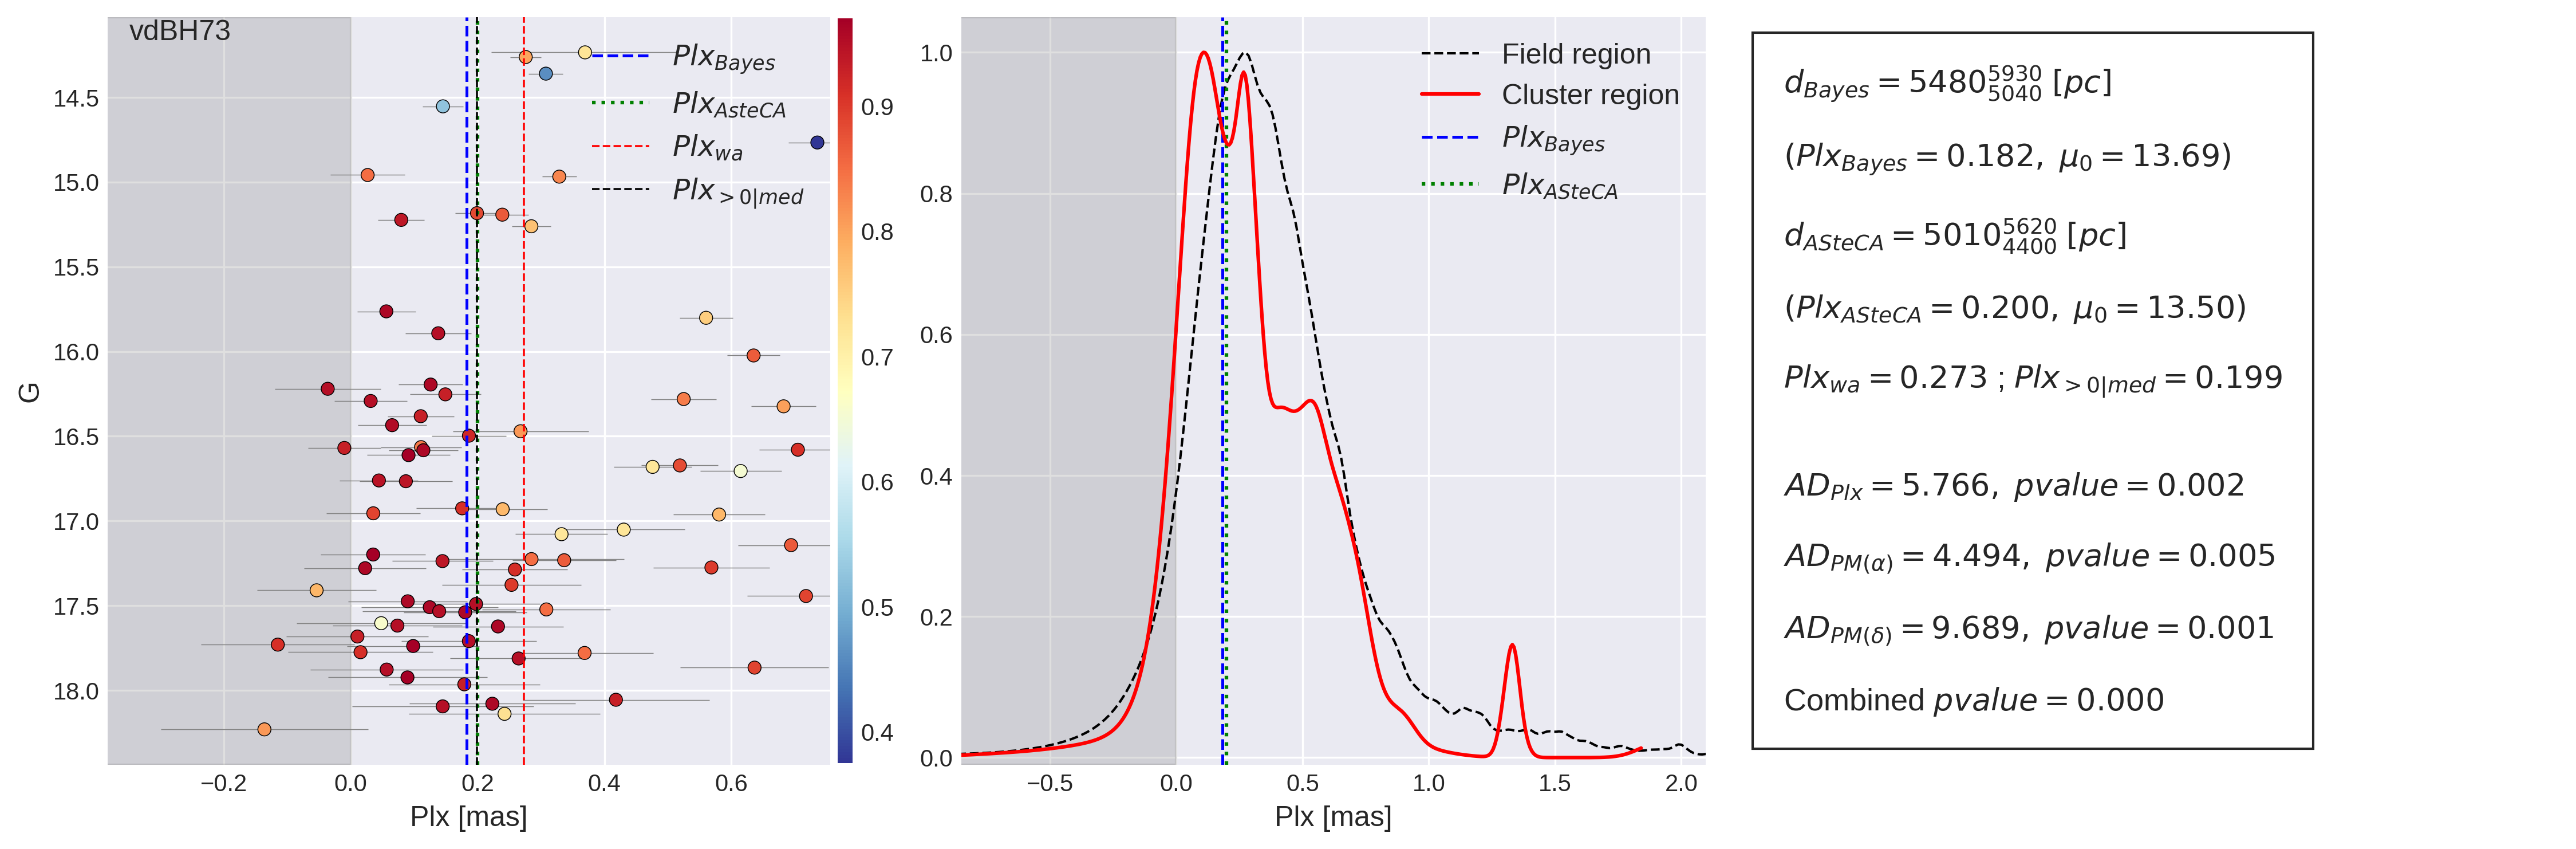
\includegraphics[width=\hsize]{figs/high_res/plx_vdBH73.png}
    \caption{Left panel: distribution of parallax for all stars with membership
    probabilities in the cleaned cluster region, as a function of the apparent
    magnitude $V$ (vertical color scale is for the star membership
    probability) in vdBH 73.
    Horizontal bars are the parallax errors as given by GAIA DR2. The different
    parallax value fittings are shown by dashed lines of different colors (see
    text). The mid panel is a normalized comparison between the parallax
    distributions inside the cluster region (red line) and outside it (dashed
    black line). The frame at the right summarizes the distances in parsecs
    according to the Bayesian analysis ($d_{Bayes}$) and \texttt{ASteCA} ($d_
    {ASteCA}$) followed by the parallax corresponding value, $Plx$, and
    corrected distance modulus ($\mu_0$). Both fittings are indicated by the
    vertical blue and green dashed lines. The last four text lines in the right
    panel are the AD values for $Plx$, $PM(\alpha)$, $PM(\delta)$ followed by
    the corresponding $p$-values and, finally the combined $p$-value.}
    \label{fig6}
\end{figure*}

The cluster vdBH 73 is placed in almost the center of the Vela
constellation well at the northeast border of the Carina Constellation. The
visual chart of the region in Fig. \ref{fig2} shows a small and compact grouping
of stars at the very center of the frame surrounded by a dense stellar field.
However, the inspection of the CCD and CMDs for all the observed stars in
Fig. \ref{fig3} gives no hints about the presence of a
cluster there. Basically, there are in the CMDs of Fig. \ref{fig3} few stars
above $V=15$ mag but at larger magnitudes the CMDs strongly widen surely due to
the presence of increasing visual absorption. In fact, the reddening in the
CCD, right panel in Fig. \ref{fig3}, is quite strong and displaces the bulk of
stars entirely toward the red side. Even some blue stars with negative $(U-B)$
values appear strongly affected by variable reddening.\\

The \texttt{ASteCA} spatial data processing shows a pronounced star overdensity
of 2.5 arcmin radius in the left panel in Fig. \ref{fig4} coincident with the
location expected for vdBH 73. This overdensity appears very well
detached from the field star mean density as seen in the RDP to the right.
Notice that the density peak is about five times above the mean for the field.\\

In the following step the removal of field interlopers by comparison with the
background field properties yielded the clean diagrams for all stars with
membership probability above 0.55 which are shown in Fig. \ref{fig5}. The clean
CMDs, left and right panels, put in evidence a cluster main sequence subtending
3 magnitudes and a giant branch with stars up to $V = 15.5$ mag. The clean CCD
in the middle panel shows the locus occupied by stars in vdBH 73,
completely unnoticed in the equivalent CCD of Fig. \ref{fig3}. All these stars
have membership probabilities between 0.55 and 0.91 favoring thus the true
nature of this object. This is: such a level of probability suggests that stars
in the adopted cluster region are --for the most part-- well detached, in terms
of their photometric characteristics and spatial distribution, from those
belonging to the cluster surroundings and therefore with low chance to be
confused with the stellar field. The best fitting of a synthetic cluster
yields the following facts:

\begin{itemize}
\item [a)] The cluster is immersed in a region of moderate absorption since the
mean of reddening comes to be $E_{(B-V)} = 0.74$, a value compatible with the
ones provided by \cite{Schlafly_2011} (hereafter S\&F2011) who
found a maximum $E_{(B-V)}$ of about 1.2 mag towards vdBH 73.
\item [b)] The free-absorption distance modulus turns out to be 12.32 placing
this object at 2.911 kpc from the Sun.
\end{itemize}

From the photometric point of view the existence of a well outlined cluster main
sequence and the high probability memberships of the stars seen in it confirm
the real entity of vdBH 73. However, the usage of parallax data
from GAIA, see Fig. \ref{fig6}, shows a huge difference in distance reaching
up 1.5 kpc in the sense that GAIA DR2 parallaxes place the cluster farther than
photometry does. The Anderson-Darling test applied to parallax and proper motion
data demonstrates that the null hypothesis for the $PM(\alpha)$ distribution
cannot be definitely rejected since the AD value is smaller than 1.961,
associated with the 5\% critical value. It can nonetheless be rejected in the
cases of $Plx$ and $PM(\delta)$, and the combined $p$-value is small enough to
reject the null hypothesis.\\

We conclude from our analysis that van den Bergh 73 is an old cluster around
$2511\times10^6$ years old.



% ---------------------------------------------------------------------
\subsection{NGC 4349}

\begin{figure*}[ht]
    \centering
    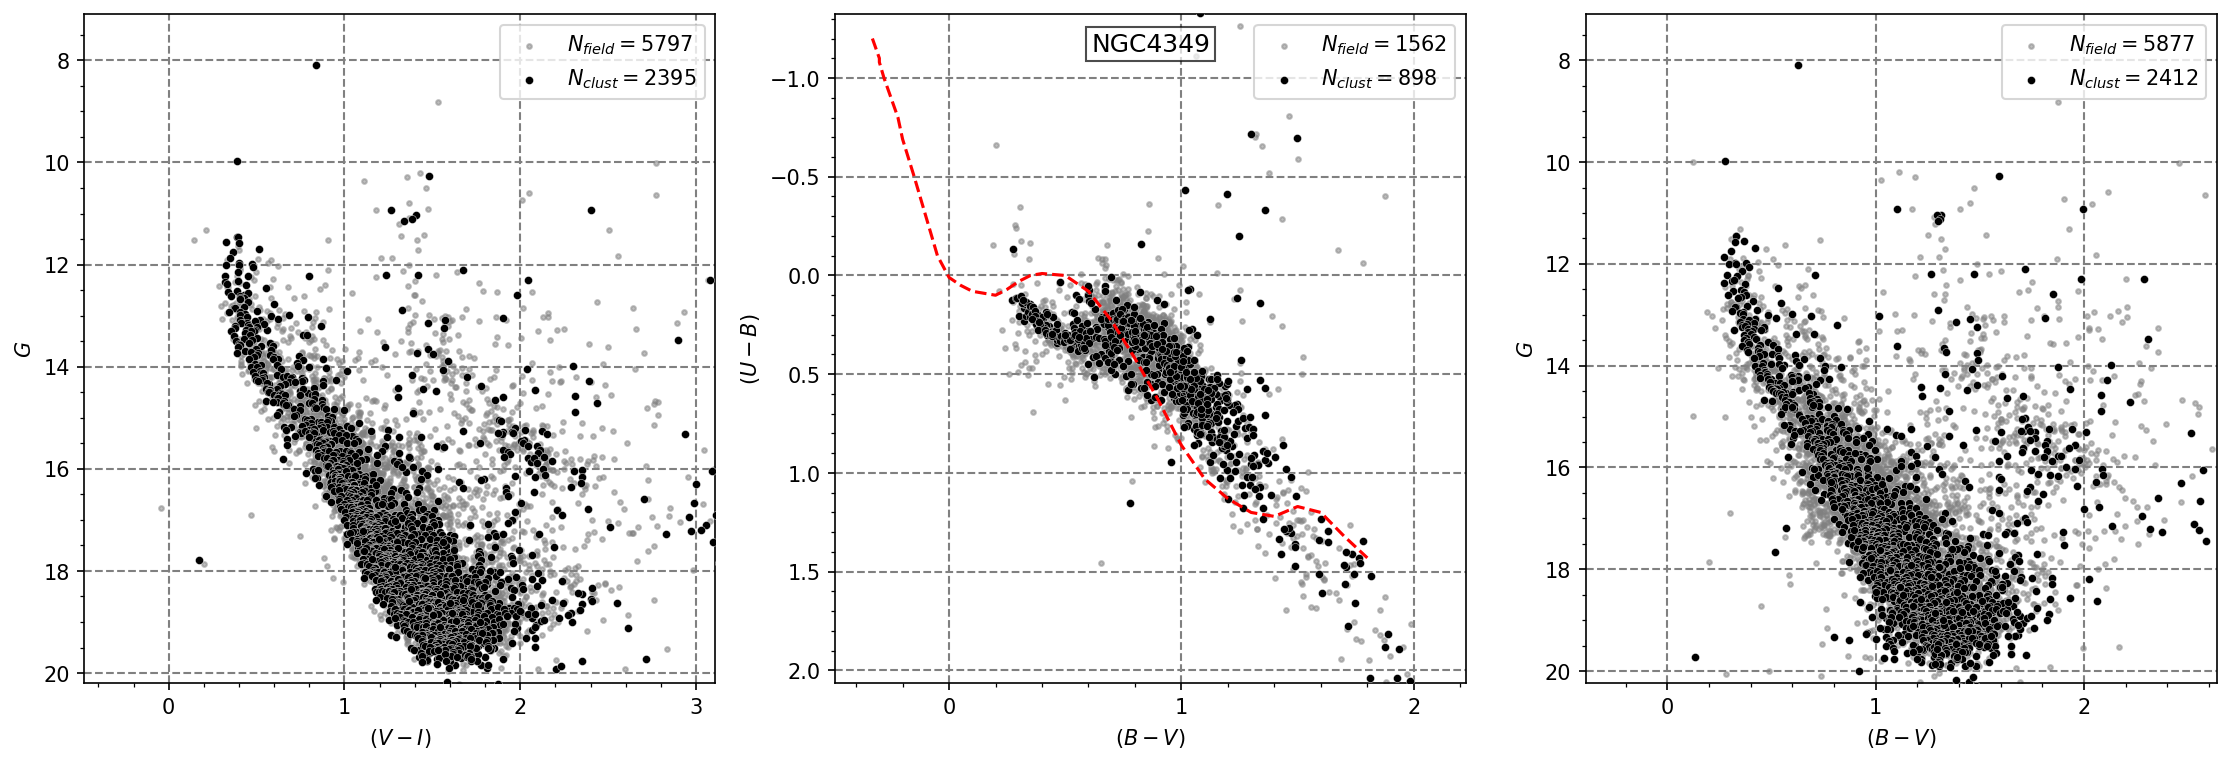
\includegraphics[width=\hsize]{figs/high_res/obs_NGC4349.png}
    \caption{Idem Fig. \ref{fig3} for NGC 4349.}
    \label{fig63}
\end{figure*}
\begin{figure*}[ht]
    \centering
    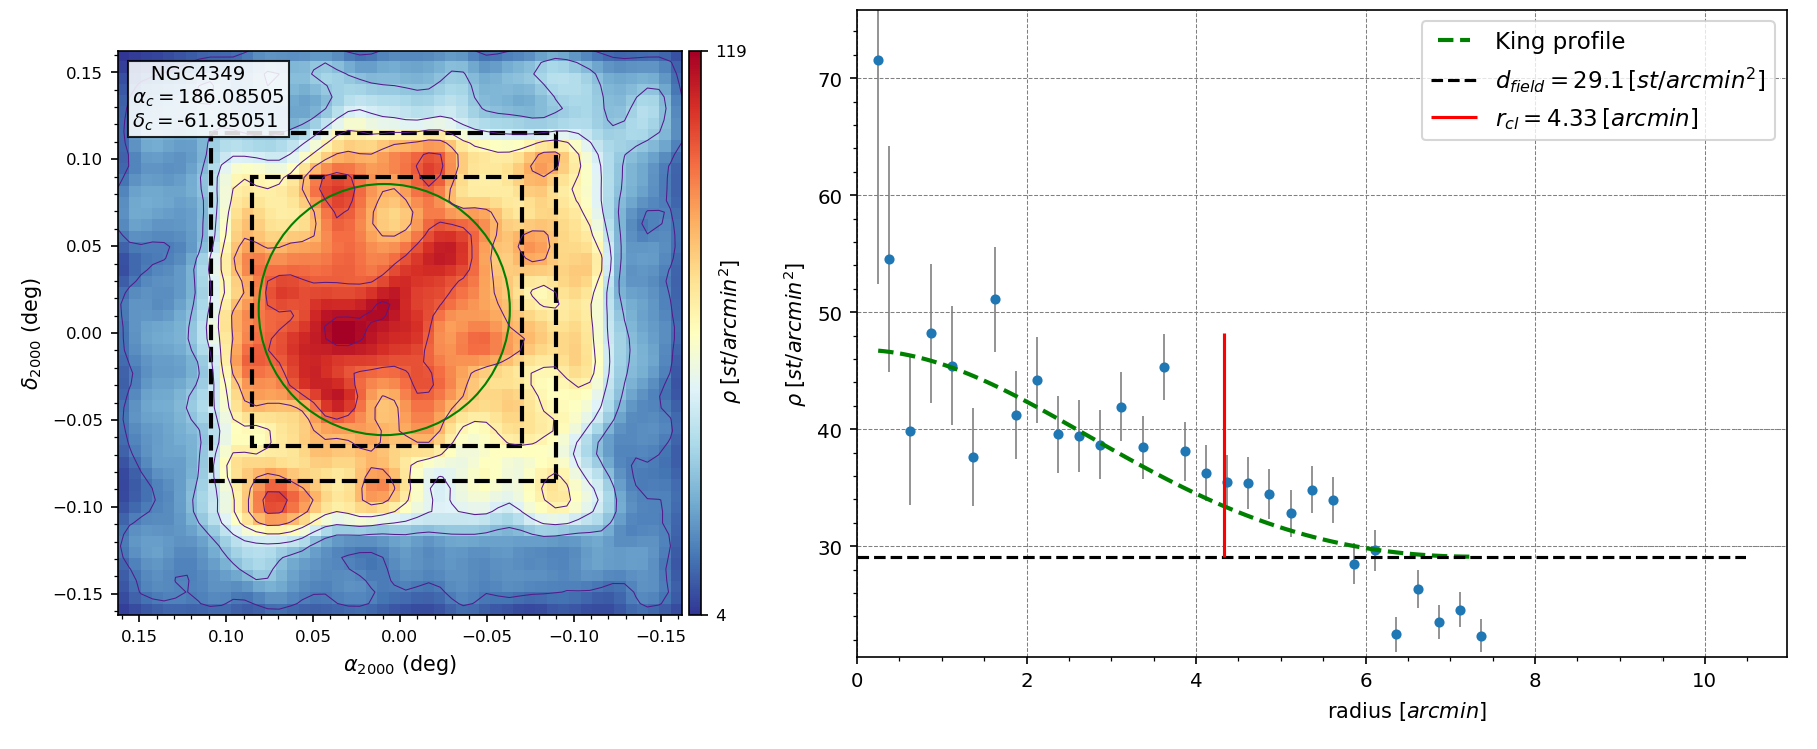
\includegraphics[width=\hsize]{figs/high_res/dmap_ngc4349.png}
    \caption{Idem Fig. \ref{fig4} for NGC 4349.}
    \label{fig64}
\end{figure*}
\begin{figure*}[ht]
    \centering
    \includegraphics[width=\hsize]{figs/high_res/cmds_ngc4349.png}
    \caption{Idem Fig. \ref{fig5} for NGC 4349.}
    \label{fig65}
\end{figure*}
\begin{figure*}[ht]
    \centering
    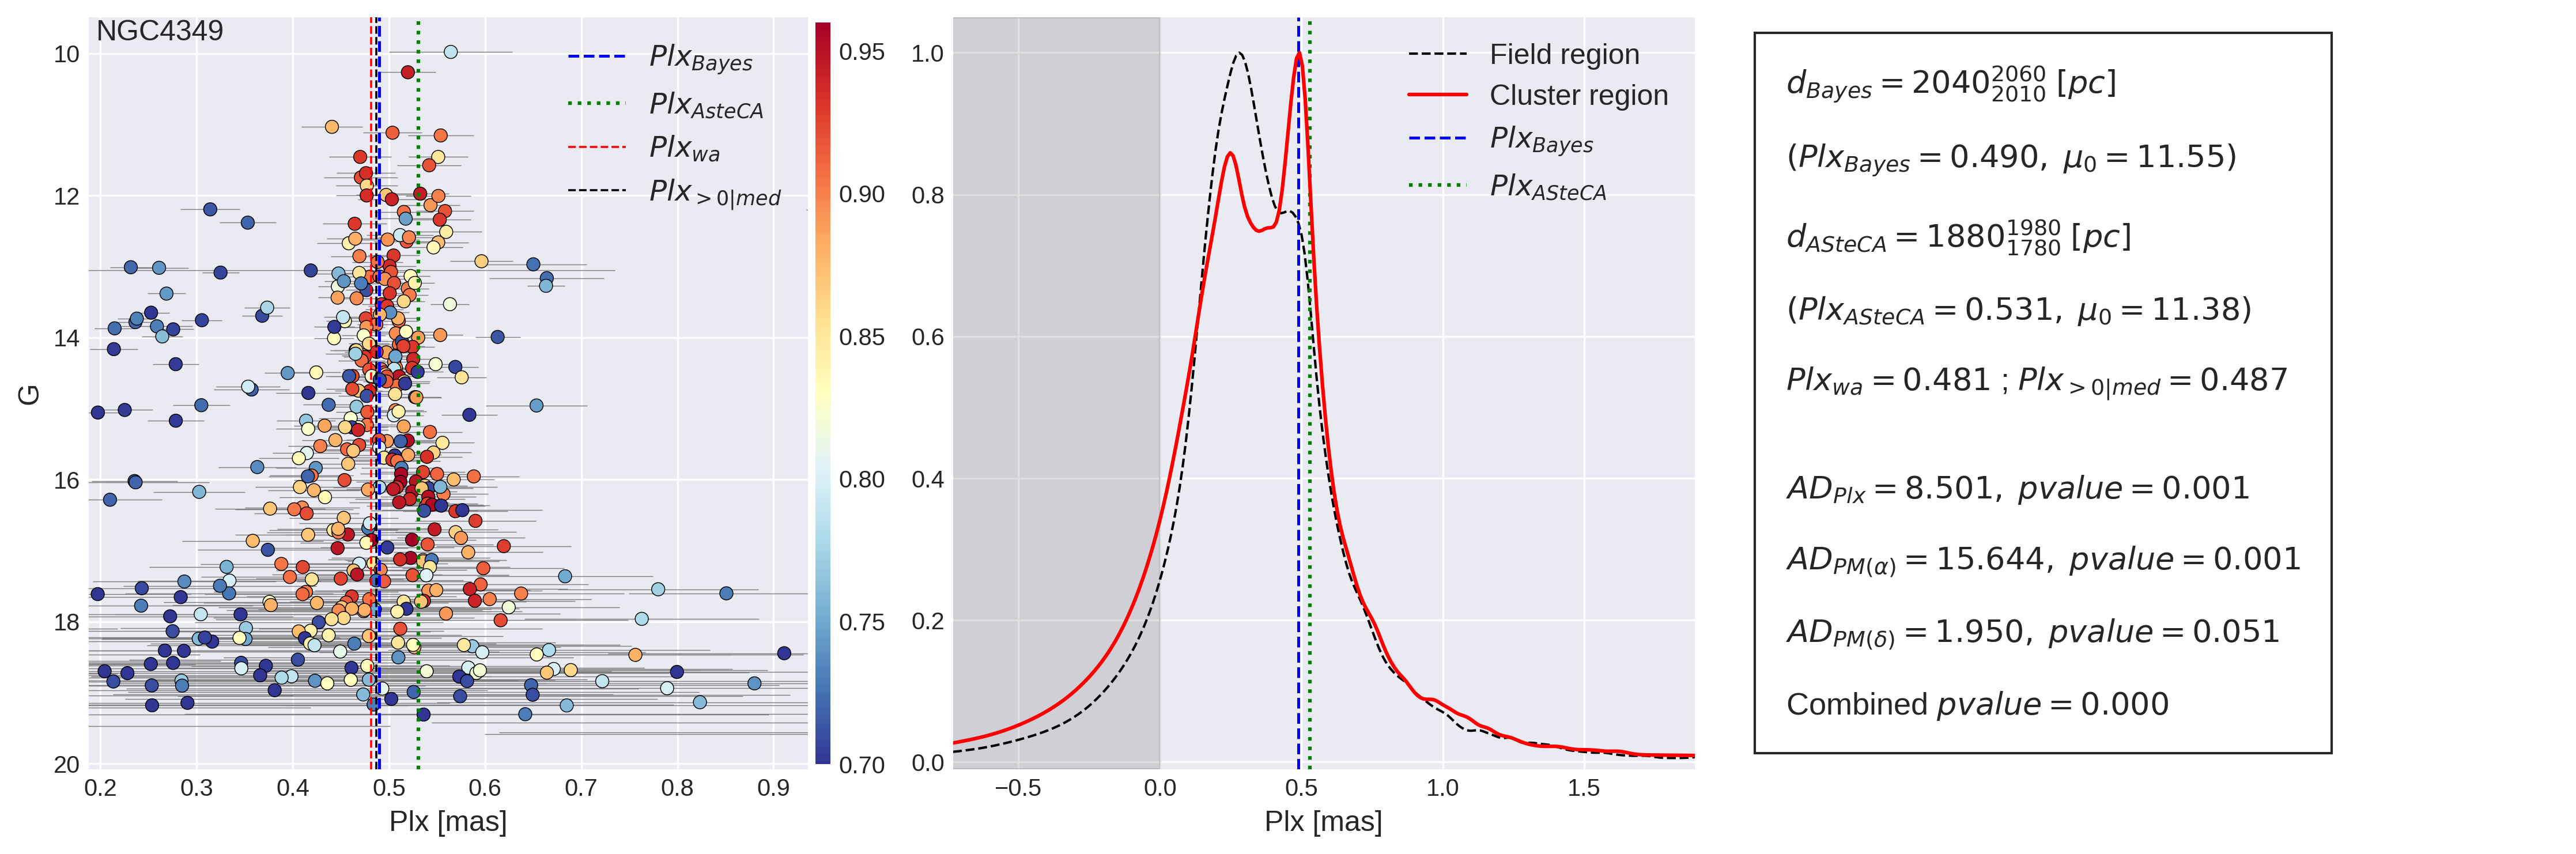
\includegraphics[width=\hsize]{figs/high_res/plx_NGC4349.png}
    \caption{Idem Fig. \ref{fig6} for NGC 4349.}
    \label{fig66}
\end{figure*}


This is a Crux constellation object, placed slightly south of the Crux geometric
center. At first glance, the $V$ image in Fig. \ref{fig2} shows a
distinguishable star accumulation. The overall photometric CCD and CMDs in
Fig.~\ref{fig63} show a prominent star sequence emerging at $V=16$ mag from the
usual stellar structure produced by disc stars. The CCD makes more evident the
presence of a reddened but compact sequence of blue stars placed immediately
below the first knee of the intrinsic line. Apart from this, other bluer stars
appear for $(U-B)$ values smaller than 0.0.\\ 

\texttt{ASteCA} analysis revealed an extended overdensity of up to 20 stars per
square arcmin reflected by a prominent but a tiny RDP with a radius of 4.5
arcmin depicted in the panels of Fig. \ref{fig64}.
The \texttt{ASteCA} estimation of memberships shows that inside the adopted
cluster radius the probability values go from 0.63 to 0.96 in the respective CCD
and CMDs of Fig. \ref{fig65}. So, it is clear that probable members of the
cluster detach easily from the field region stars photometric properties. If
attention is drawn to the largest probabilities (say above 0.7, starting in
light yellow symbols) there appears in the three diagrams a narrow cluster.
Comparison with synthetic clusters yielded
that NGC 4349 is a cluster with the following properties:

\begin{itemize}
    \item [a)] A color excess of $E_{(B-V)}= 0.40$ is found for the best fitting
    synthetic cluster. Since the maximum color excess provided by
    S\&F2011 in this location is 2.83 one concludes that most of the
    absorption is produced behind the position of NGC 4349.
    \item [b)] The absorption free distance modulus of NGC 4349 is 12.1,
    placing it at a distance of $d=2.630$ kpc from the Sun. 
\end{itemize}

NGC 4349 is the only cluster in our sample with previous photographic photometry
in the $UBV$ system performed by \cite{Lohmann_1961}. Given the usual large
differences between photographic and CCD photometry we performed no comparison
between the Lohmann data-set and ours. According to \cite{Lohmann_1961}, NGC
4349 is located at a distance of $d=1.7$ kpc, far enough from our estimate.
However, coincidences in terms of reddening, size and background star density
have been found since Lohmann stated a cluster reddening of $E_{(B-V)}=0.38$
and similar cluster size. On the other hand, the Kharchenko
Atlas\footnote{\url{https://webda.physics.muni.cz/cocd.html}}
\citep{Kharchenko_2005} gives a reddening value of $E_{(B-V)} = 0.38$ quite
similar to ours although the distance reported, $d=2.1$ kpc, is slightly below
our estimate.
It is worth noting that the distance found for this cluster using GAIA DR2
parallax data, processed with the Bayesian method described in Sect.~
\ref{ssec:gaia_data}, is remarkably close to the photometric distance found by 
\texttt{ASteCA}: 2620 pc vs 2630 pc, respectively.

Parallax and proper motion distributions were tested using the Anderson-Darling
statistics. With the exception of the comparison in the case of $PM(\delta)$
(where both samples, cluster and field, seem to come from the same distribution
at a critical value of 8\%) the remaining two tests report quite different
samples confirming, together with the photometric results, the true nature of
NGC 4349.\\

High probability values for stars inside the overdensity confirm the
true nature of this object since the over density and the density profile
are followed by a very well defined and extended photometric counterpart.
Since all these facts are self-consistent, we are confident that NGC 4349 is
an open cluster around $355\times10^6$ years old.
The Kharchenko Atlas gives quite a similar value for the cluster age, reporting
$\log(t)=8.32$ equivalent to $209\times10^6$ yrs.



% ---------------------------------------------------------------------
\subsection{Ruprecht 87}

\begin{figure*}[ht]
    \centering
    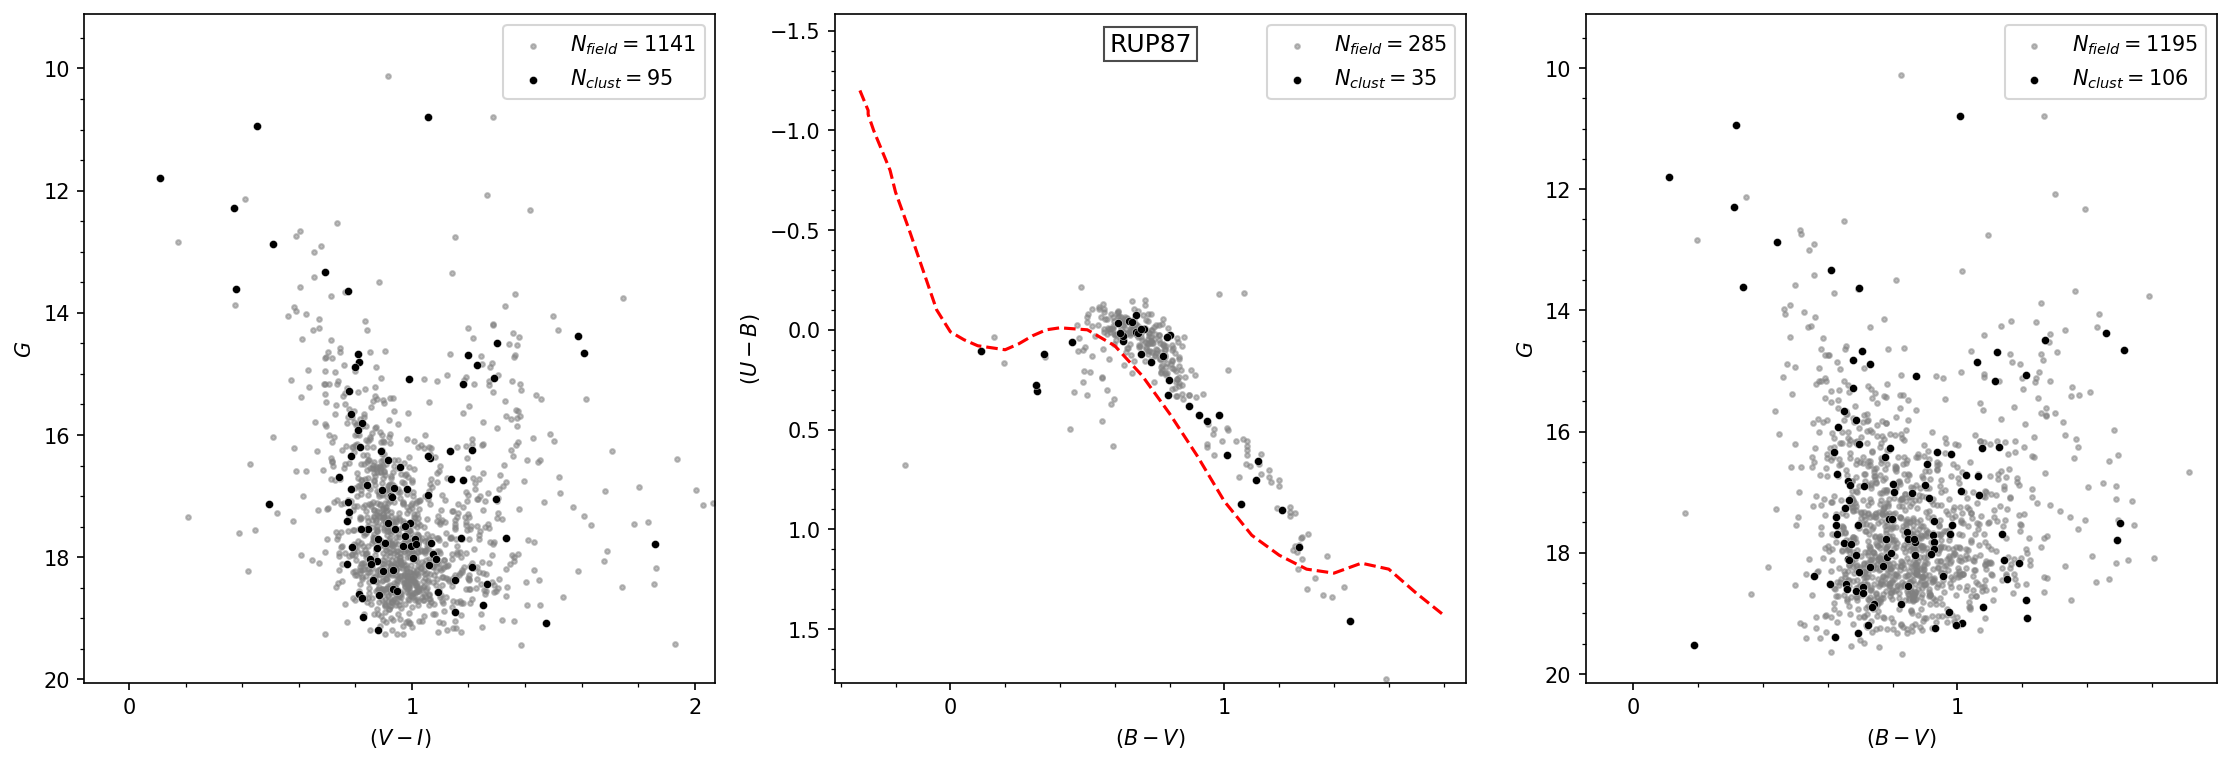
\includegraphics[width=\hsize]{figs/high_res/obs_RUP87.png}
    \caption{Idem Fig. \ref{fig3} for RUP 87.}
    \label{fig23}
\end{figure*}
\begin{figure*}[ht]
    \centering
    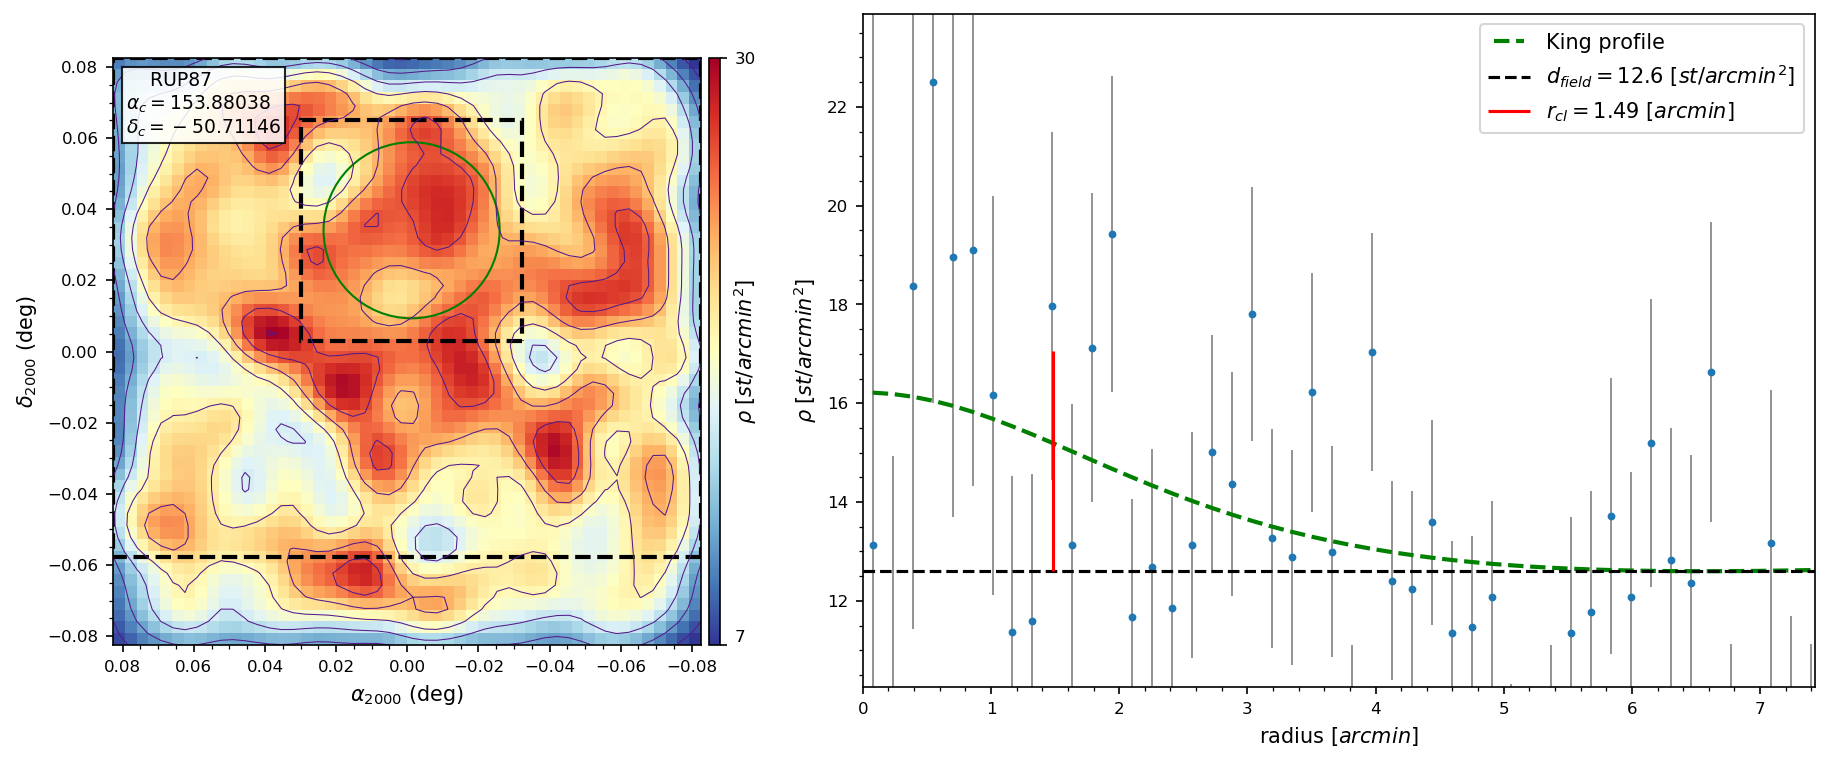
\includegraphics[width=\hsize]{figs/high_res/dmap_rup87.png}
    \caption{Idem Fig. \ref{fig4} for RUP 87.}
    \label{fig24}
\end{figure*}
\begin{figure*}[ht]
    \centering
    \includegraphics[width=\hsize]{figs/high_res/cmds_rup87.png}
    \caption{Idem Fig. \ref{fig5} for RUP 87.}
    \label{fig25}
\end{figure*}
\begin{figure*}[ht]
    \centering
    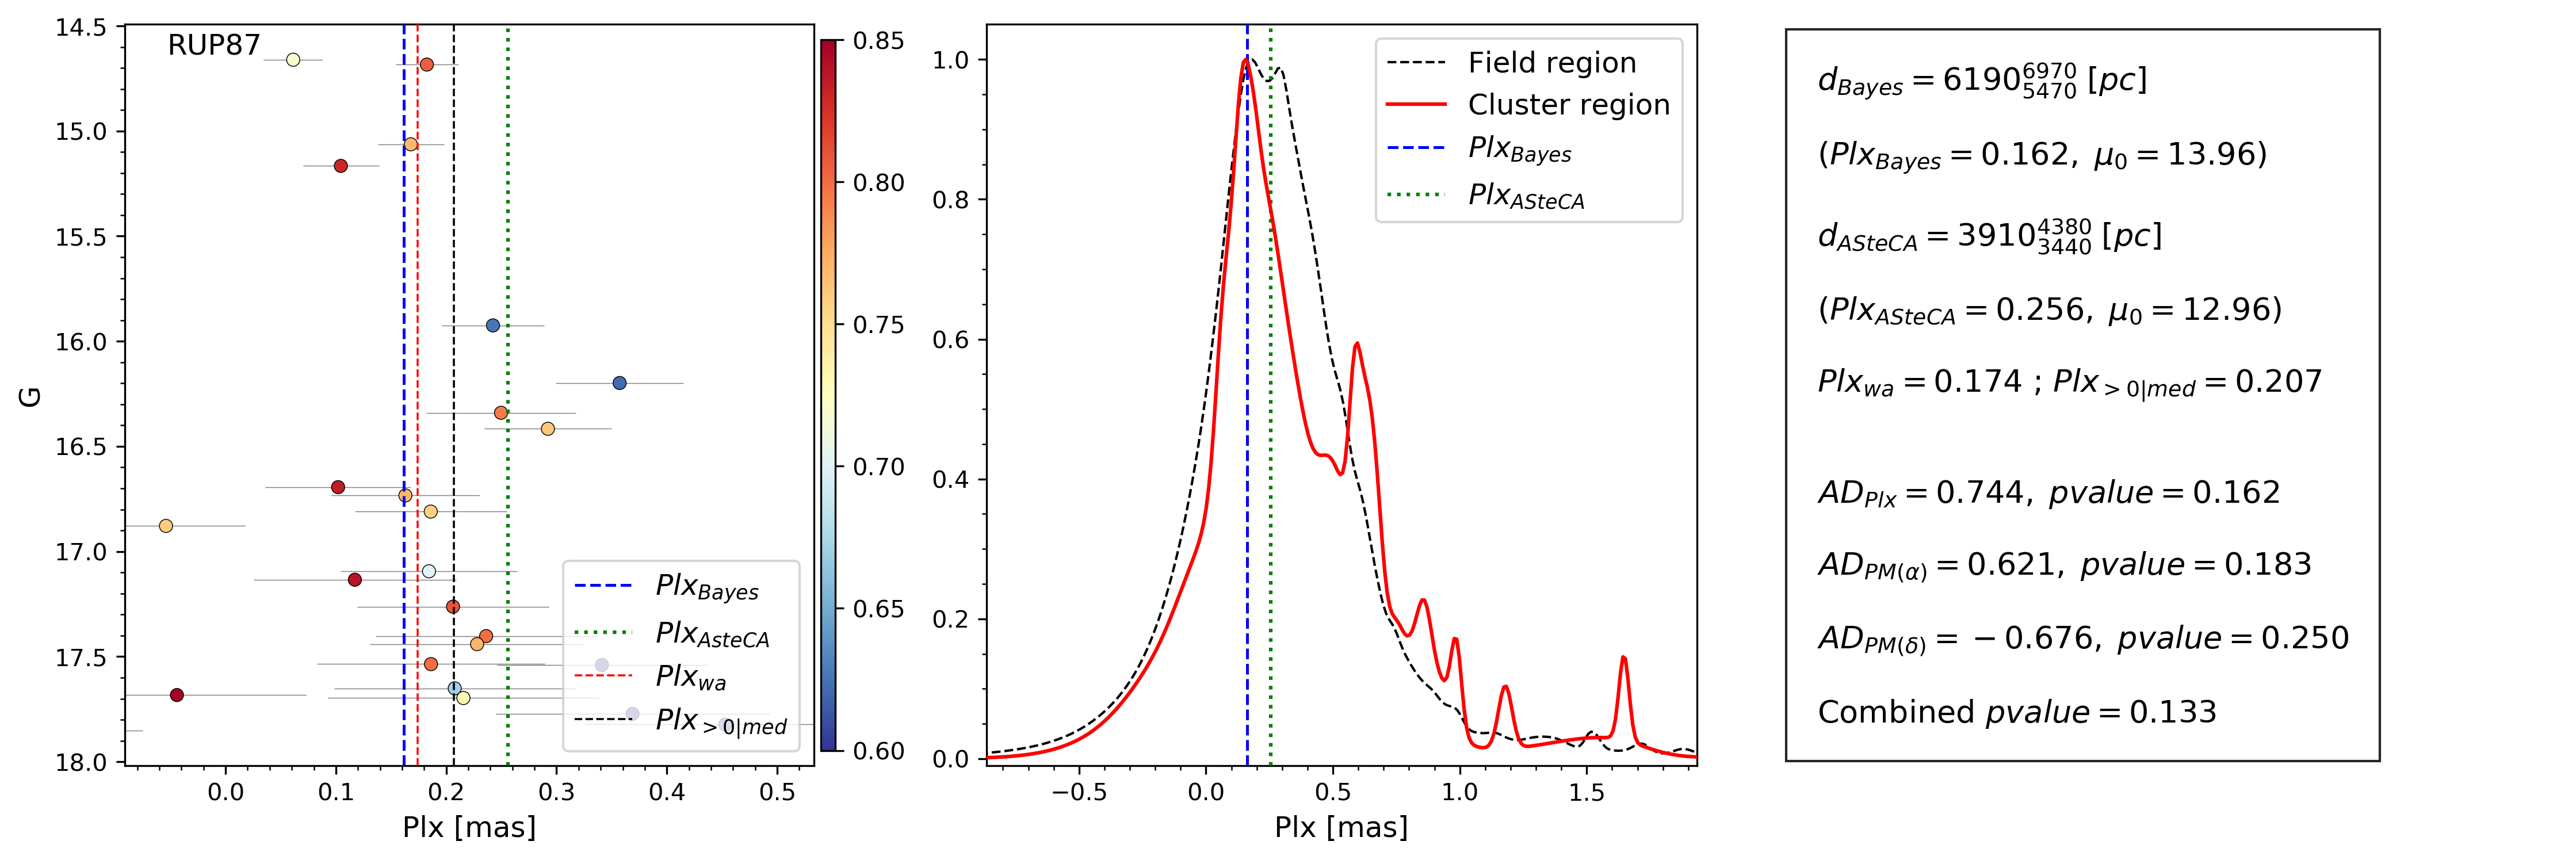
\includegraphics[width=\hsize]{figs/high_res/plx_RUP87.png}
    \caption{Idem Fig. \ref{fig6} for RUP 87.}
    \label{fig26}
\end{figure*}

RUP 87 is in the east side of the Vela constellation. According to the
respective Fig. \ref{fig2} there is no relevant feature but a rather poor and
boring stellar field. The first glance impression is confirmed in the
photometric diagrams since no appreciable stellar structure
defining the presence of an open cluster is present in the overall CMDs of Fig.
\ref{fig23}. The few stars with $(U-B)$ measures plotted in the respective
color-color magnitude resemble a typical CCD of a galactic field dominated by a
handful of late $F$ and $G$-type stars followed by a pronounced tail of red
stars presumably of evolved types. Perhaps stars in the region $0<(U-B)<0.5$
and $0<(B-V)<0.6$ are reddened early $A$ or/and late $B$-types.\\

Accordingly, after many essays \texttt{ASteCA} could not define the presence of
an overdensity as obviously seen in Fig. \ref{fig24}. The inability of our code
to identify any overdensity simply means that the potential locus occupied by
the cluster RUP 87 is not unambiguously separated from the field background
stars. So, after many attempts to state the place of the cluster we decide to
focus the attention in the region encircled by a green line. However, the RDP
emerging from this analysis is not only quite noisy but it is hard to establish
the mean value of the background density. Notice that only 30 stars remain in
the region adopted. The estimation of the memberships and the not so clear clean
CCD and CMDs in Fig. \ref{fig25} reflects the difficulty since stars inside the
adopted cluster area have membership values ranging from 0.12 to 0.54 so that
they may also belong to the surrounding field.\\

As seen in Fig. \ref{fig26} the Anderson-Darling test values for $Plx$ and
proper motions do not confirm clear differences between the cluster region and
the stellar background in terms of kinematics and distance. The poverty of the
photometric diagrams and the analysis of GAIA data are all against the true
existence of a cluster in the region RUP 87. In our interpretation this is
not a real entity but a fluctuation of the star field.





%================================================================
\section{Discussion of results and concluding remarks}
\label{sec:results_concl}

In the precedent section we have determined the true nature of sixteen potential
open clusters located in a Galaxy sector covering from $290^\circ$ to
$320^\circ$ approximately in galactic longitude, and the formal
galactic plane at $b = 0^\circ$.
The cluster parameter estimations presented in this article
are based in precise $UBVI$ photometry carried out in a semi-automatic way by
our code \texttt{ASteCA}. The code looks for a meaningful stellar overdensity
assigning membership probabilities by comparison with the surrounding stellar
field.
The next step establishes the physical properties of the best synthetic cluster
that fits the distribution of cluster members in the CMDs and the CCD.
Through this process reddening, distance, age, mass, and metallicity are
given.
The most relevant inconvenient we have found with the present cluster
sample resides in the fact that they are extremely faint, which becomes evident
by visual inspection in the overall CCD and CMD.
To make things worse the $(U-B)$ index has been majorly available for
the bright and blue stars which reduced considerably the data analysis space.
Despite this we were able to keep the reddening solutions under control and
obtain reliable distances estimations.

We can discard the following objects from our cluster sample: RUP 87,
vdBH91, RUP 88, Lynga 15, Loden 565 and NGC 4230 since they are most probably
random stellar fluctuations. The results for true and probable open clusters are
shown in Table \ref{tab:final_tab} in self-explicative format.\\

\begin{table*}[ht]
\centering
\begin{tabular}{lcccccc}
\hline
 \emph{Cluster name} & z & $E_{(B-V)}$ & \emph{Age} & \emph{Mass} &
 $d_{ASteCA}$ & $d_{Bayes}$
 \\
& & & $(10^6 yr)$ & $(M_{\odot})$ & $(kpc)$ & $(kpc)$\\
 \hline\hline
 vdBH 73 & 0.0185$\pm0.0047$ & 0.74$\pm0.01$ & 2511$\pm1400$ & 2250$\pm150$ &
 2.911$\pm0.27$ & 4.372$\pm0.4$\\
 RUP 85 & 0.0145$\pm0.0018$ & 0.77$\pm0.02$ & 891$\pm100$ & 3350$\pm550$ &
 3.420$\pm0.13$ & 4.537$\pm0.23$ \\
  vdBH 85 & 0.0145$\pm0.0026$ & 0.34$\pm0.03$ & 5011$\pm580$ & 4800$\pm160$ &
  4.246$\pm0.2$ & 5.145$\pm0.34$ \\
 vdBH 87 & 0.0205$\pm0.005$ & 0.56$\pm0.03$ & 630$\pm370$ & 1800$\pm220$ &
 1.906$\pm0.1$ & 2.192$\pm0.08$ \\
 TR 12* & 0.0115$\pm0.003$ & 0.26$\pm0.01$ & 446$\pm200$ & 700$\pm200$ &
 3.048$\pm0.18$ & 3.717$\pm0.15$ \\
 vdBH 92 & 0.0145$\pm0.003$ & 0.58$\pm0.01$ & 112$\pm100$ & 500$\pm100$ &
 1.941$\pm0.08$ & 2.369$\pm0.11$ \\
 TR 13 & 0.0205$\pm0.0034$ & 0.50$\pm0.01$ & 56$\pm10$ & 2050$\pm170$ &
 4.467$\pm0.16$ & 4.424$\pm0.16$ \\
 vdBH 106 & 0.0145$\pm0.0034$ & 0.33$\pm0.05$ & 1122$\pm220$ & 1300$\pm360$ &
 4.406$\pm0.52$ & 3.757$\pm0.44$ \\
 RUP 162* & 0.0075$\pm0.0029$ & 0.25$\pm0.01$ & 14$\pm14$ & 1650$\pm280$ &
 2.399$\pm0.02$ & 3.464$\pm0.18$ \\
 NGC 4349 & 0.0155$\pm0.0028$ & 0.40$\pm0.01$ & 354$\pm40$ & 4350$\pm120$ &
 2.630$\pm0.02$ & 2.620$\pm0.16$ \\
 \hline
\end{tabular}
\caption{The symbol ``*'' indicates probable clusters. The $d_{Bayes}$ values
are those obtained using the Bayesian method and the Lindegren et al. bias
correction on the parallax data. Uncertainties for the fundamental parameters are
shown in parenthesis.}
\label{tab:final_tab}
\end{table*}

In an ulterior step we draw the attention to GAIA DR2 parallax data to perform a
fast computation of distances and compare them with the findings from the
analysis of the photometry. In this context $Plx$ data were cross correlated
with our photometry and processed within a Bayesian framework.
% while $PM(\alpha)$ and $PM(\delta)$
% data were used as an additional control regarding different kinematic properties
% for cluster areas and the stellar backgrounds.\\
As seen in the last two columns of Table \ref{tab:final_tab} distances from
\texttt{ASteCA} are almost always a bit smaller than the ones coming
from our computation of parallax values provided by GAIA DR2, and corrected
according to the Lindegren et al. bias (0.029 mas). The exceptions are
TR 13, NGC 4349, and vdBH 106 which show smaller
photometric distances (particularly vdBH 106).
%
The situation is more clearly shown in Fig. \ref{fig67} (left) with a plot of 
\texttt{ASteCA} distances against those obtained from GAIA DR2 parallaxes,
shifted by the Lindegren et al. bias.
%
Two clusters, NGC 4349 and TR 13, along the identity line show very good
agreement between both distances. Differences reaching over 1 kpc (huge amount
indeed) are found for RUP 162, vdBH 73 and RUP 85.

If we instead add 0.075 mas to the parallax data following the results
recently presented in \cite{Xu_2019}, we see that the agreement between
photometric and GAIA DR2 distances improves substantially as shown in Fig. 
\ref{fig67} (right).
%
The general mean differences between photometric distances (estimated with 
\texttt{ASteCA}) and parallax distances (GAIA DR2 parallax data corrected by a
bias value and processed with a Bayesian method) are of $\sim-522$ pc and only
$\sim6$ pc, using the bias corrections from Lindegren et al. and Xu et al.
respectively. This tends to confirm that a larger bias correction for the
parallax is needed than that proposed by Lindegren et al.

Three clusters show no good agreement between photometric and parallax distances
with either bias correction: RUP 162, vdBH 73, and van den
Bergh-Hagen 106. vdBH 73 is well defined but faint while
vdBH 106 shows a very dispersed sequence in its CMD.
In the case of RUP 162 we have shown in Appendix~\ref{app:rup162} that this
cluster is not well structured despite some stars in the cluster region showing
large probability values.

% If we add 0.1 mas following the warning from \cite{Lindegren_2018} we see that
% the agreement between photometric and GAIA distances is excellent. The arrows in
% Fig. \ref{fig67} point out the positions occupied by these objects indicated
% with red filled circles. We add this quantity not only to these three clusters
% but also to TR 12 and vdBH 92 achieving a good agreement
% too. vdBH 73 and vdBH 85 are well defined but
% faint and in the case of RUP 162 we have shown in
% Appendix~\ref{app:rup162} that this cluster is not well structured despite some
% stars in the cluster region showing large probability values. Something similar
% happens with vdBH 92, while in the case of TR 12 the
% cluster is again not well defined from a photometric point of view but the
% Anderson-Darling tests suggest strong variations between proper motions and
% parallaxes confirming the real entity of this object. The other two separated
% objects vdBH 106 and vdBH 85 have no satisfying
% solution neither adding nor removing 0.1 mas since the situation gets worse.\\

\begin{figure*}[ht]
    \centering
    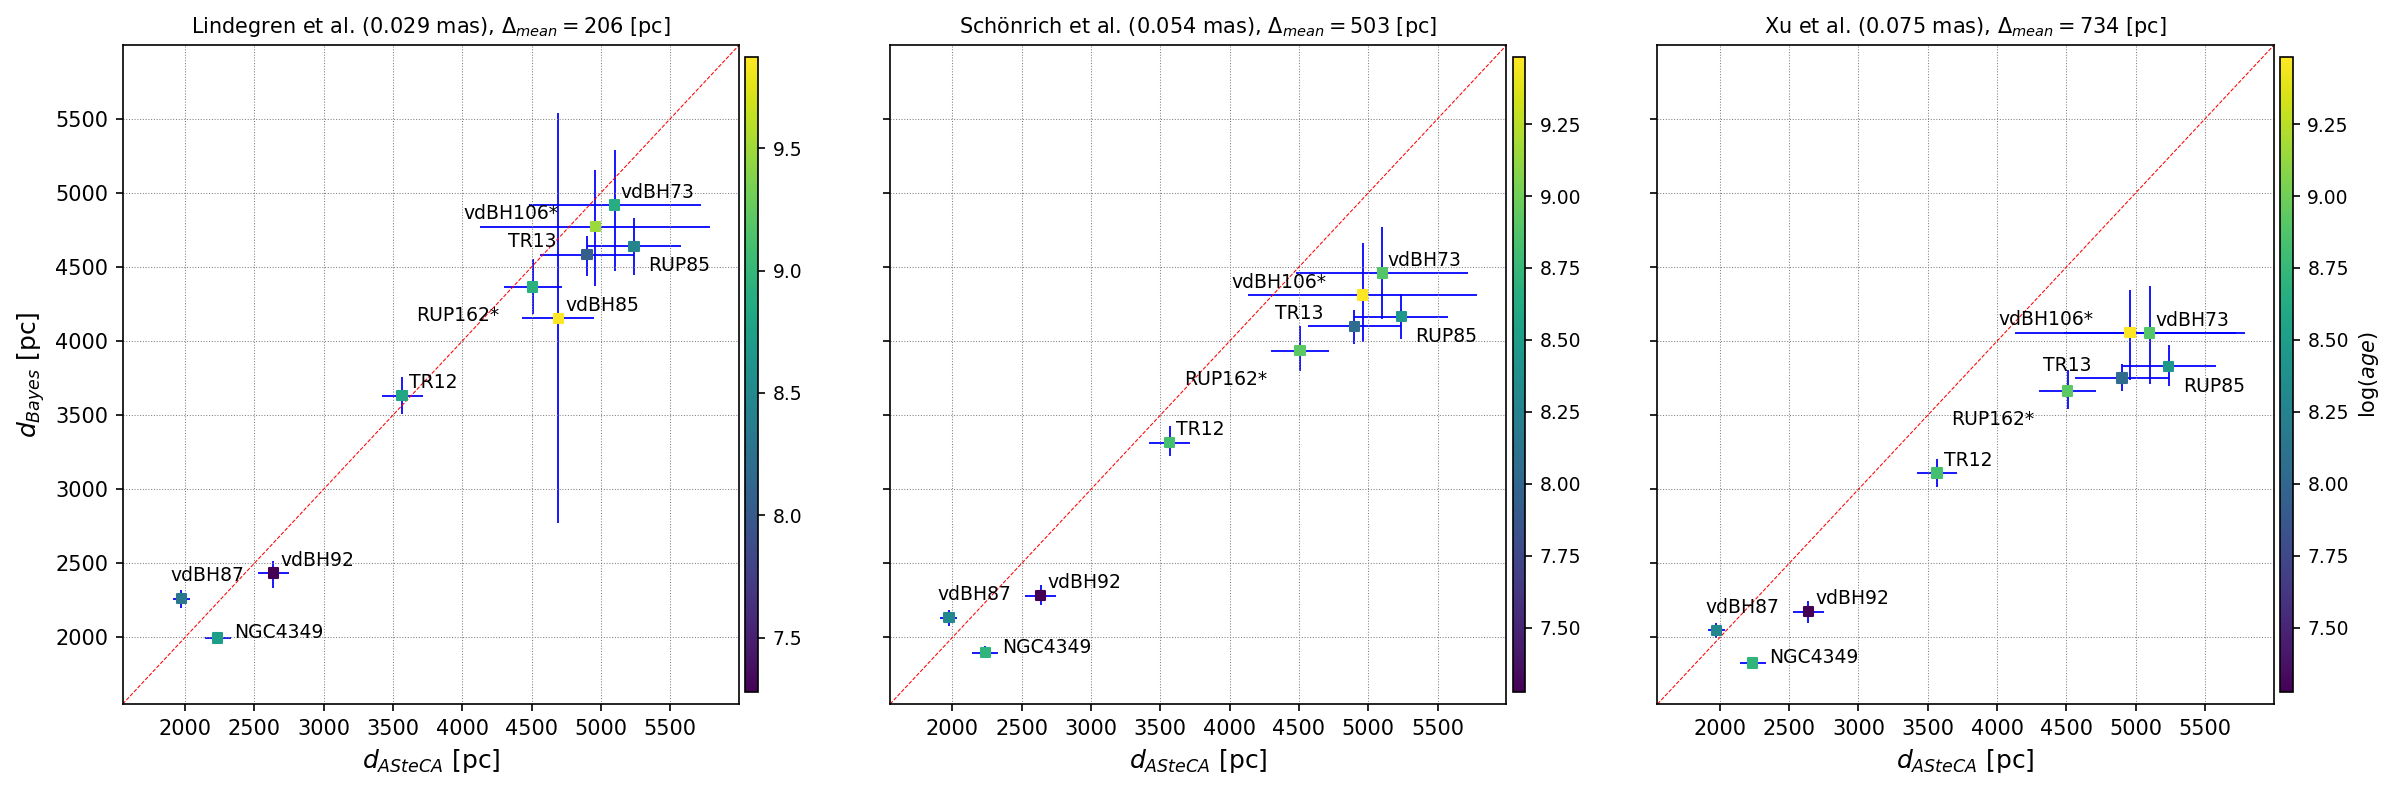
\includegraphics[width=\hsize]{figs/high_res/dist_comparision1.png}
    \caption{\texttt{ASteCA} (photometric) vs Bayesian (parallax) distances for
    the present sample, with bias corrections from Lindegren et al. (left), and
    Xu et al. (right). Error bars are indicated along with the cluster
    names. Red dashed-dotted line is the $x = y$ identity expression. The mean
    of differences between ASteCA and others distances is shown on top of the
    figures.}
    \label{fig67}
\end{figure*}

We conclude that by adding 0.029 mas to the cluster computed parallaxes from
GAIA DR2 parallax data the level of agreement with the photometric distances is
reasonable for near clusters, and is really good for robust objects like
TR 13 and NGC 4349.
For other objects the gap between photometric and parallax distances narrows
when 0.075 $\mu$as is applied instead, but the decision of adding
either quantity becomes somewhat arbitrary.
In Fig.~\ref{fig:dist_compar2} we compare the photometric distances
estimated by \texttt{ASteCA} with the distances estimated using GAIA DR2 data
with no bias corrections. The overall offset
appears to be $\sim0.09$ mas, much closer to the Xu et al. bias than the
Lindegren et al. bias.\\

\begin{figure}[ht]
    \centering
    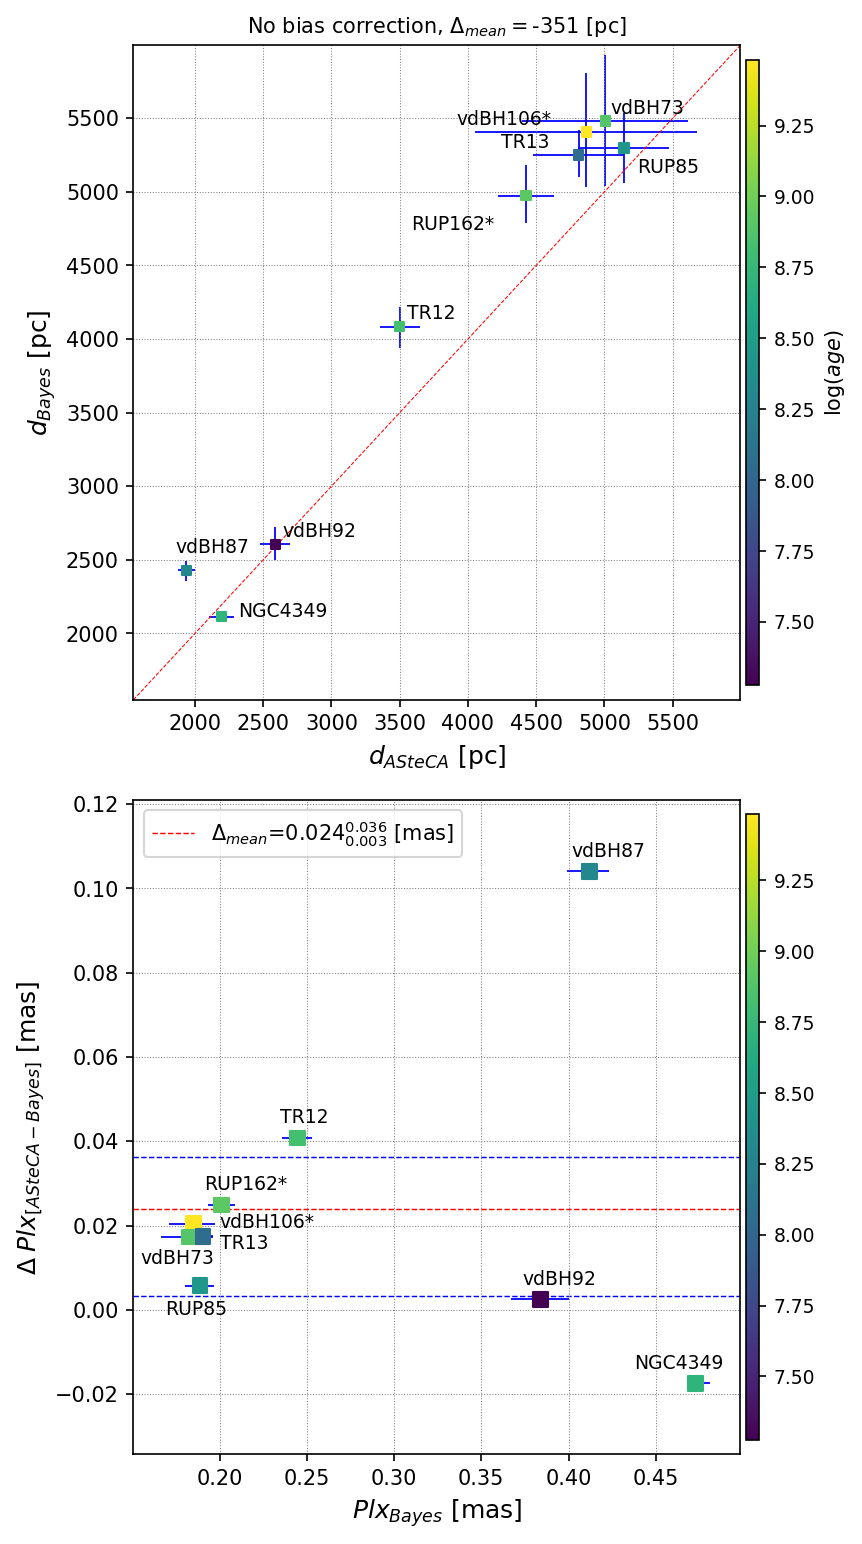
\includegraphics[width=\hsize]{figs/high_res/dist_comparision2.png}
    \caption{Offset between \texttt{ASteCA} photometric distances (expressed
    as parallax) and Bayesian parallaxes estimated using GAIA DR2 data with no
    bias correction, for the 10 clusters listed in Table~\ref{tab:final_tab}.}
    \label{fig:dist_compar2}
\end{figure}

\begin{figure}[ht]
    \centering
    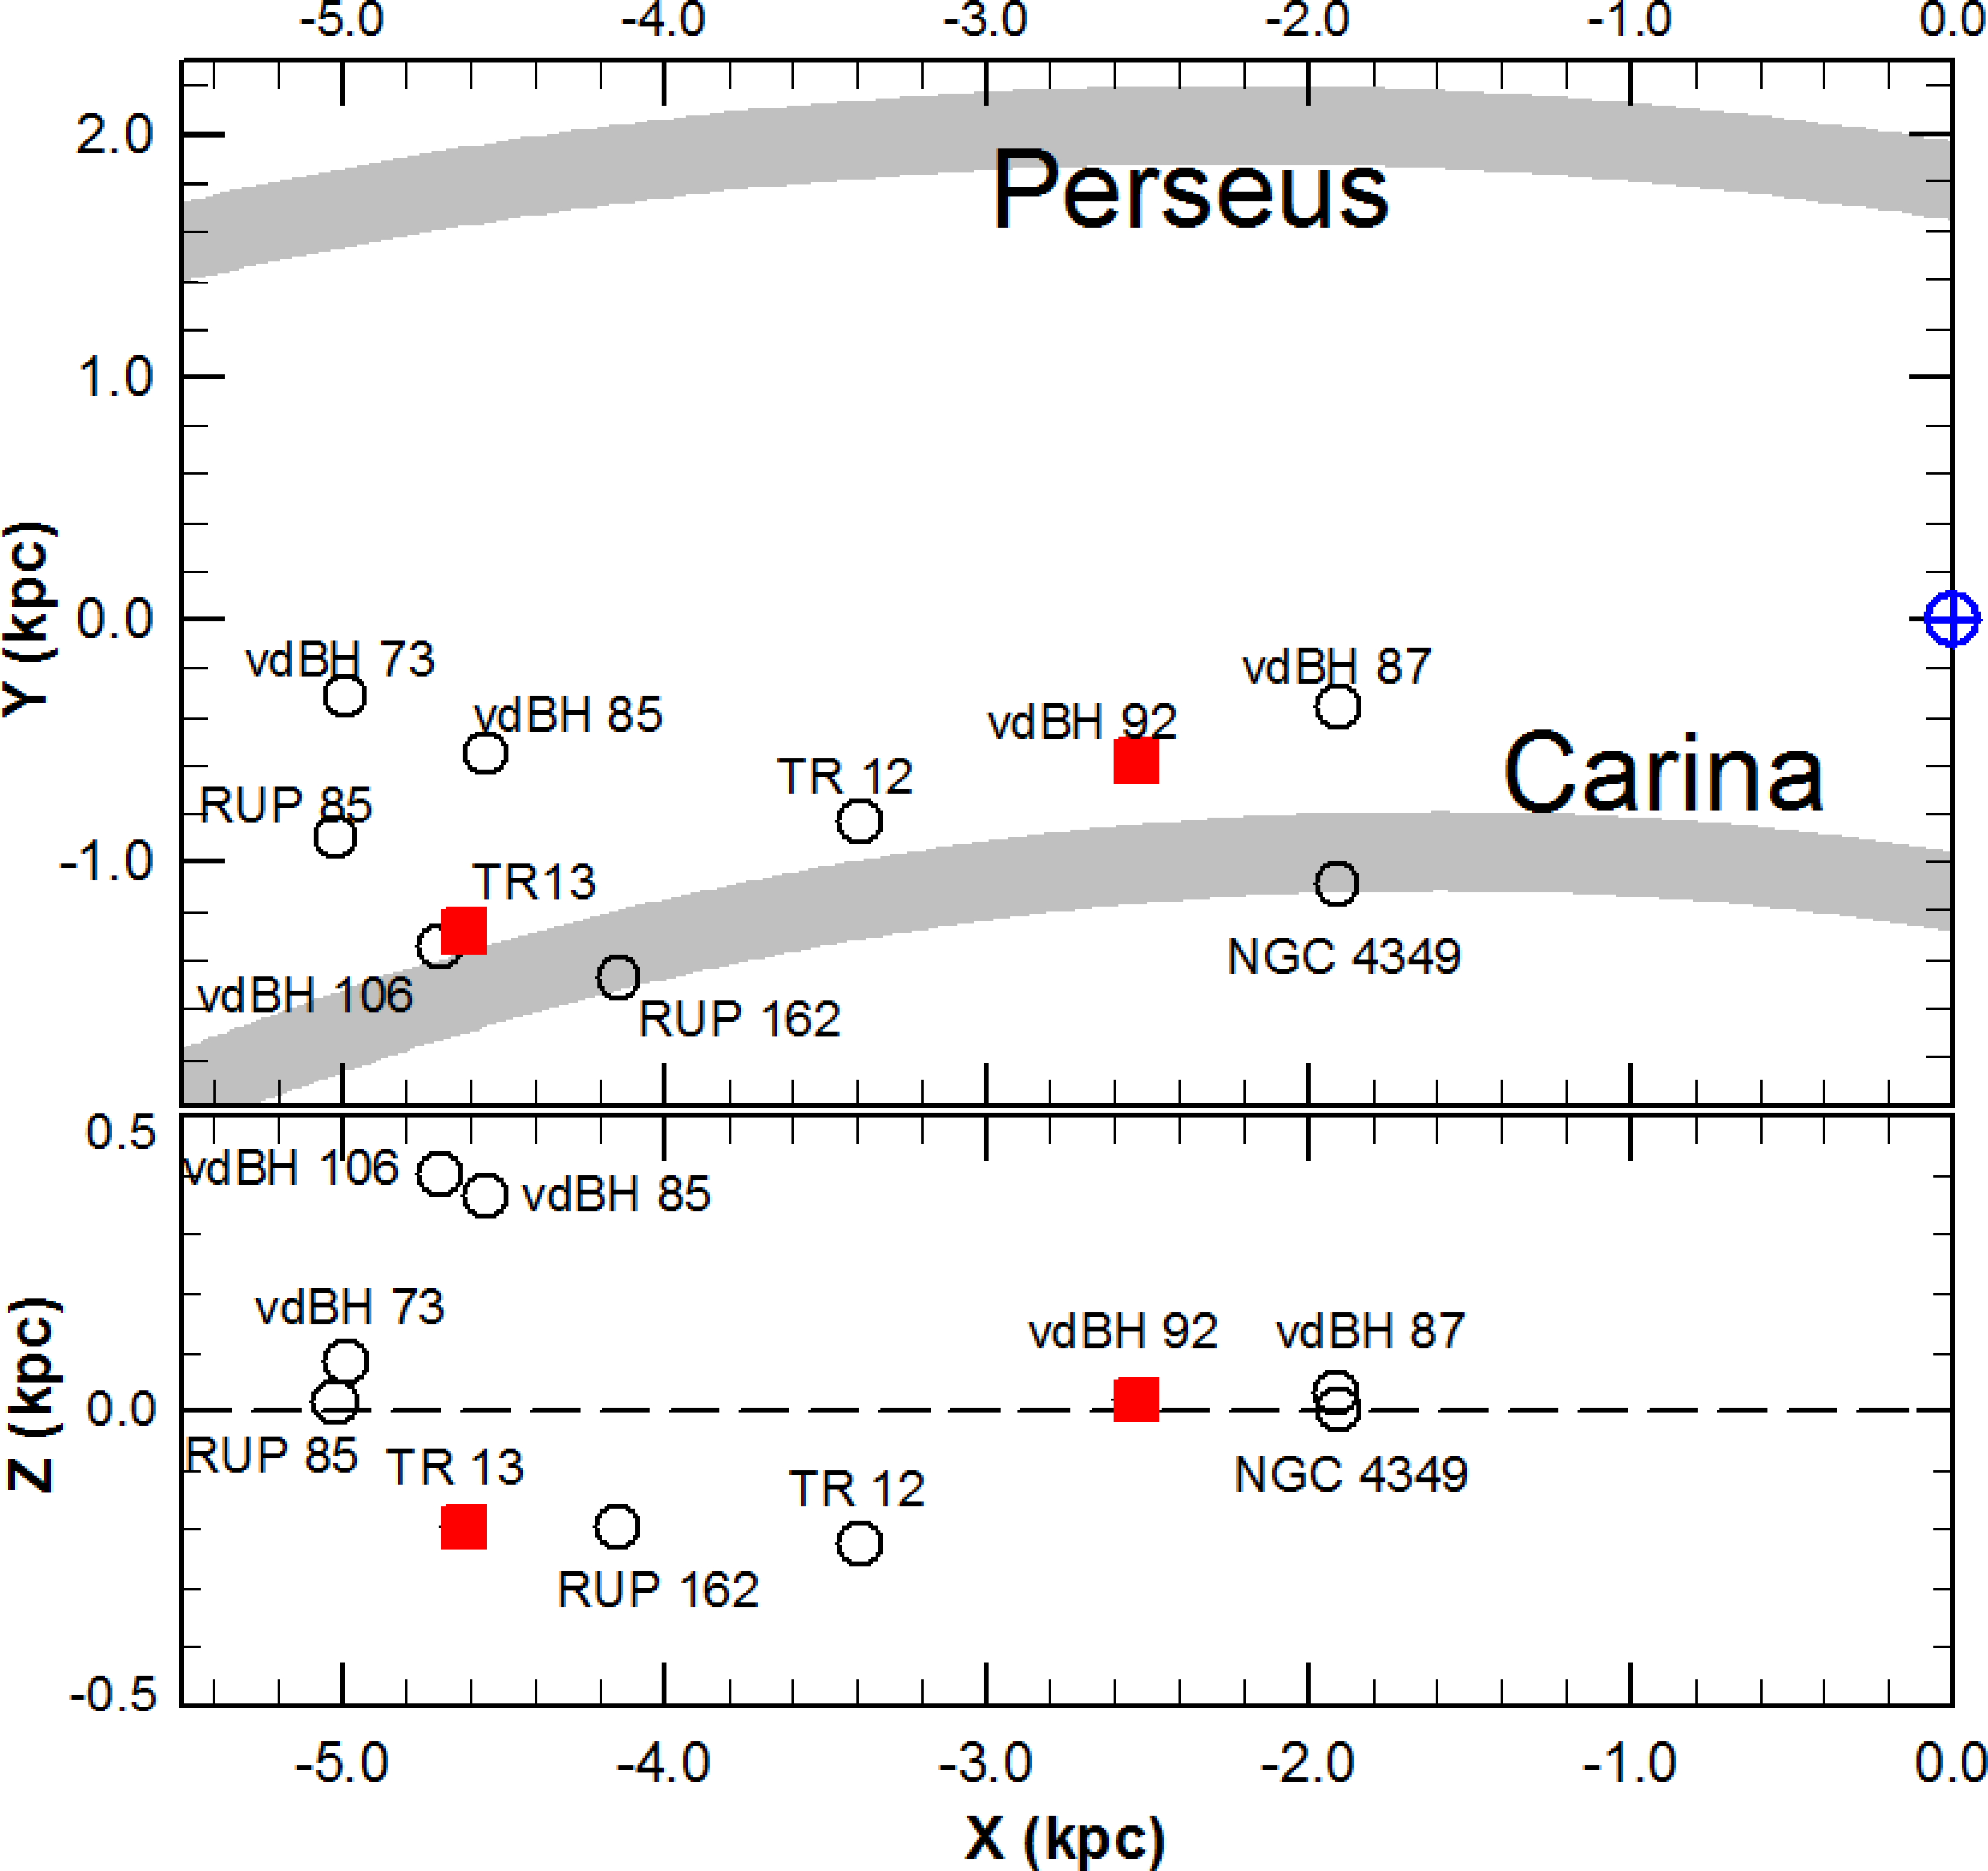
\includegraphics[width=\hsize]{figs/high_res/xy_xz.png}
    \caption{The X-Y (upper panel) and X-Z (lower plane) projection of true and
    probable clusters in our sample. In the upper panel the thick grey line
    shows the trace of Carina arm according to (XXXX) while the dashed line in
    the lower panel is for the galactic equator. Clusters displaced from 
    \texttt{ASteCA} position after adding systematic 0.1 mas to the parallaxes 
    (red dots) are joined by a line. Empty squares enclose the youngest clusters
    in our list (see Table \ref{tab:final_tab}).}
    \label{fig68}
\end{figure}

Another interesting data provided by \texttt{ASteCA} analysis is the metallicity
$z$ for each cluster included in the third column of Table \ref{tab:final_tab}.
The average value including all the clusters is $z=0.0152$ with a standard
deviation $\sigma = 0.0039$ well in agreement with modern adopted values for
solar metallicity as expected in most of open clusters.\\

There are additional reasons to be taken into account in terms of disagreements
between GAIA distances and those obtained photometrically. On one hand, 
\texttt{ASteCA} does not fit for the value of $R$ (ratio between visual
absorption and excess color, fixed at $R=3.1$) and it is known that variations
in $R$ can drastically modify distances and ages. However, these differences in
distances are very appreciable only among young clusters, but not among the
older ones. 
\texttt{ASteCA} also has some degree of difficulty in estimating the parameters
of young clusters because their main sequences are appreciably vertical and
this can introduce an appreciable fit uncertainty when there are also few
members.
This could explain the great difference with the GAIA distance that exists in
the case of RUP 162 (added to the fact that this one, in particular, may not be
a real cluster). But on the other hand, \texttt{ASteCA} fits more precisely
those clusters where there is a well defined main sequence followed by a not
ambiguous turn-off point such as the case of vdBH 73, 85, and RUP 85. And yet
the differences between photometric distances and GAIA for these objects are
among the largest. The origin of these differences may be due to offsets in
parallaxes in the regions where they are immersed.

Regarding the spiral structure in this portion of the galaxy we cannot add
much. Only three clusters are young enough to be considered spiral structure
tracers. As seen in Fig. \ref{fig68}, two of them, TR 13 and RUP 162, are
located along the Carina arm. In particular, at the distance at which TR 13 is
located, it comes to be placed 200 pc below the plane thus accompanying the
warp of this arm already mentioned by, among others, \cite{Cersosimo_2009}
A third cluster, vdBH 162, is located in an intermediate zone between the Sun
and Carina's arm. None of the objects in our sample is, therefore, related to
the arm of Perseus.


\bibliographystyle{aa}
\bibliography{biblio}


















































\appendix

The thirteen clusters in this Appendix are ordered according to their right
ascension, as shown in Table \ref{tab:clust_list}. The remaining three analyzed
clusters were presented in Sect. \ref{sec:cluster_discuss}.

%================================================================
\section{Ruprecht 85}

Ruprech 85 belongs to the south side of the Vela Constellation close to the
border of the Carina region. This cluster appears in Fig. \ref{fig2} as a slight
increment in the stellar field towards the north part in the respective frame.
The overall stars photometric diagrams as shown in Fig. \ref{fig7} do not show
the presence of any cluster sequence but a vertical strip of stars emerging from
a poorly populated stellar field above $V= 14$ mag defined by disk stars.\\

The structural analysis performed by \texttt{ASteCA} yields a clean overdensity
at the location of this object that appears subtending an almost circular area
of 3 arcmins radius, Fig. \ref{fig8} left panel. As shown in the Fig. \ref{fig8}
right panel, the RDP is well developed, scarcely noisy and with a star density
five times above the background level. The photometric diagrams, CCD and CMDs of
stars with membership probabilities above 0.6 and up to 0.99 shown in Fig.
\ref{fig9} depict a main sequence sweeping 3.5 magnitudes. Intermediate
probability members are found around the giant branch but we suggest that
care should be taken with this fact. Combining structural evidences with
evidences coming from the
photometric diagrams we conclude that RUP 85 is a real entity. As for the
cluster parameters of the best synthetic cluster fitting the observations it is
found that:

\begin{itemize}
\item [a)] Like in the case of vdBH 73, RUP 85 is also placed
    in a region of moderate color excess. In fact the cluster has $E_{(B-V)} =
    0.77$ also entirely in line with a maximum $E_{(B-V)}$ of 1.9 according to 
    S\&F2011.
\item [b)] The free absorption distance modulus is 12.67 corresponding to a
    distance $d = 3.420$ kpc.
\end{itemize}

The results from the Anderson-Darling test in Fig. \ref{fig10} applied to $Plx$,
$PM(\alpha)$ and $PM(\delta)$ indicate clearly that the cluster region and the
surrounding background population come from quite different star populations.
Therefore, the null hypothesis can be rejected.\\

We conclude that RUP 85 is a real open cluster over $891\times10^6$ yr old.

\begin{figure*}[ht]
    \centering
    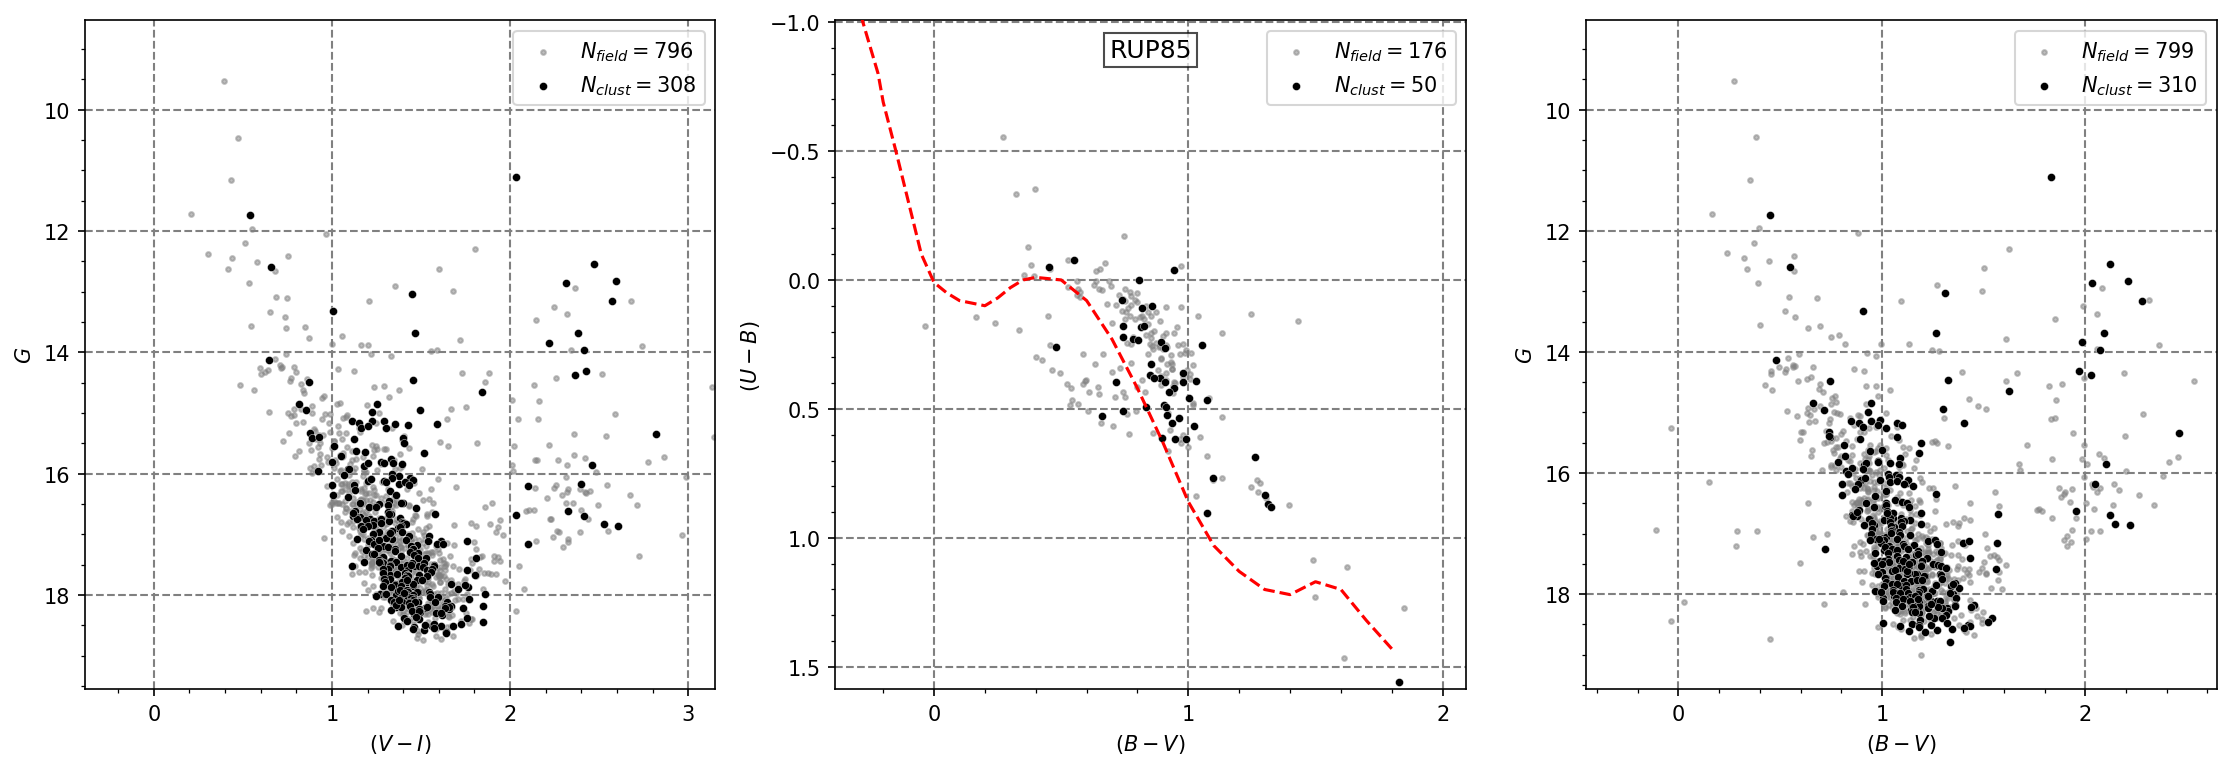
\includegraphics[width=\hsize]{figs/high_res/obs_RUP85.png}
    \caption{Idem Fig. \ref{fig3} for RUP 85.}
    \label{fig7}
\end{figure*}

\begin{figure*}[ht]
    \centering
    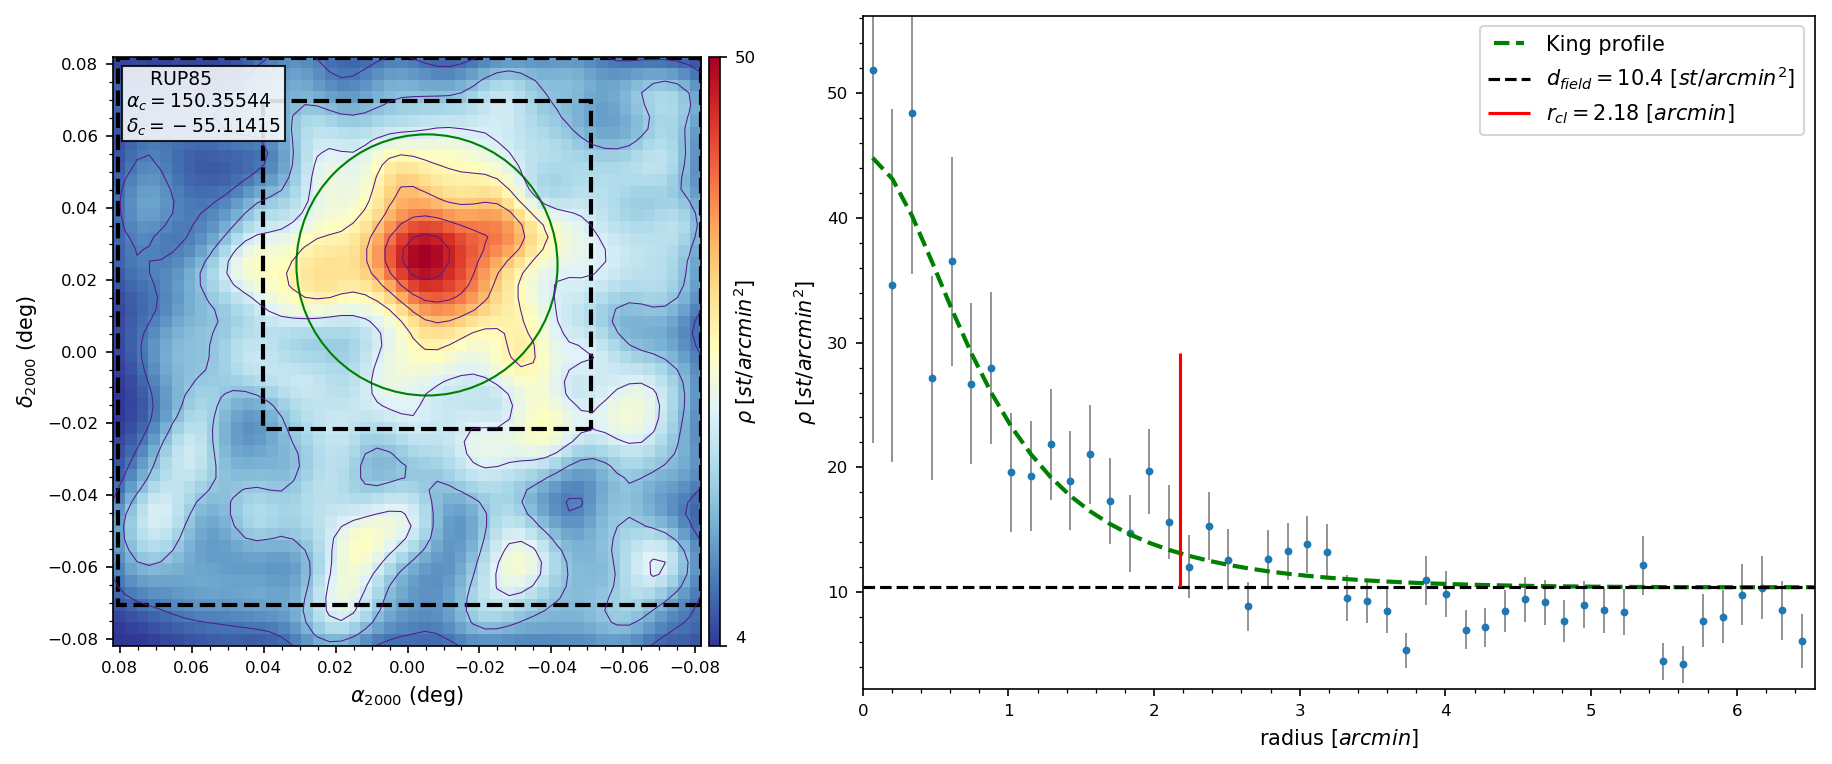
\includegraphics[width=\hsize]{figs/high_res/dmap_rup85.png}
    \caption{Idem Fig. \ref{fig4} for RUP 85.}
    \label{fig8}
\end{figure*}

\begin{figure*}[ht]
    \centering
    \includegraphics[width=\hsize]{figs/high_res/cmds_rup85.png}
    \caption{Idem Fig. \ref{fig5} for RUP 85.}
    \label{fig9}
\end{figure*}

\begin{figure*}[ht]
    \centering
    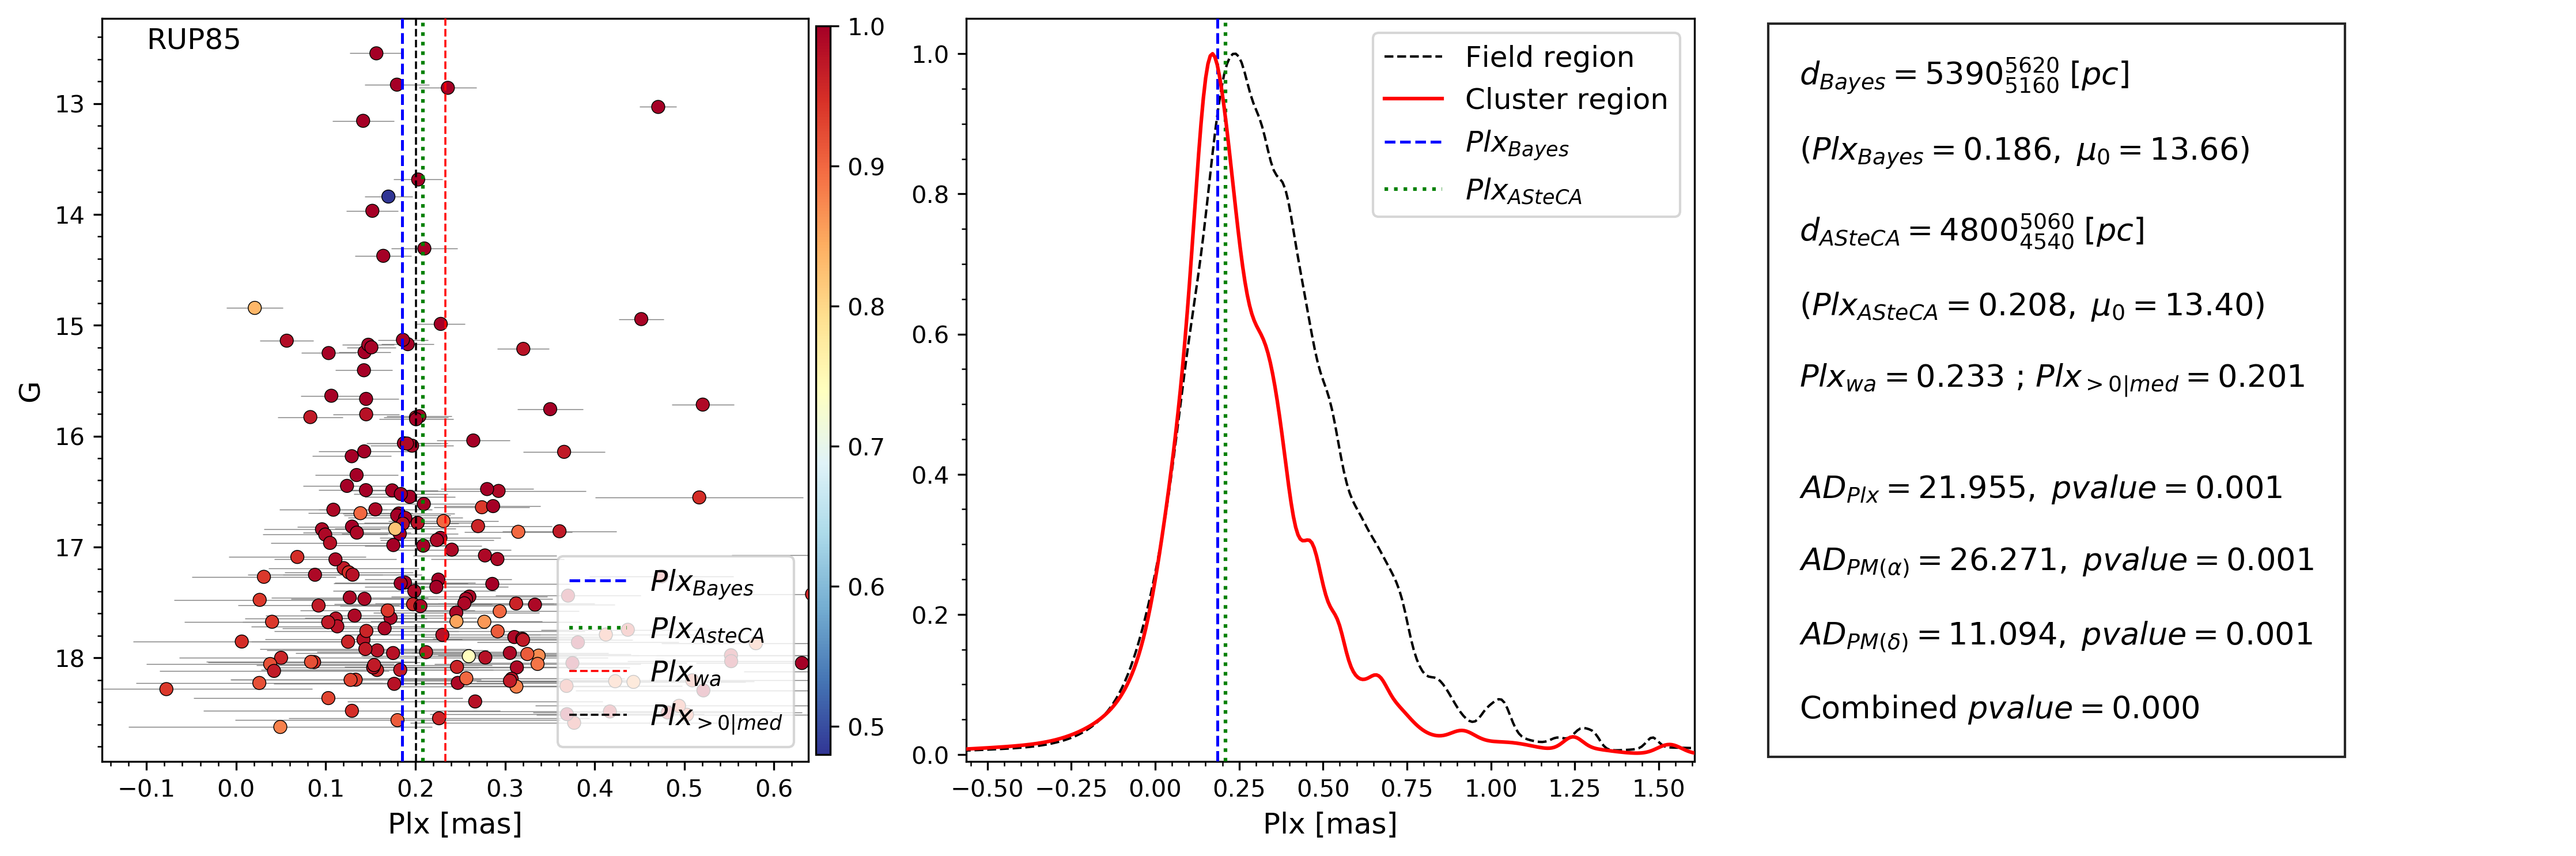
\includegraphics[width=\hsize]{figs/high_res/plx_RUP85.png}
    \caption{Idem Fig. \ref{fig6} for RUP 85.}
    \label{fig10}
\end{figure*}



%================================================================
\section{van den Bergh-Hagen 85}

vdBH 85 appears in the sky slightly east of the center of the
Vela constellation. The $V$ chart in Fig. \ref{fig2} shows a weak star
concentration near the north side of the observed field extending a little bit
to the south east. The photometric diagrams of the entire field of view is just
a dispersed star distribution ending in a compact accumulation at $(B-V)=1$ and
below $V = 17$ mag approximately. Another clear feature in the two CMDs is a
structure at $V = 16$ and for $1.2 < (B-V) < 1.7$ resembling a red clump.\\

\texttt{ASteCA} detected an overdensity very well detached from the stellar
background reflected in the smooth RDP in Fig. \ref{fig12} contained in a circle
2.8 arcmins radius and more than five times the background density. Once the
removal of field interlopers is done and the membership probabilities are
established the two CMDs of all stars with probabilities above 0.56 show a short
but evident main sequence below $V = 17$ mag. Three magnitudes above the cluster
turn-off, at $V = 14$ mag two stars appear. Since they have large membership
probability, near 0.87, they could be blue straggler associated to van den
Bergh-Hagen 85. There is in the bright end of the giant branch two other stars
with more than 0.8 membership probability that reinforces the real existence of
a giant branch. The comparison with the best fitting of a synthetic cluster
throws the following characteristics for vdBH 85:

\begin{itemize}
\item [a)] the cluster is seen projected against a stellar field with moderate to
    low color excess. The best value corresponds to $E_{(B-V)} = 0.34$ in
    correspondence with the maximum value of 0.45 stated by S\&F2011.
\item [b)] The free absorption distance modulus of vdBH 85 is
    13.14 what implies a distance of 4.246 kpc from the Sun. This fact explains
    by itself the extreme weakness of cluster members.
\end{itemize}

The Anderson-Darling test results in Fig. \ref{fig14} suggest the impossibility
to accept the null hypothesis valid. In fact, $Plx$, $PM(\alpha)$ and
$PM(\delta)$ results from the Anderson-Darling test leave no doubt in the sense
that cluster region and the surrounding comparison field come from quite
different star populations.\\

We conclude that this object is a real cluster approximately $5011\times10^6$
yrs old.

\begin{figure*}[ht]
    \centering
    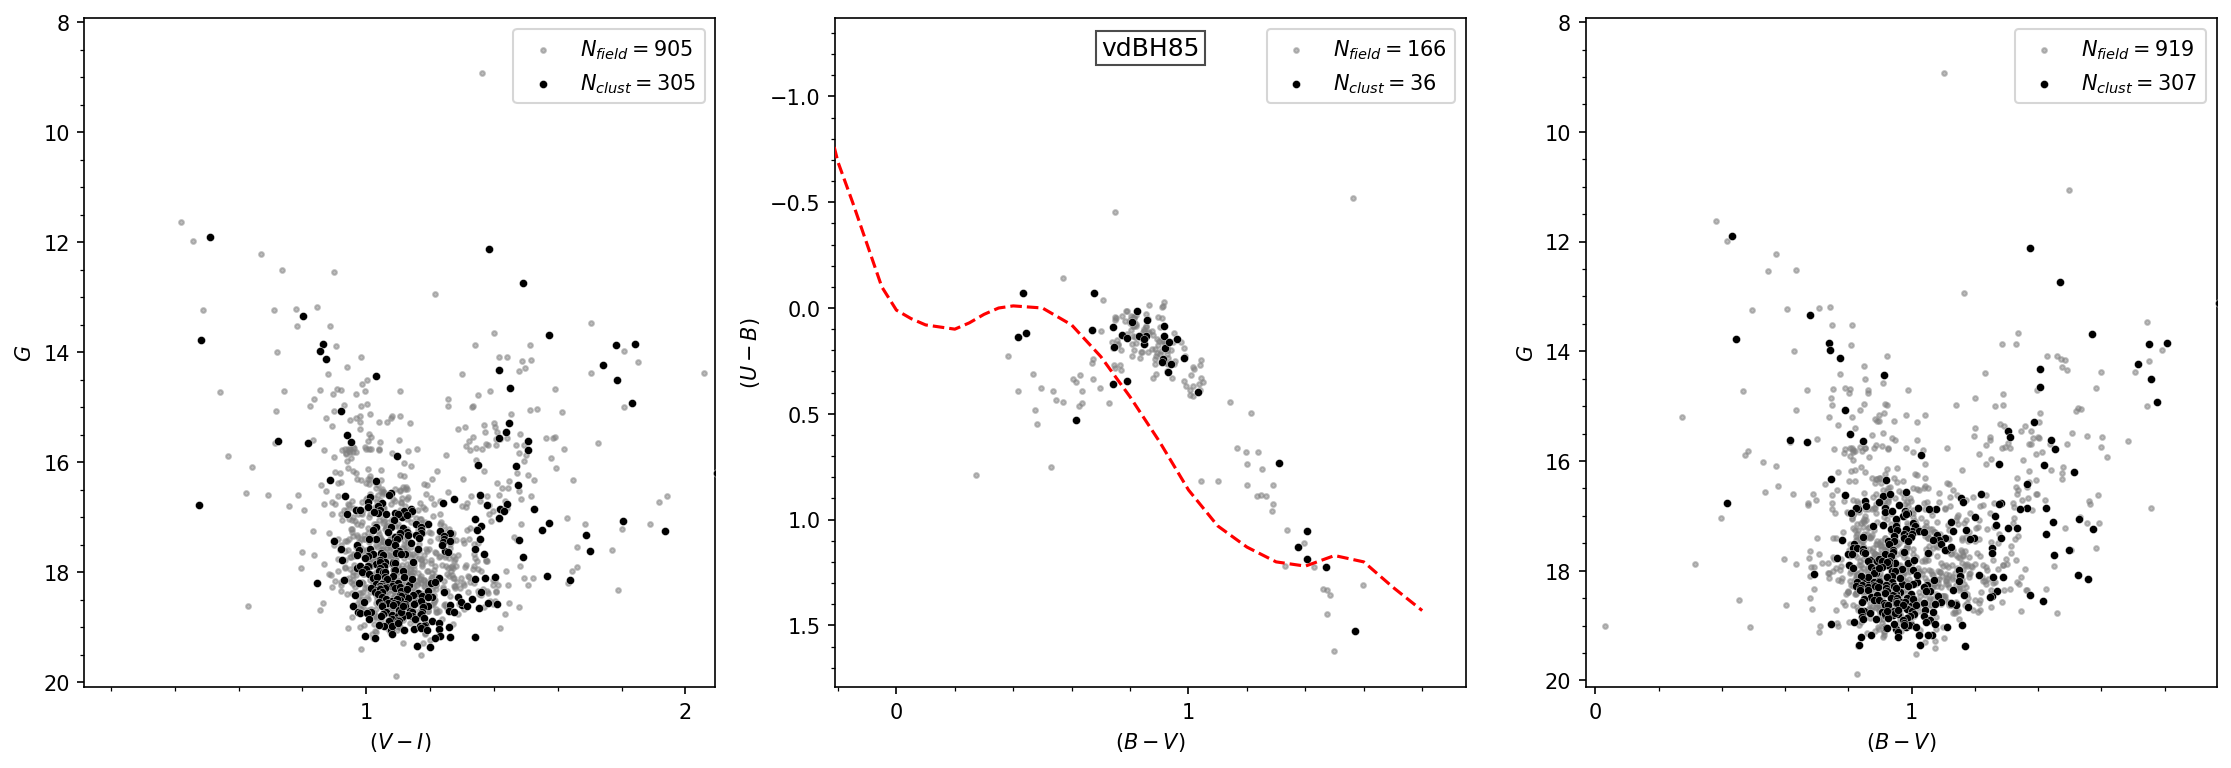
\includegraphics[width=\hsize]{figs/high_res/obs_vdBH85.png}
    \caption{Idem Fig. \ref{fig3} for vdBH 85.}
    \label{fig11}
\end{figure*}

\begin{figure*}[ht]
    \centering
    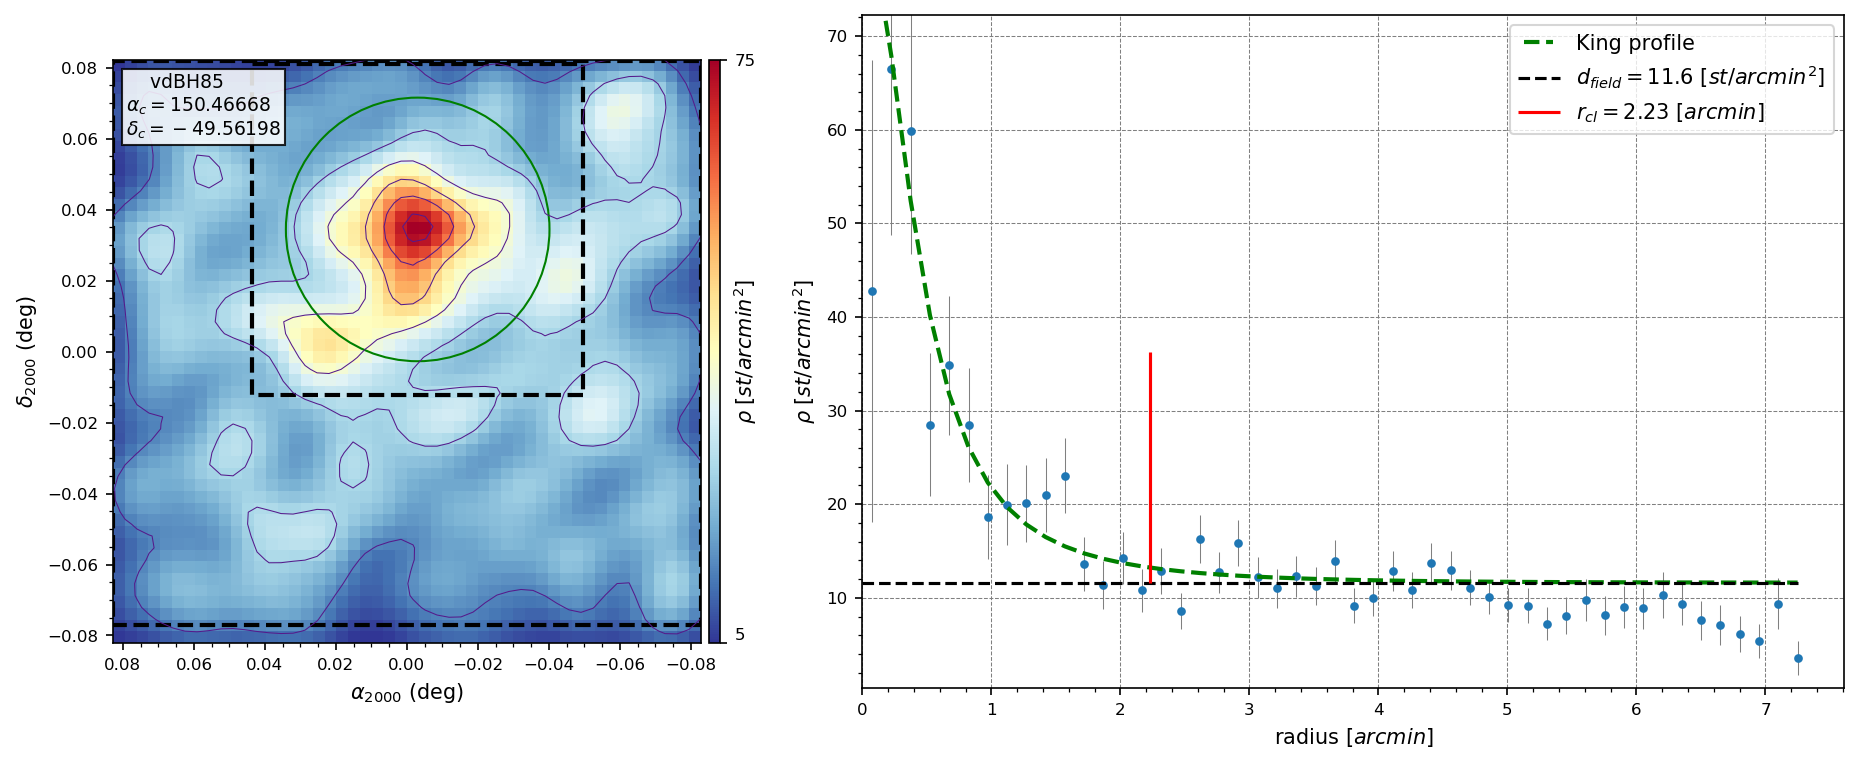
\includegraphics[width=\hsize]{figs/high_res/dmap_vdbh85.png}
    \caption{Idem Fig. \ref{fig4} for vdBH 85.}
    \label{fig12}
\end{figure*}

\begin{figure*}[ht]
    \centering
    \includegraphics[width=\hsize]{figs/high_res/cmds_vdbh85.png}
    \caption{Idem Fig. \ref{fig5} for vdBH 85.}
    \label{fig13}
\end{figure*}

\begin{figure*}[ht]
    \centering
    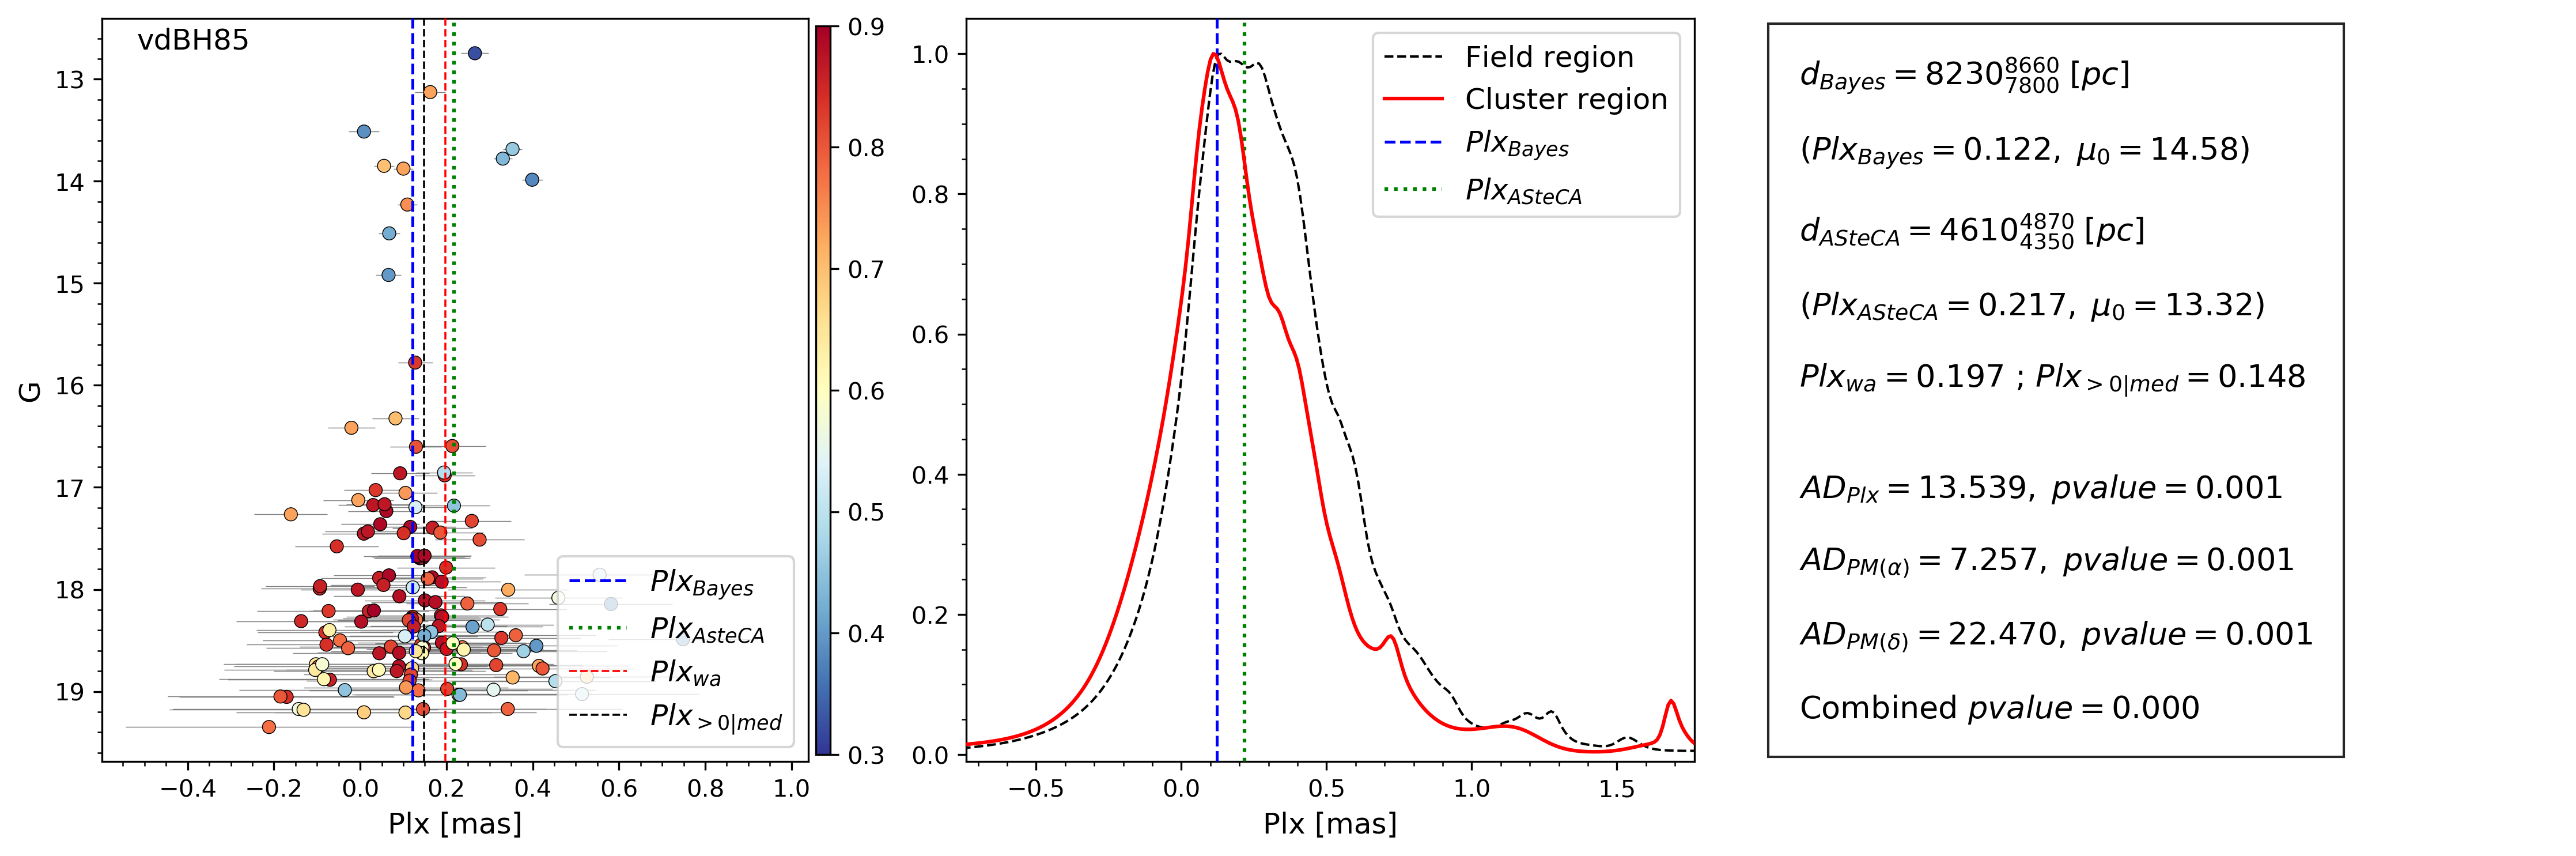
\includegraphics[width=\hsize]{figs/high_res/plx_vdBH85.png}
    \caption{Idem Fig. \ref{fig6} for vdBH 85.}
    \label{fig14}
\end{figure*}



%================================================================
\section{van den Bergh-Hagen 87}

Like RUP 85, vdBH 87 is seen toward the south of Vela
Constellation close to the border with Carina. A weak grouping of stars placed
towards the north of the frame is seen in Fig. \ref{fig2}. In turn, the CMDs in
Fig. \ref{fig15} seem to reflect a typical star disk sequence up to $V = 15$ mag
approximately with an amorphous distribution at the bright end. The CCD is, on
the other side, rather poor.\\

A stellar overdensity reaching $\sim20$ times the field star density is
seen in Fig. \ref{fig16}. The spatial structure of this overdensity suggests an
elongation in right ascension and a RDP characterized by a very narrow density
peak followed by a star coronal distribution at about 2 arcmins from the center.
The clean CMDs in Fig. \ref{fig17} leave no doubt as for the nature of van den
Bergh-Hagen 87 since inside this overdensity a robust and narrow cluster main
sequence is evident. It extends for more than 5 mag including stars with
membership probabilities in the range from 0.54 to 1. A few stars with high
membership probability have been found in the CCD following the same trend for
reddening. The parameters of the synthetic cluster that best fits the real star
distributions are:

\begin{itemize}
\item [a)] The color excess is $E_{(B-V)} = 0.56$ indicating thus a moderate
    absorption in the cluster direction. In turn, this color excess value is
    below the maximum reddening $E_{(B-V)} = 2.9$ computed in the region for 
    S\&F2011.
\item [b)] The corrected distance modulus is 11.4 implying a distance of $d =
    1.905$ kpc. The cluster is not far from the Sun and this closeness explains
    the moderate color excess found.
\end{itemize}

The results of the application of the Anderson-Darling test in Fig. \ref{fig18}
are coincident with what \texttt{ASteCA} have found. This is that cluster and
field regions are quite different not only from the photometric perspective but
also from a kinematic view.\\

In conclusion vdBH 87 is a real open cluster about
$630\times10^6$ years old.

\begin{figure*}[ht]
    \centering
    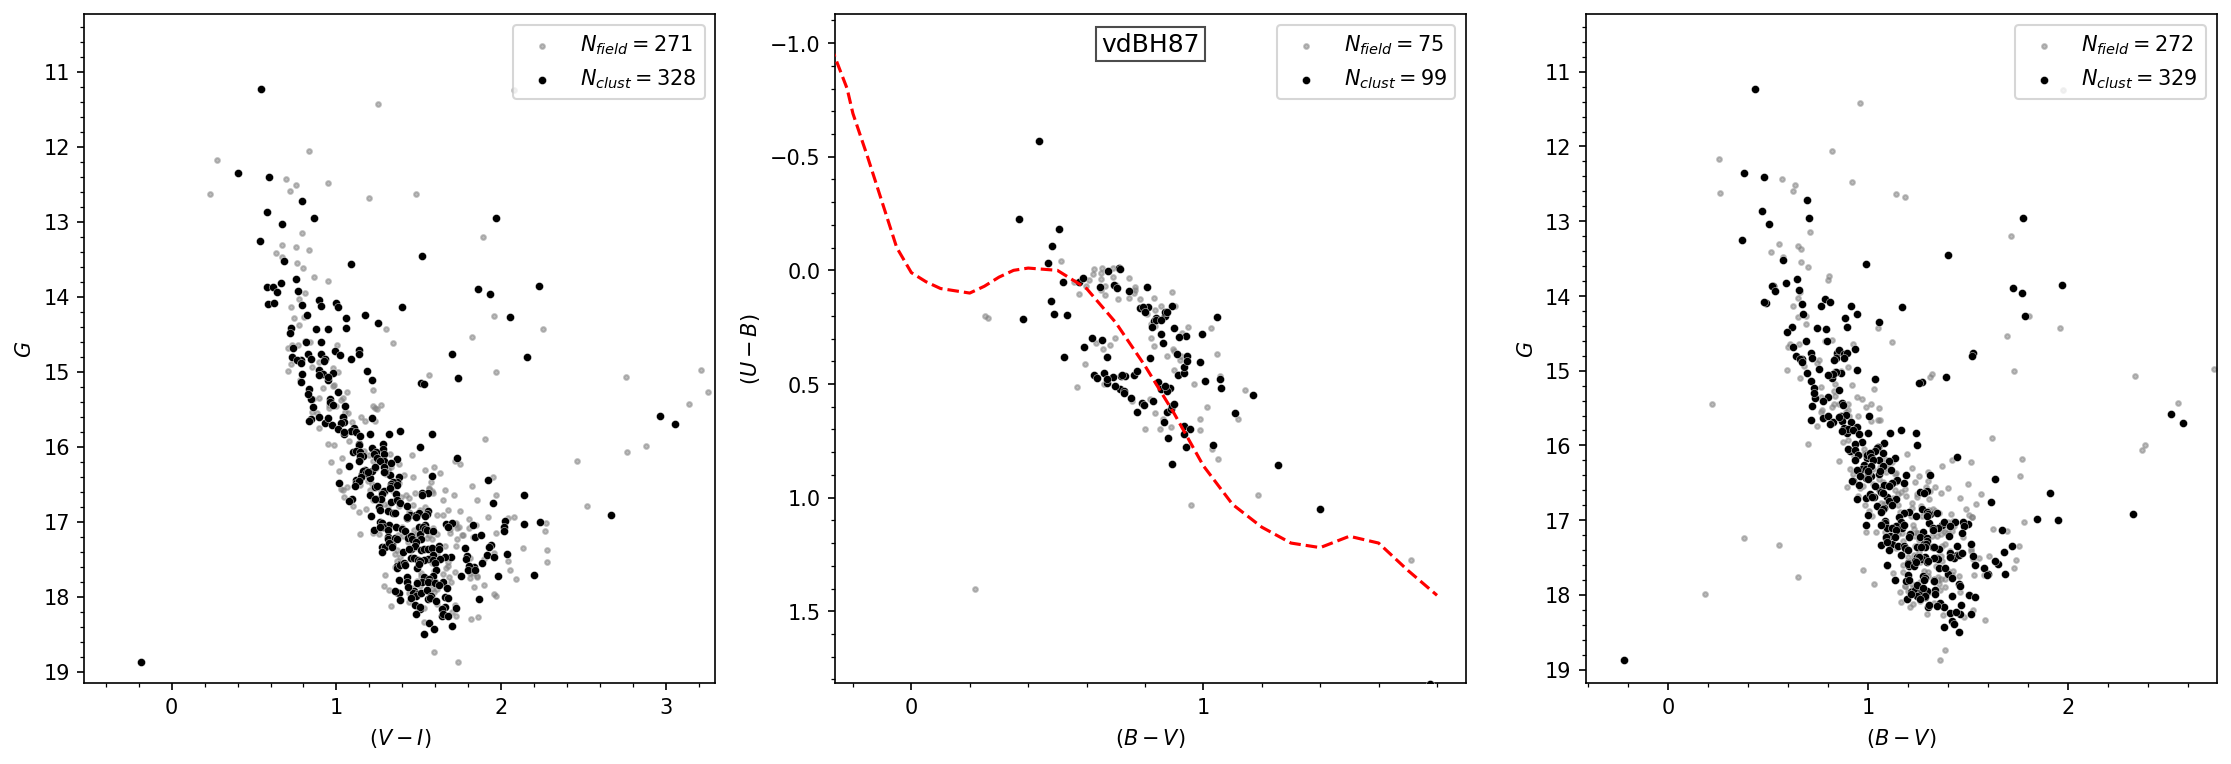
\includegraphics[width=\hsize]{figs/high_res/obs_vdBH87.png}
    \caption{Idem Fig. \ref{fig3} for vdBH 87.}
    \label{fig15}
\end{figure*}

\begin{figure*}[ht]
    \centering
    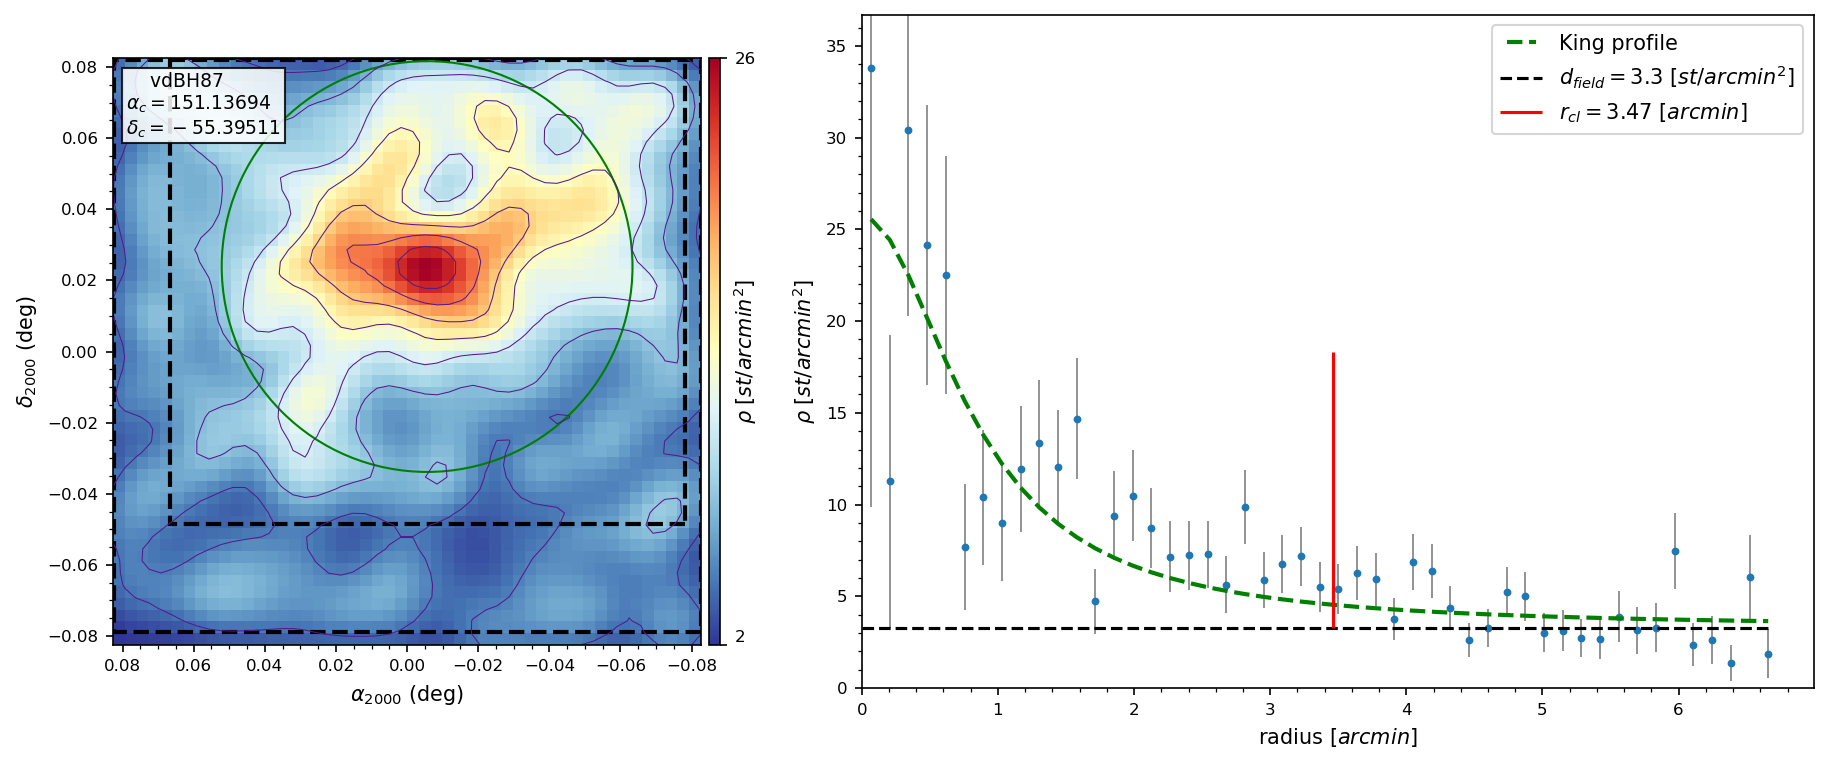
\includegraphics[width=\hsize]{figs/high_res/dmap_vdbh87.png}
    \caption{Idem Fig. \ref{fig4} for vdBH 87.}
    \label{fig16}
\end{figure*}

\begin{figure*}[ht]
    \centering
    \includegraphics[width=\hsize]{figs/high_res/cmds_vdbh87.png}
    \caption{Idem Fig. \ref{fig5} for vdBH 87.}
    \label{fig17}
\end{figure*}
\begin{figure*}[ht]
    \centering
    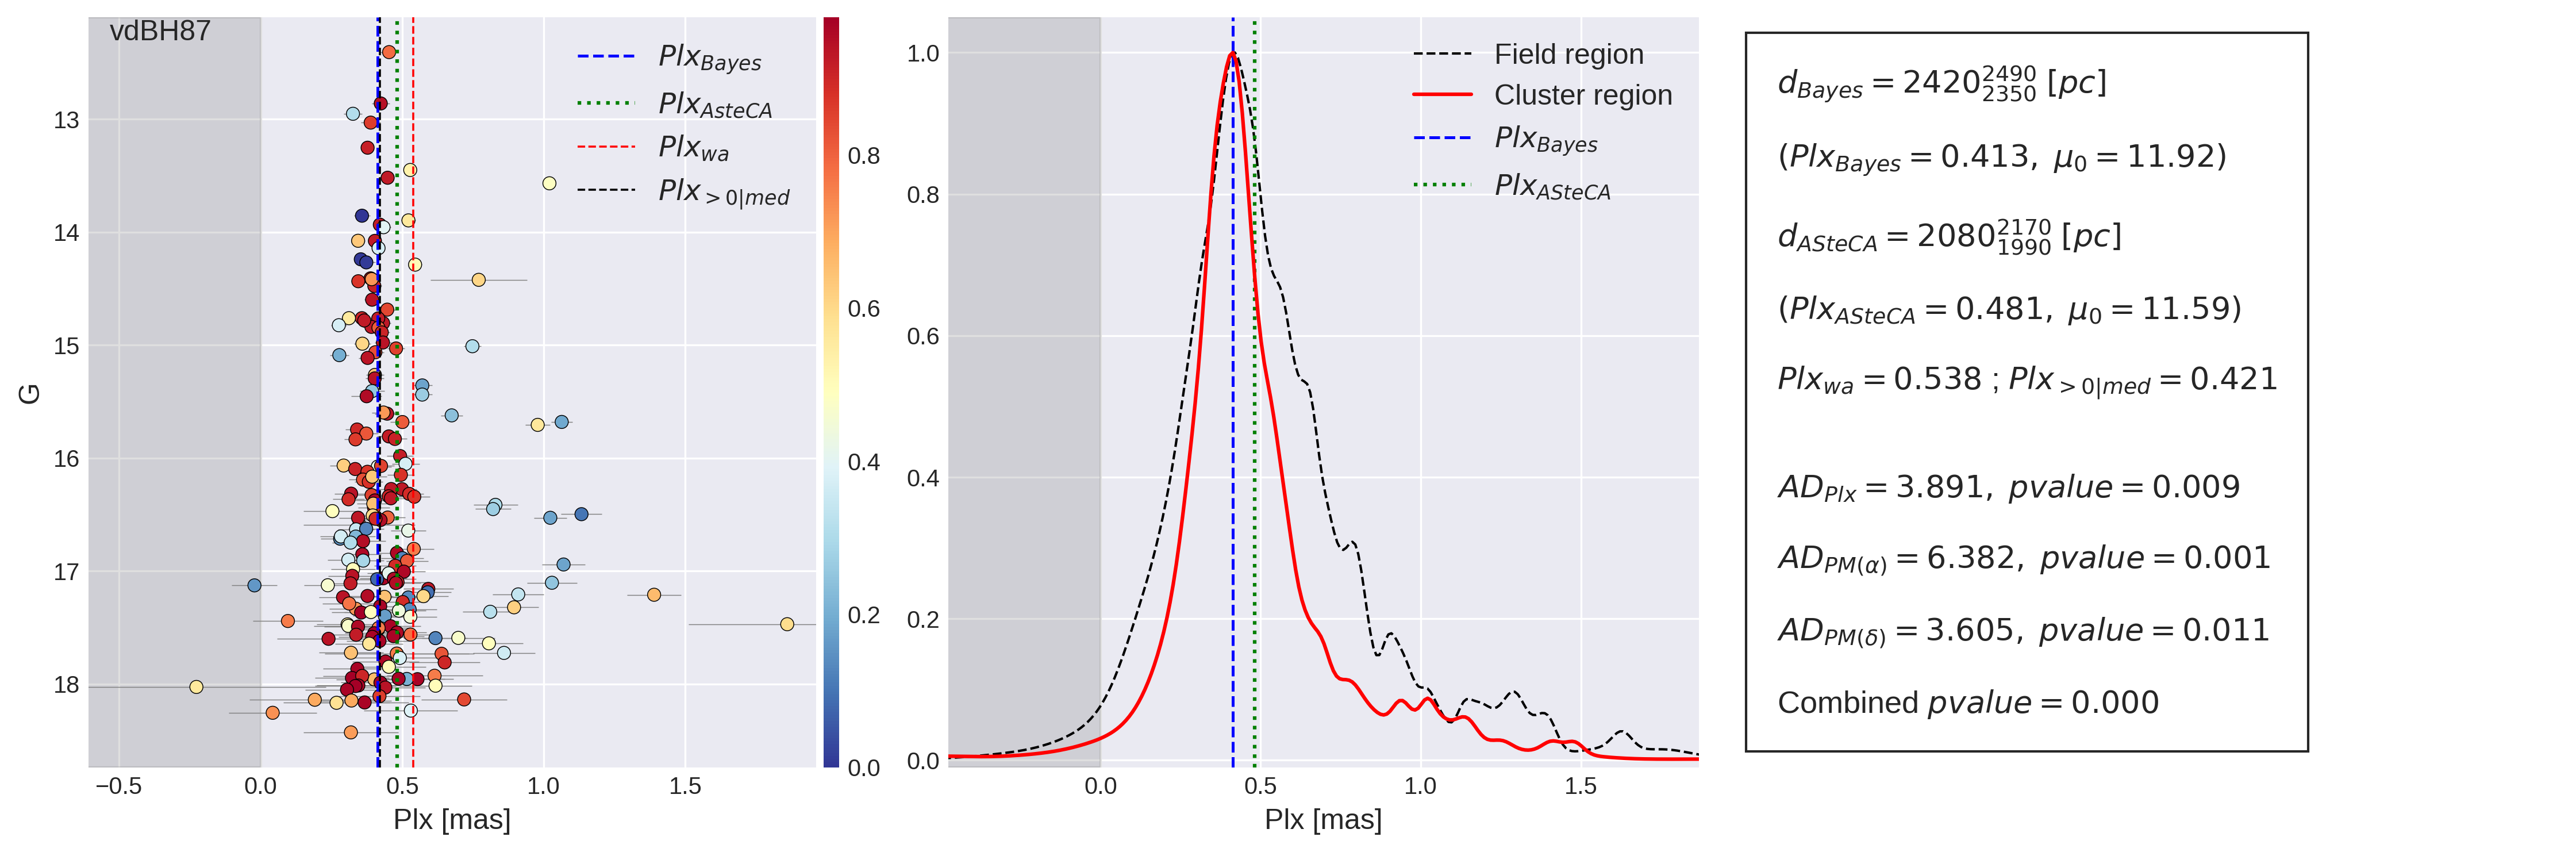
\includegraphics[width=\hsize]{figs/high_res/plx_vdBH87.png}
    \caption{Idem Fig. \ref{fig6} for vdBH 87.}
    \label{fig18}
\end{figure*}




%================================================================
\section{Trumpler 12}

This object is placed in the west side of the Carina HII region where it appears
as a sparse handful of bright stars in Fig. \ref{fig2}. The CMDs in Fig.
\ref{fig19}, including all stars in the region, show the following patterns:
there is a wide grouping of stars below $V = 18$ mag but to the right side of
it, and also at this magnitude value, a narrow structure of stars up to $V= 14$
mag slightly displaced to the blue side emerges. From $V = 18$ mag a typical
vertical galactic disk population rises too.\\

\texttt{ASteCA} detected a main overdensity and other less relevant ones shown
in Fig. \ref{fig20}. The reader can note a quite noisy RDP, a fact explained in
part because at the peak of the RDP there is less than twice the density of the
background. Under this condition is not an easy task to fix an appropriate
radius for the overdensity. We tentatively adopt 3 arcmin radius as a reasonable
compromise. The membership probabilities in the zone of the overdensity range
from 0.35 to 0.71 as indicated in Fig. \ref{fig21}. We draw the attention to the
fact that only 126 stars were detected inside the potential cluster zone. These
values indicate the obvious difficulty to separate field stars from cluster
members since most of the stars below V= 16 mag may equally belong to the
cluster or to the stellar background field. For smaller magnitudes the
probabilities slightly increase and some stars describe roughly a cluster main
sequence. In particular some of them belonging to the tiny blue and narrow
sequence detected easily in the diagrams of Fig. \ref{fig19} form part
(including the turn-off stars) of the clean sequence between $V = 12$ and $V =
16$ mag seen in Fig. \ref{fig21}. Comparison with synthetic clusters is still
possible and the properties of the best fit achieved in the present case are the
next:

\begin{itemize}
\item [a)] A color excess of $E_{(B-V)} = 0.26$ is found for the best fitting.
    Since the maximum color excess provided by S\&F2011 is 0.50 we found a
    precedent result and in case TR 12 is a real cluster it is placed in a
    zone of low absorption.
\item [b)] The absorption free distance modulus becomes 12.42 representing a
    distance of 3.048 kpc. At such a distance and with low absorption it is
    reasonable to find a high background stellar density as seen in Fig. 
    \ref{fig20}.
\end{itemize}

It is evident, from the Anderson-Darling statistics shown in Fig. \ref{fig21}
that mean parallaxes and proper motions for the cluster and for the field
population belong to different samples.\\

The low probabilities for all the stars inside the overdensity, the noisy
profile that does not allow establishing a clear cluster extension and the poor
main sequence requires us to be cautious. More deep photometry ($(U-B)$
particularly) is needed to achieve a precise result as for the true nature of
this object. Meanwhile we conclude that TR 12 is a dubious cluster about
$446\times10^6$ years.

\begin{figure*}[ht]
    \centering
    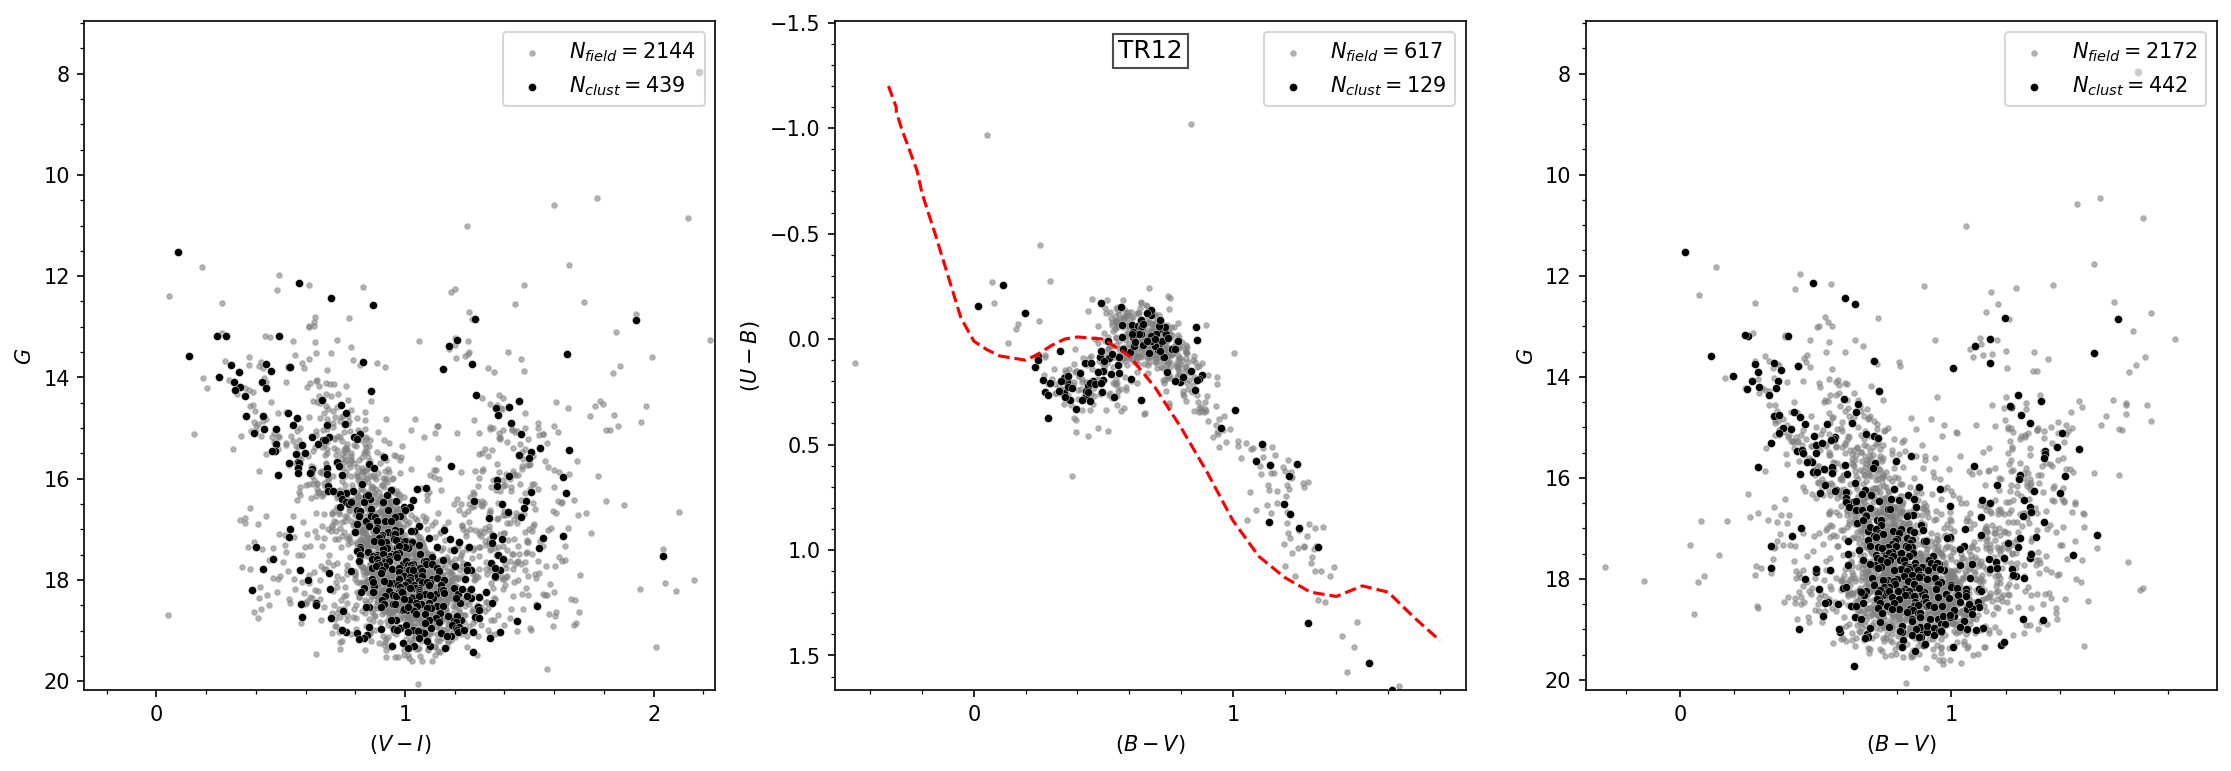
\includegraphics[width=\hsize]{figs/high_res/obs_TR12.png}
    \caption{Idem Fig. \ref{fig3} for TR 12.}
    \label{fig19}
\end{figure*}
\begin{figure*}[ht]
    \centering
    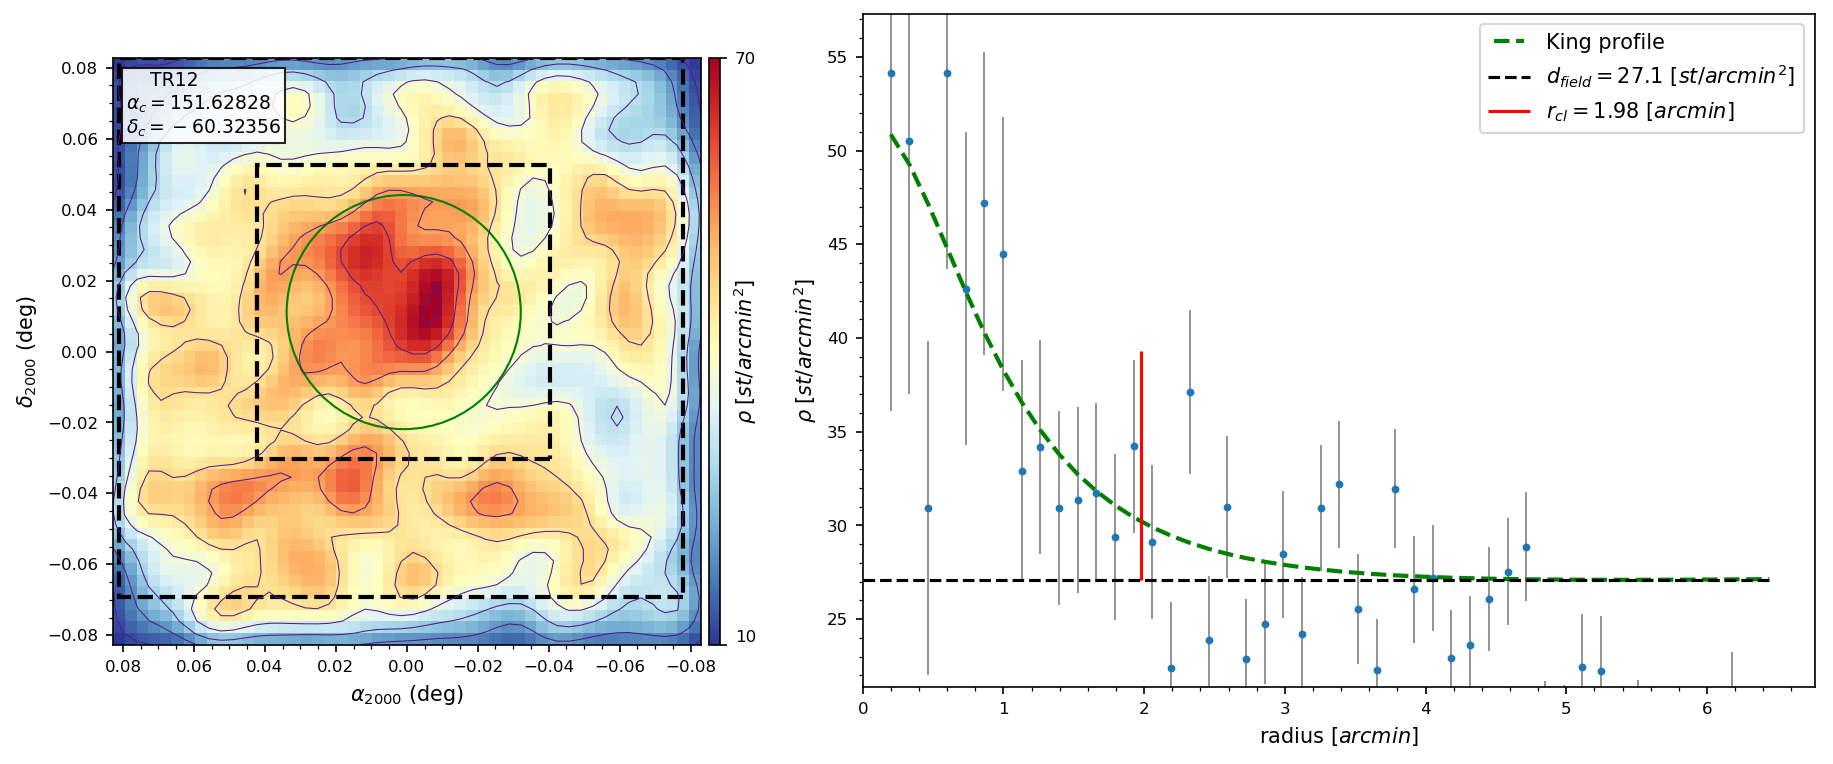
\includegraphics[width=\hsize]{figs/high_res/dmap_trumpler12.png}
    \caption{Idem Fig. \ref{fig4} for TR 12.}
    \label{fig20}
\end{figure*}
\begin{figure*}[ht]
    \centering
    \includegraphics[width=\hsize]{figs/high_res/cmds_tr12.png}
    \caption{Idem Fig. \ref{fig5} for TR 12.}
    \label{fig21}
\end{figure*}
\begin{figure*}[ht]
    \centering
    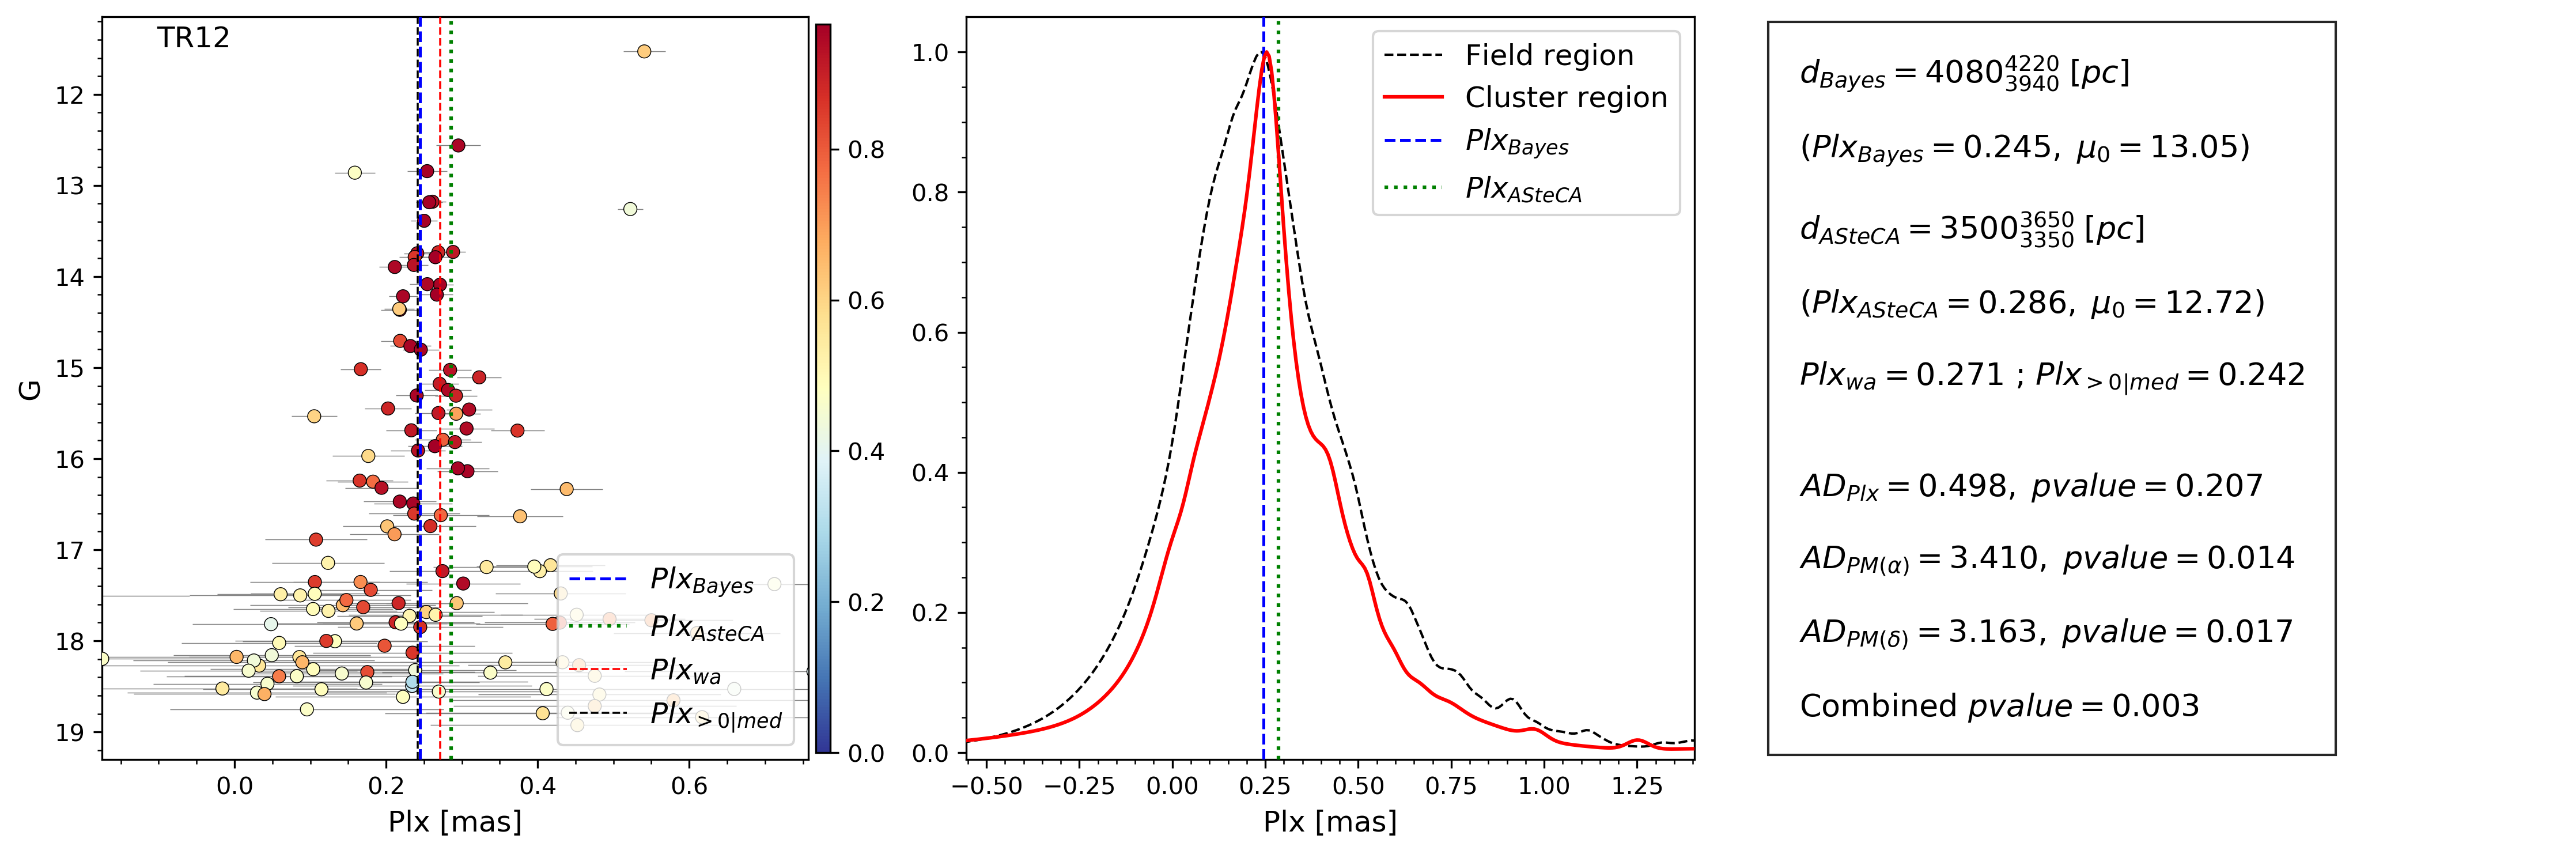
\includegraphics[width=\hsize]{figs/high_res/plx_TR12.png}
    \caption{Idem Fig. \ref{fig6} for TR 12.}
    \label{fig22}
\end{figure*}



%================================================================
\section{van den Bergh-Hagen 91}

vdBH 91 is a potential cluster at the west side of Carina HII
region, specifically near the northern border of this constellation with Vela.
No relevant stellar structure appears in the $V$ image of Fig. \ref{fig2} but a
common pattern of a galactic field star near the galactic plane. The overall
CMDs in Fig. \ref{fig27} show a stellar sequence that, at first sight, resemble
the usual diagrams for open clusters. In turn, the CCD
is dominated by a tail of $F$- and $G$-type stars prolonged by red stars. It is
noticed as well the presence of some reddened early type stars for negative
$(U-B)$ indices.\\

\texttt{ASteCA} found two well separated stellar overdensity peaks in Fig.
\ref{fig28} whose relevance in terms of stellar density is barely important
since they include no more than three stars above the background density. The
noisy RDP proves by itself the poverty of the entire field surveyed in term of
star number. After some attempts looking for a cluster sequence we ask
\texttt{ASteCA} to estimate the probabilities for stars inside an adopted radius
of 3.6 arcmin shown in Fig. \ref{fig28} right. As seen in Fig. \ref{fig29} a
hundredth of stars inside the circle associated to vdBH 91 has
been found in the CMDs with membership probabilities ranging from 0.37 to 0.79.
It is interesting that most stars with lower probabilities outline a fictitious
sequence below $V = 16$ mag in these diagrams while stars with higher
probabilities are scattered between the location of a probable main sequence and
a giant stars branch. So, the absence of a cluster sequence combined with the
poor and noisy overdensity is all against the reliability of this cluster. The
Anderson-Darling test in Fig. \ref{fig30}, right panel, is clear regarding the
true nature of vdBH 91 since the high combined $p$-value
indicates that the null hypothesis (cluster and field areas come from the same
originating distribution) con not be reasonably rejected. This result is against
the \cite{Kharchenko_2005} findings who found
that vdBH 91 is a cluster at 0.740 kpc, $160\times10^6$ yr old
approximately and affected by a mean color excess $E_{(B-V)} = 0.08$.\\

We conclude that vdBH 91 is a random fluctuation of the stellar
background instead of a real entity.

\begin{figure*}[ht]
    \centering
    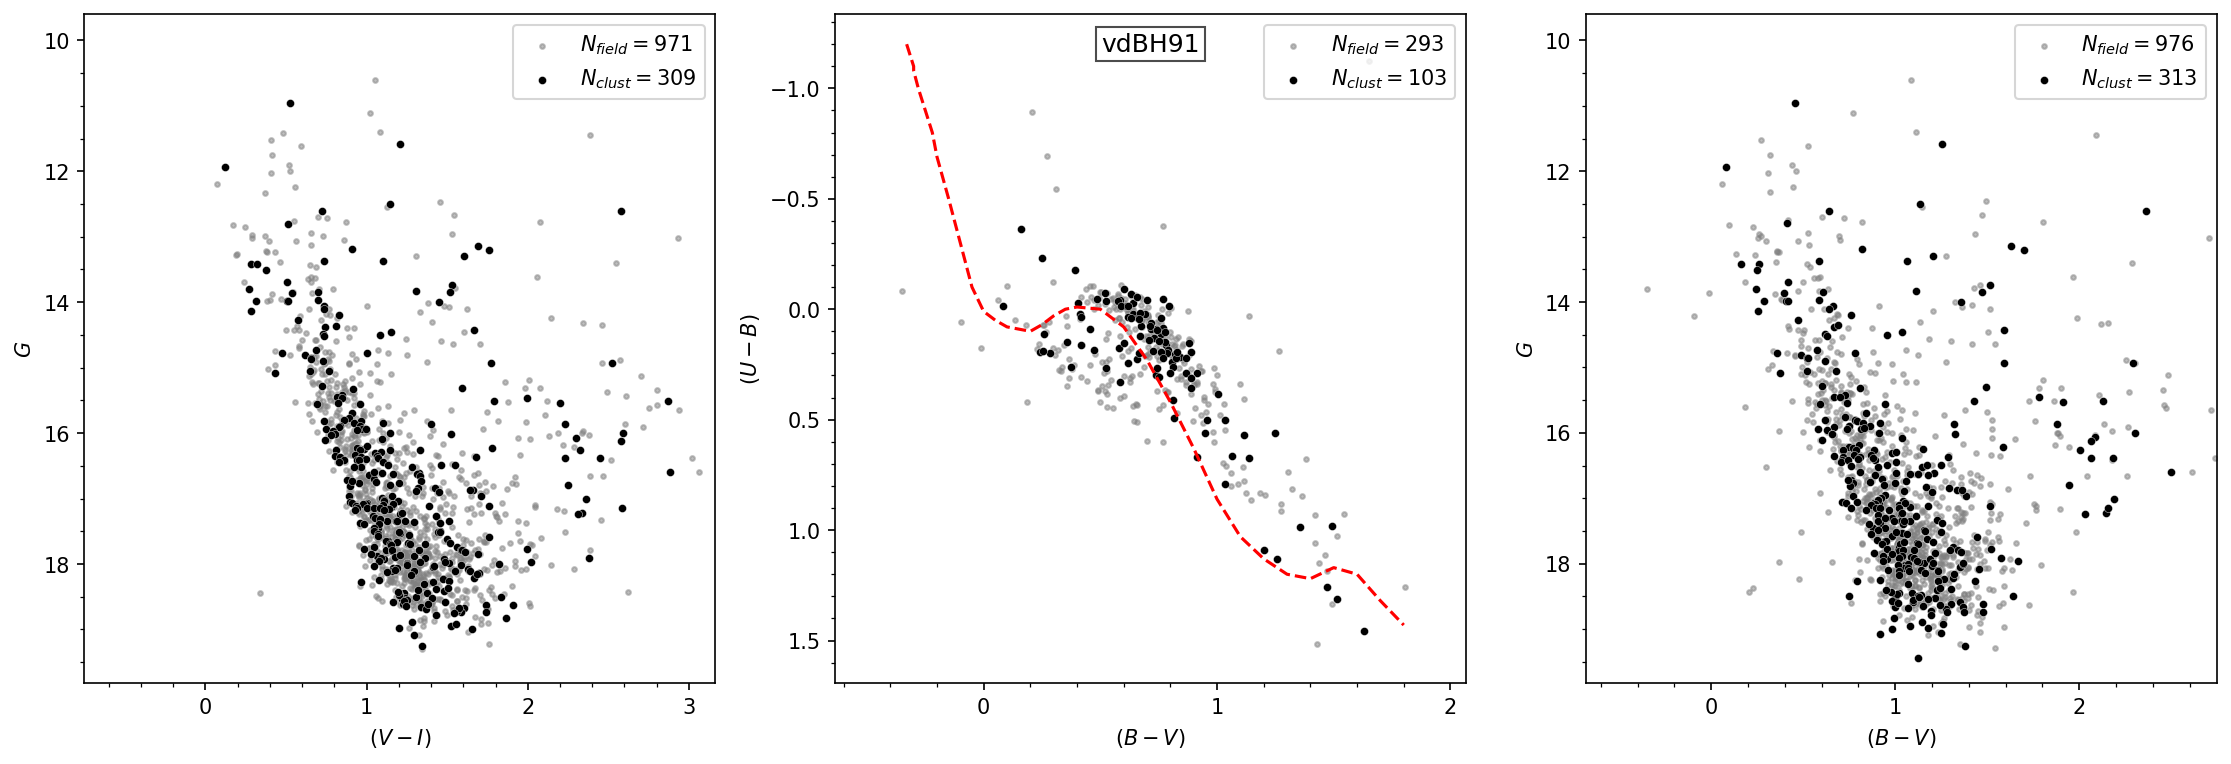
\includegraphics[width=\hsize]{figs/high_res/obs_vdBH91.png}
    \caption{Idem Fig. \ref{fig3} for vdBH 91.}
    \label{fig27}
\end{figure*}
\begin{figure*}[ht]
    \centering
    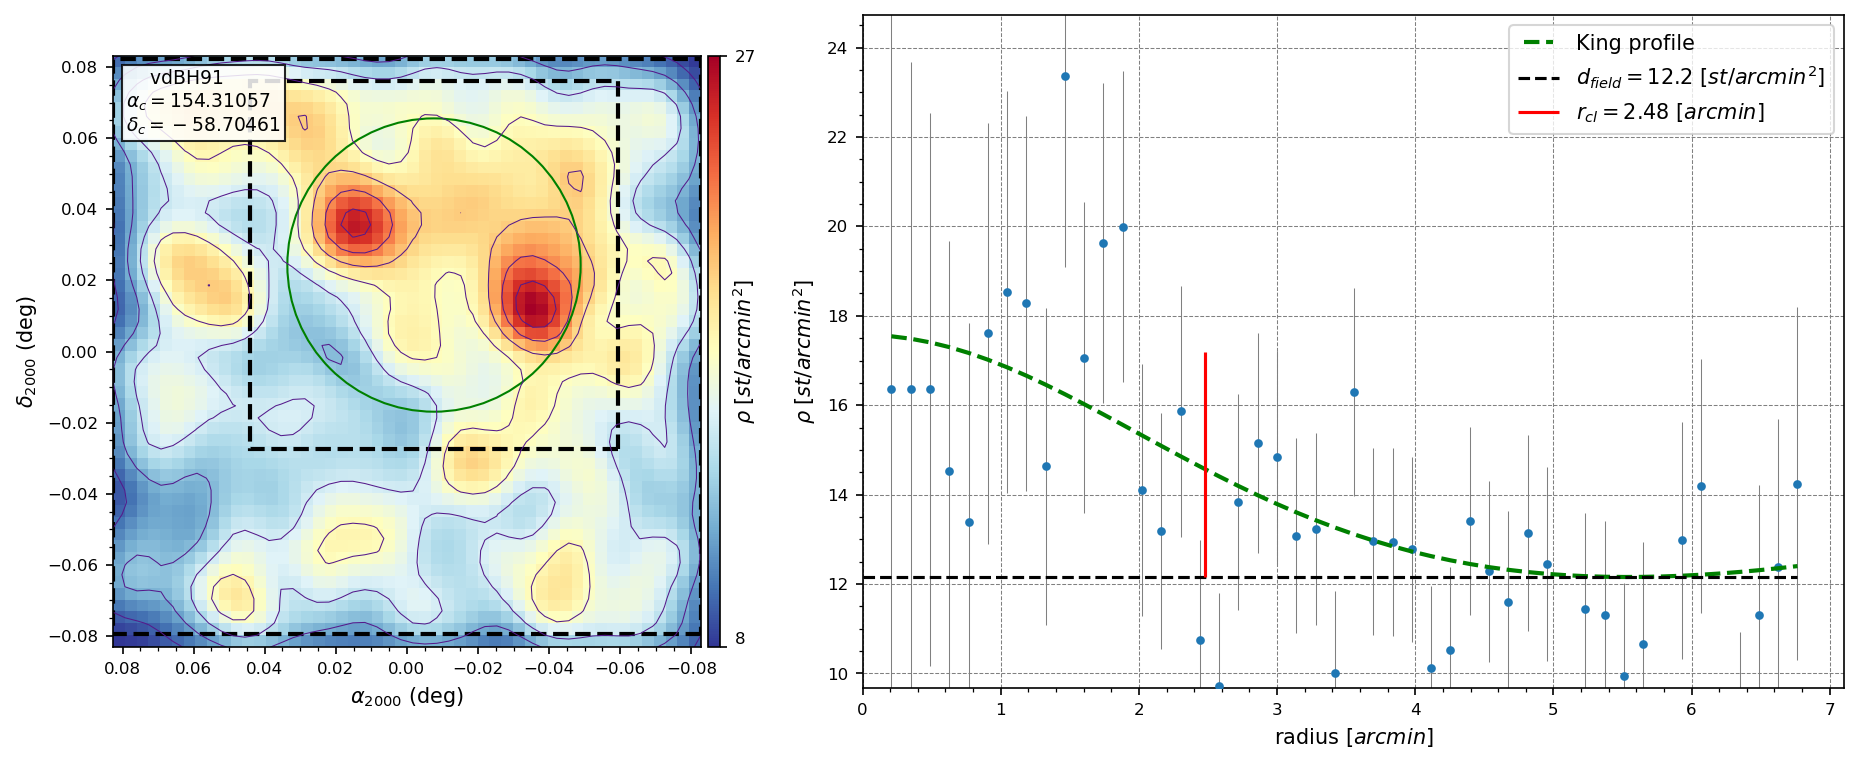
\includegraphics[width=\hsize]{figs/high_res/dmap_vdbh91.png}
    \caption{Idem Fig. \ref{fig4} for vdBH 91.}
    \label{fig28}
\end{figure*}
\begin{figure*}[ht]
    \centering
    \includegraphics[width=\hsize]{figs/high_res/cmds_vdbh91.png}
    \caption{Idem Fig. \ref{fig5} for vdBH 91.}
    \label{fig29}
\end{figure*}
\begin{figure*}[ht]
    \centering
    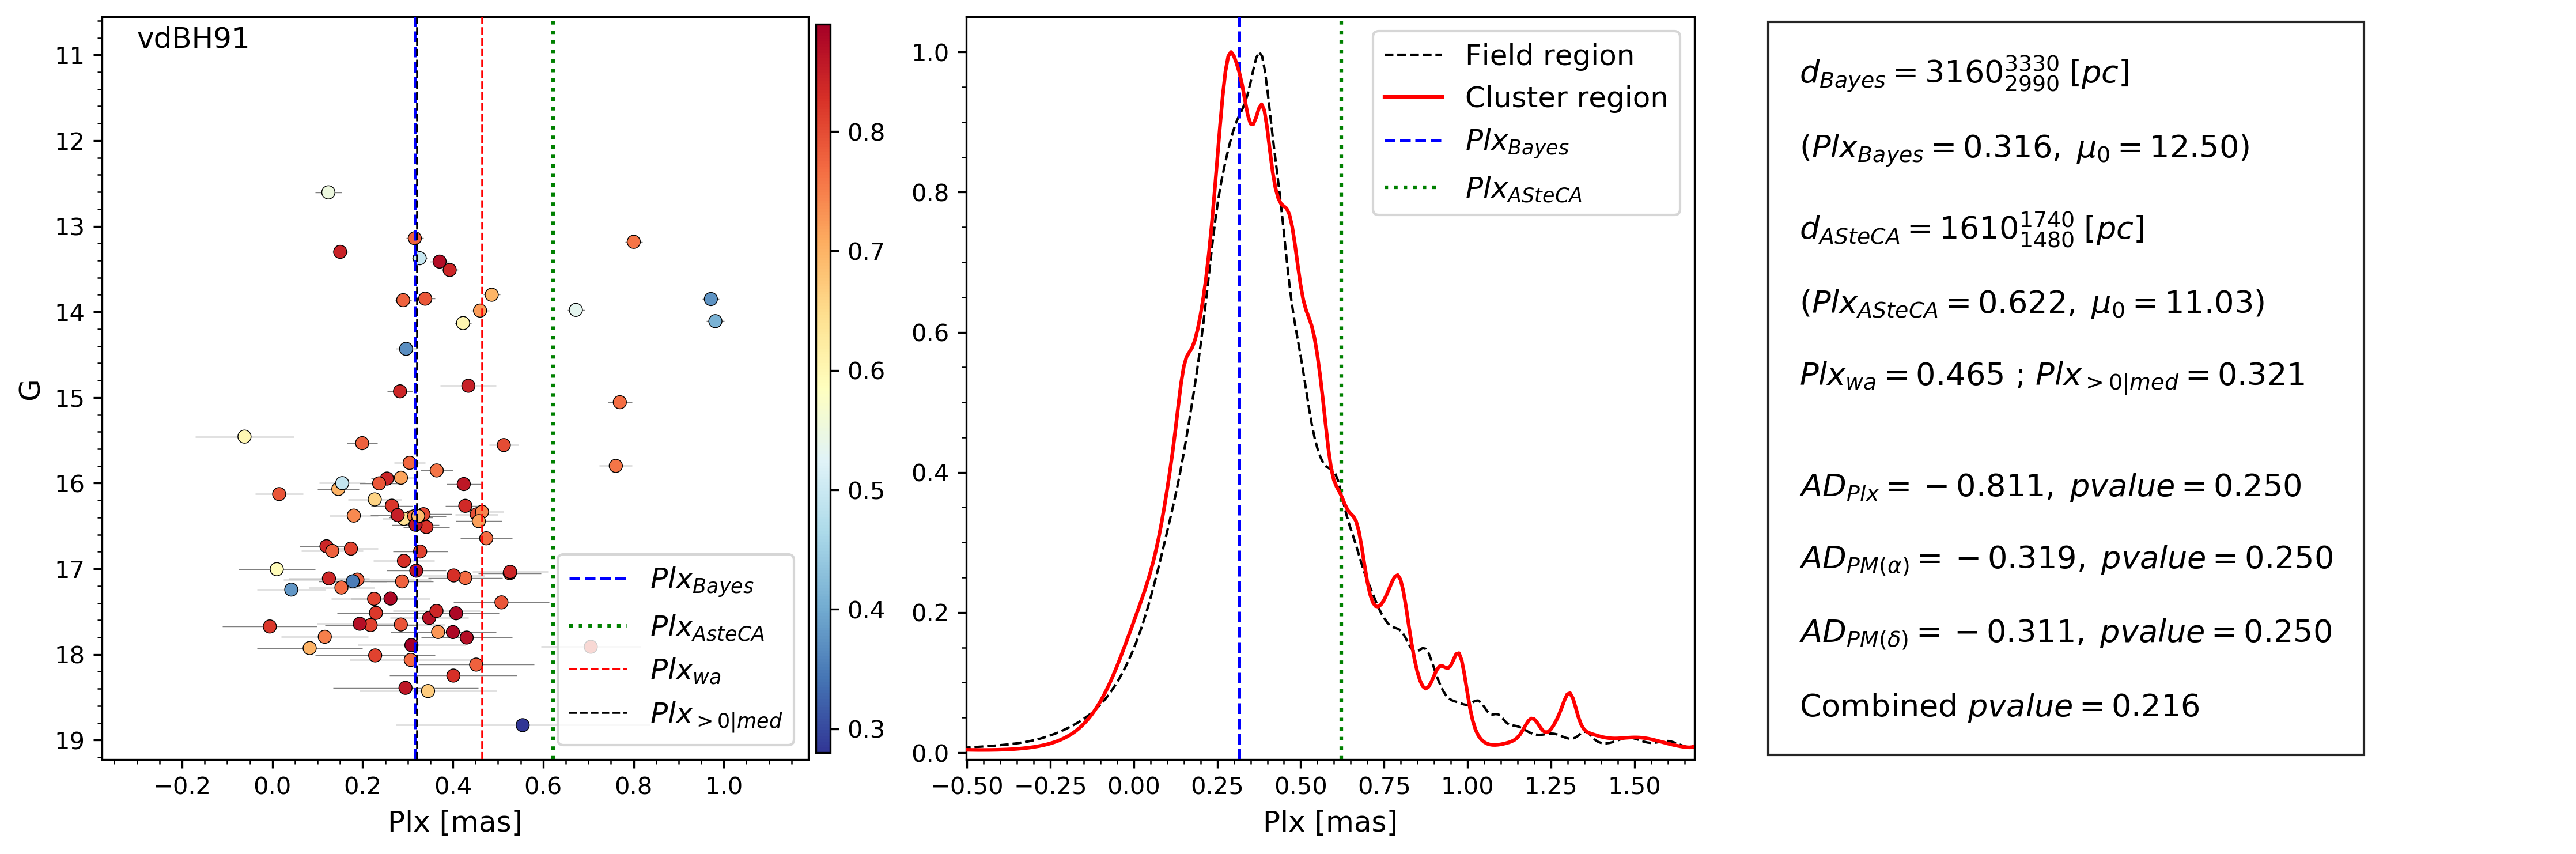
\includegraphics[width=\hsize]{figs/high_res/plx_vdBH91.png}
    \caption{Idem Fig. \ref{fig6} for vdBH 91.}
    \label{fig30}
\end{figure*}



%================================================================
\section{Ruprecht 88}

RUP 88 is another potential cluster south of the Carina HII region. Like
other objects in this paper no obvious stellar grouping is perceived in the $V$
image of Fig. \ref{fig2}. The overall star CMDs in Fig. \ref{fig31} show a
scattered star distribution above $V = 16$ mag. From this magnitude down the
common pattern of galactic disc stars takes place in the CMDs. The CCD in Fig.
\ref{fig31} suggests that no blue and therefore young star is present in the
region of RUP 88. Just at $0.2 < (B-V) < 0.8$ we see a handful of stars that
could be reddened late of late $B$- types or $A-F$-type stars. The remaining of
this diagram is a trace composed by $A$- to $M$-type stars.\\

Like in other clusters in the present sample when the spatial distribution of
stars in the frame is analyzed, it happens that no clear star overdensity
appears in the location where RUP 88 is supposed to exist. In fact, the
contour plot in Fig. \ref{fig32}, left panel, shows a poor star number
enhancement from south west to northeast of the frame extending north west.
Given the difficulties to state the position of the cluster center (if it
exists) we ask \texttt{ASteCA} to inspect the region encircled in green in Fig.
\ref{fig32}, where a reasonable density profile could be found. But anyway the
RDP is still noisy because of a rather poor star number contained between the
assumed cluster limits. If we look at Fig. \ref{fig33}, in the CMDs, only 46
stars with probabilities ranging from 0.24 to 0.57 remain inside the adopted
cluster region, quite low membership probability numbers perhaps reflecting the
trouble to set aside the cluster region from the field region. The findings in
the three photometric diagrams in Fig. \ref{fig33} confirm this point as only an
amorphous distribution of stars scarcely resembling a cluster main sequence can
be seen.\\

The Anderson-Darling test in Fig. \ref{fig34}, right panel, states differences
between cluster and field stars only in the case of the $PM(\alpha)$, while
for the rest of variables, $Plx$ and $PM(\delta)$ the test is unable to separate
the cluster population from the one from the field region. Despite this, the
combined $p$-value for proper motions and parallaxes is low (but still larger
than the critical 5\% value usually employed as a threshold to reject the
null hypothesis)
suggesting that both samples do not come from the same population. However, the
necessary requirement that there is a reasonable main sequence is absent and
therefore precludes concluding that RUP 88 is a true cluster.

\begin{figure*}[ht]
    \centering
    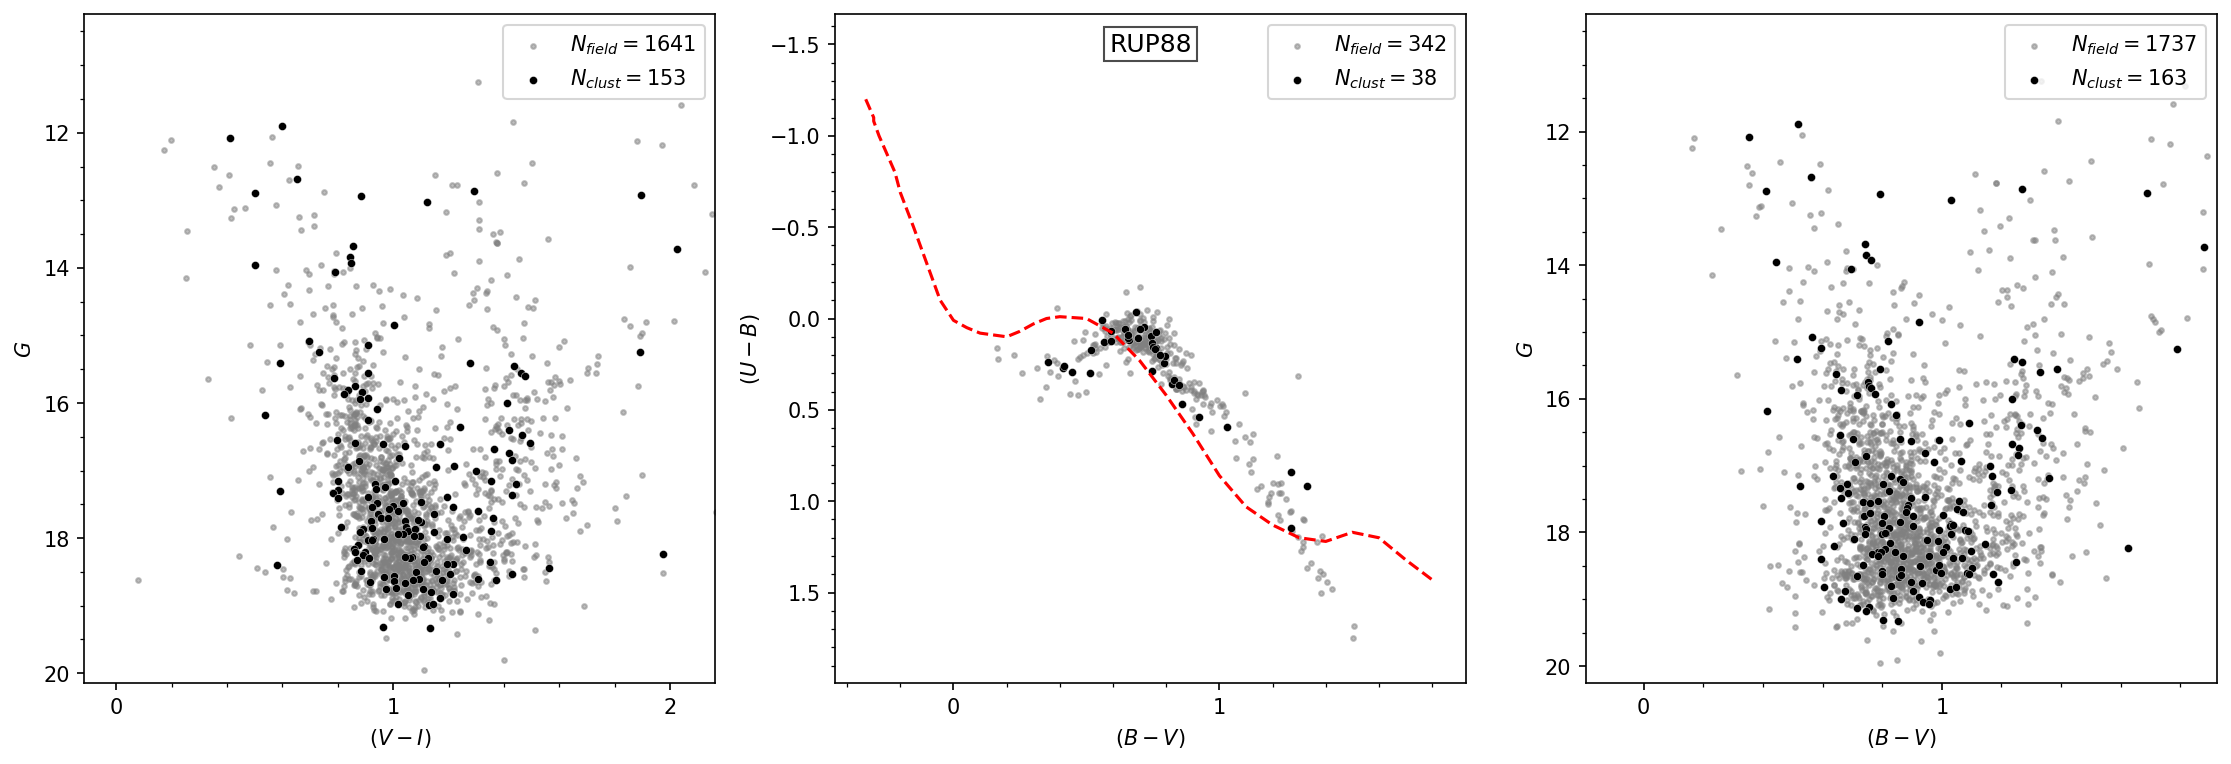
\includegraphics[width=\hsize]{figs/high_res/obs_RUP88.png}
    \caption{Idem Fig. \ref{fig3} for RUP 88.}
    \label{fig31}
\end{figure*}
\begin{figure*}[ht]
    \centering
    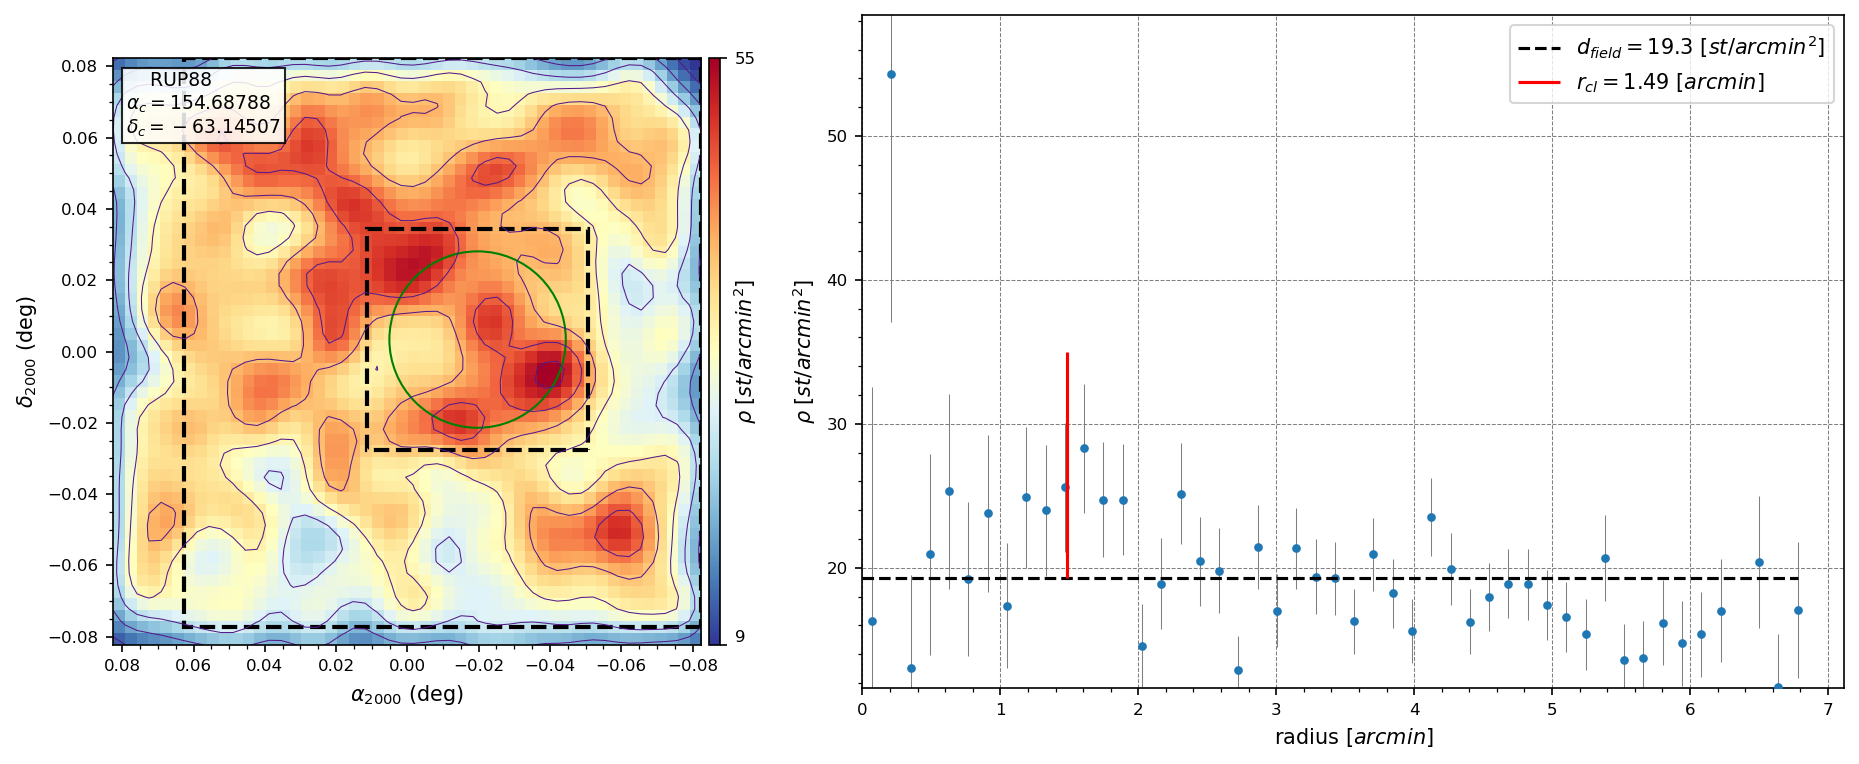
\includegraphics[width=\hsize]{figs/high_res/dmap_rup88.png}
    \caption{Idem Fig. \ref{fig4} for RUP 88.}
    \label{fig32}
\end{figure*}
\begin{figure*}[ht]
    \centering
    \includegraphics[width=\hsize]{figs/high_res/cmds_rup88.png}
    \caption{Idem Fig. \ref{fig5} for RUP 88.}
    \label{fig33}
\end{figure*}
\begin{figure*}[ht]
    \centering
    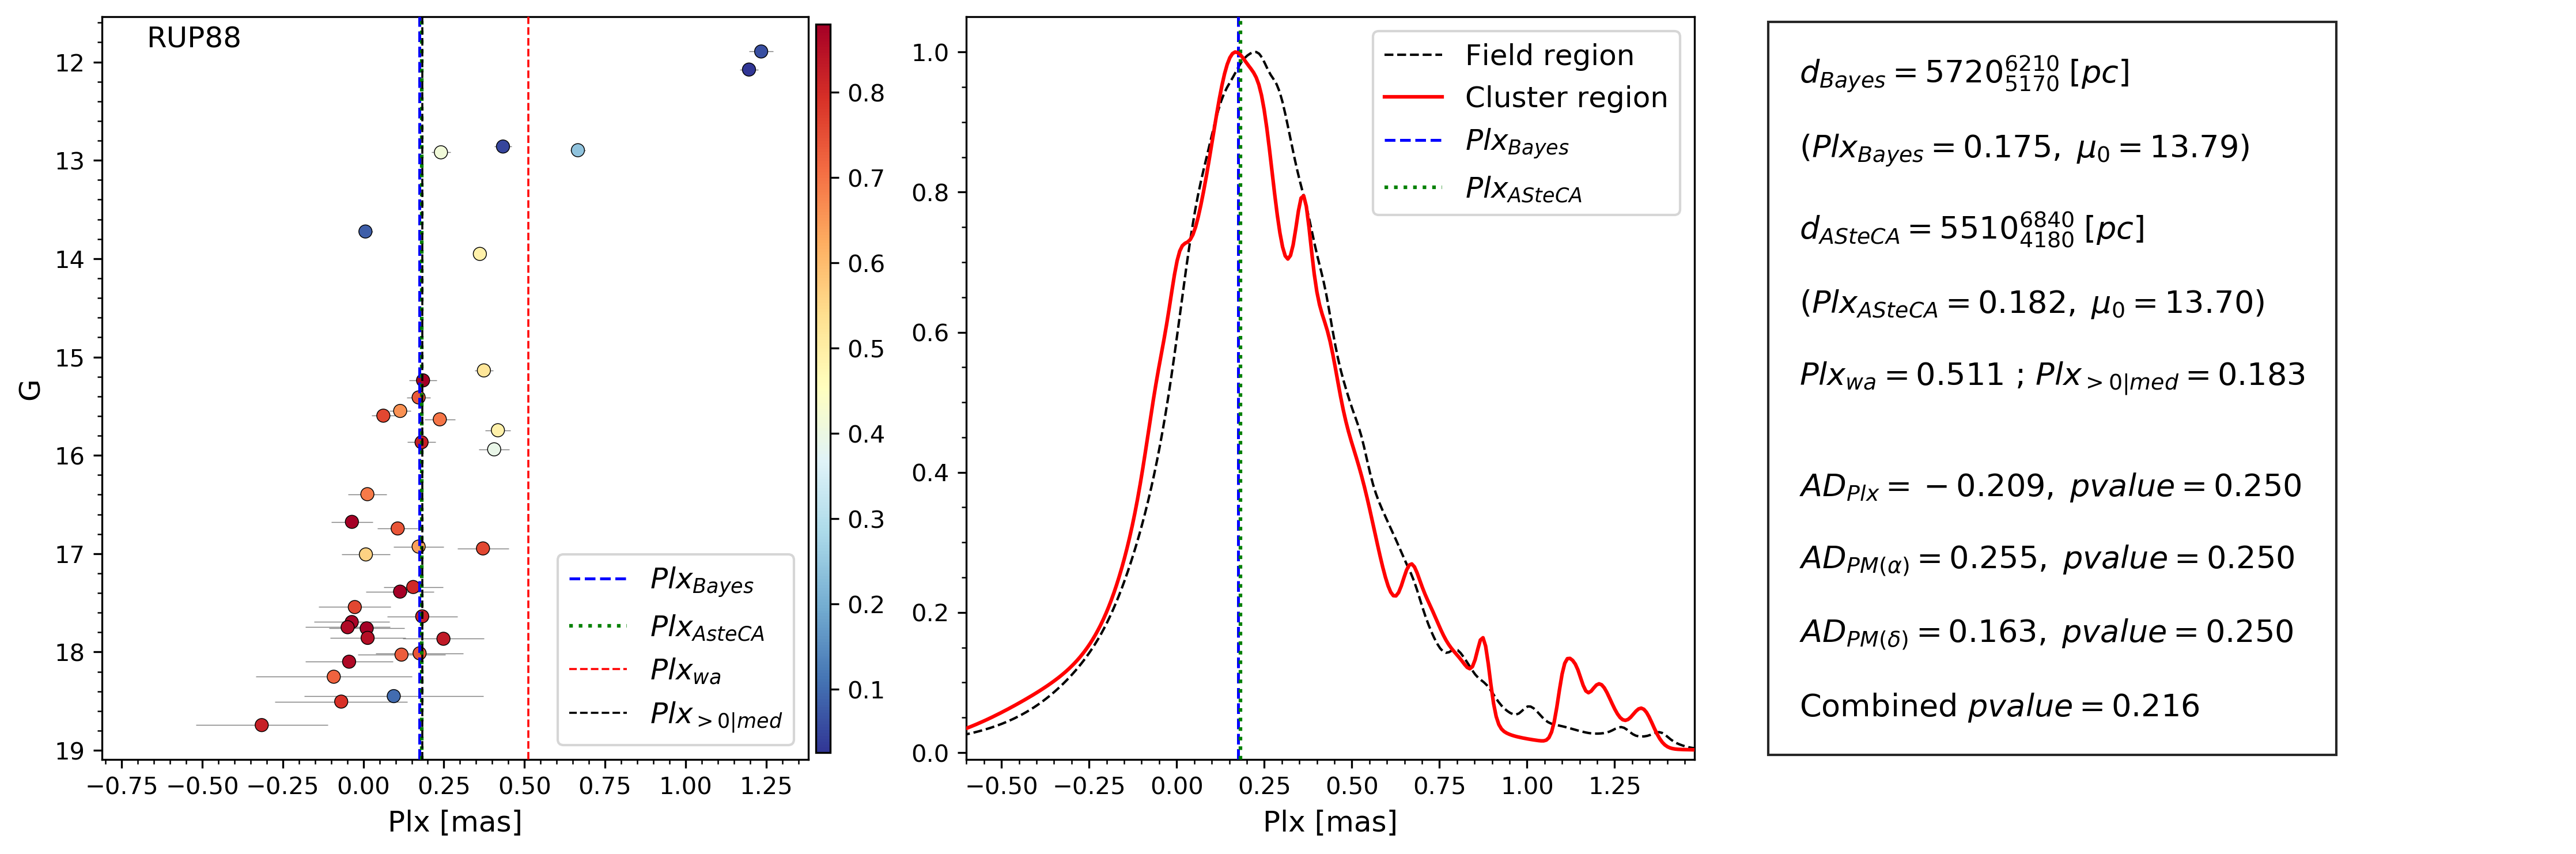
\includegraphics[width=\hsize]{figs/high_res/plx_RUP88.png}
    \caption{Idem Fig. \ref{fig6} for RUP 88.}
    \label{fig34}
\end{figure*}




%================================================================
\section{van den Bergh-Hagen 92}

Placed south of Vela, near the eastern border with Carina, vdBH
92 is a relevant handful of bright stars as seen in the $V$ image of Fig.
\ref{fig2}. The CMDs and CCD for all stars in the region, as shown in Fig.
\ref{fig35}, depict a narrow star sequence with some scatter at their respective
bright ends. Particularly the CCD shows, not far from the intrinsic line, a
group of $F$- and $G$-type stars and another group of stars below the intrinsic
line that could be $B$- and $A$- type stars displaced by the reddening effect.\\

\texttt{ASteCA} analysis in Fig. \ref{fig36} revealed the presence of a well
isolated star overdensity rising above the field stars density of about 4
stars per square arcmin. We identify this overdensity with vdBH
92. Notwithstanding the noisy RDP the limits of the overdensity can be well
established. As indicated in Fig. \ref{fig37} few stars have been found inside
the cluster limits with membership values from 0.65 to 0.95. Despite such a low
number of members, a 7 magnitude extended cluster main sequence has been found
outlined by stars with probabilities above 0.7 approximately. The comparison
with synthetic clusters made by \texttt{ASteCA} yields:

\begin{itemize}
\item [a)] the best fitting of a synthetic cluster to the clean data in Fig. 
    \ref{fig37} indicates a color excess of $E_{(B-V)} = 0.58$. Since the
    maximum color excess provided by S\&F2011 is 2.34 for this zone we
    conclude that most of the absorption is produced behind the position of van
    den Bergh-Hagen 92. This object is therefore placed in front of a strong
    absorption region.
\item [b)] The absorption free distance modulus becomes 11.44 what places van den
    Bergh-Hagen 92 at a distance of $d = 1.941$ kpc.
\end{itemize}

By applying the Anderson-Darling test it is noticed that the parallax
distributions for stars inside and outside the cluster boundaries are not
different from each other as indicated in the right panel of Fig. 
\ref{fig38}. However, proper motions are quite different in both regions. We
associate this last finding with the presence of a well defined overdensity
that, in turn, shows a
reasonable and extended cluster main sequence to conclude that both samples come
from different populations.\\

All this together confirm the true nature of vdBH 92. This is a
young cluster $112\times10^6$ years old.

\begin{figure*}[ht]
    \centering
    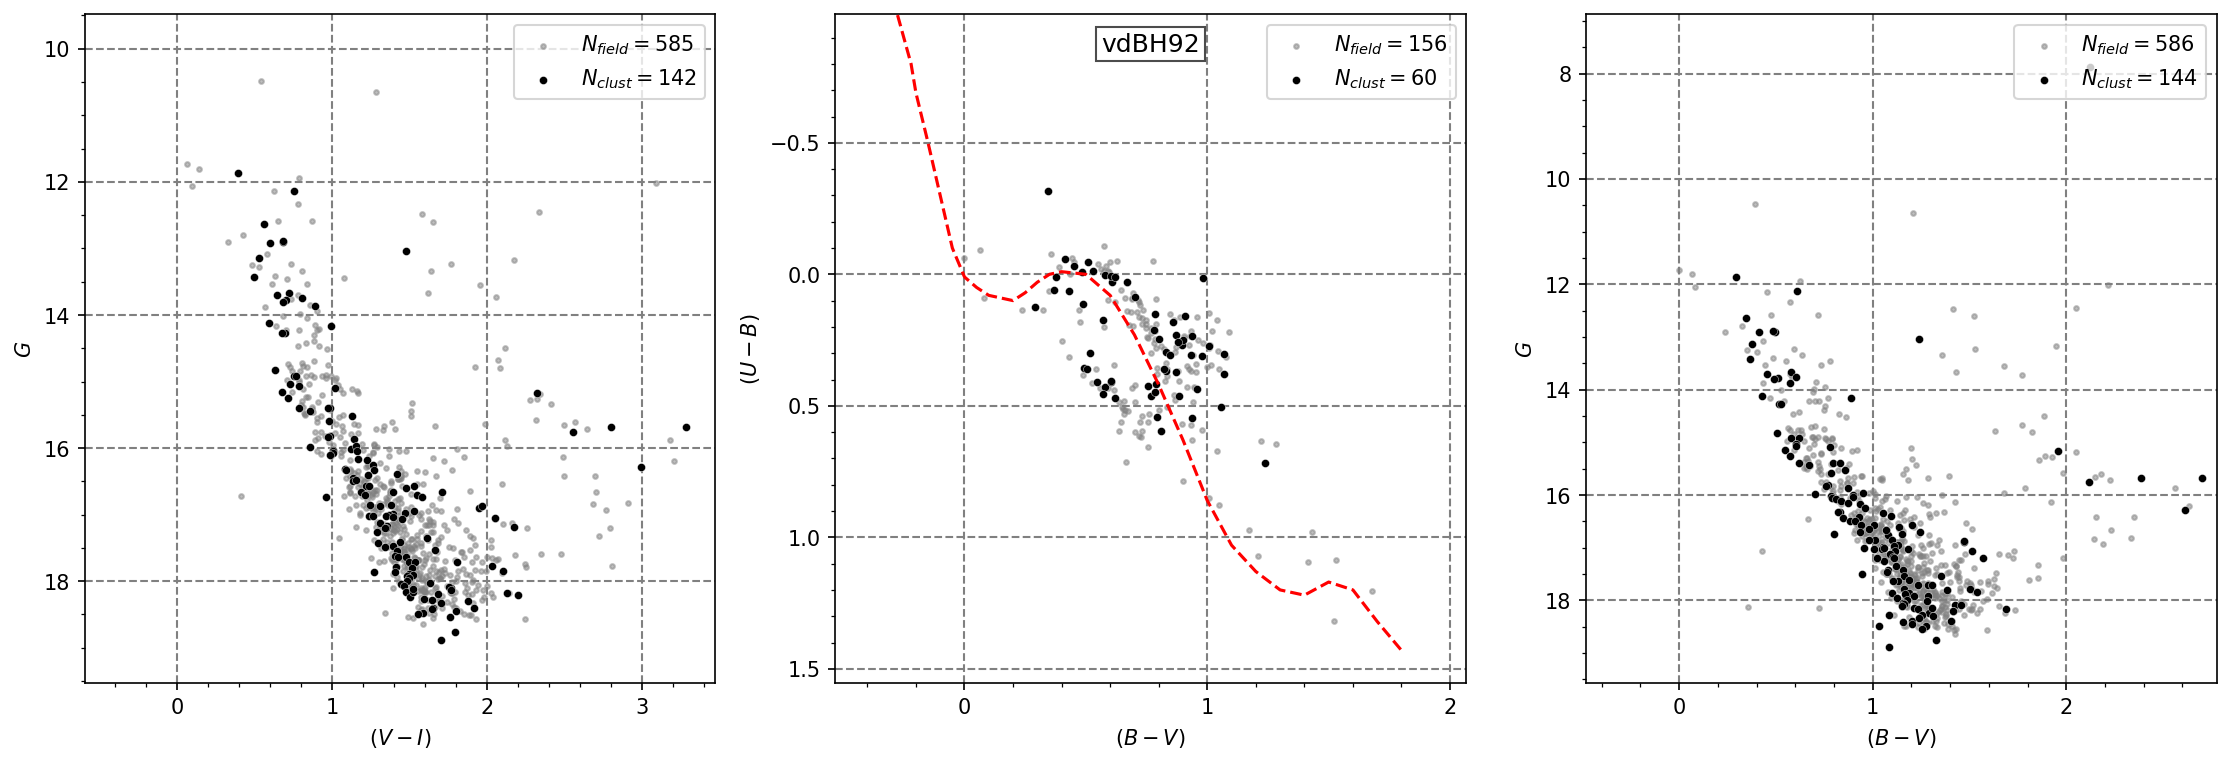
\includegraphics[width=\hsize]{figs/high_res/obs_vdBH92.png}
    \caption{Idem Fig. \ref{fig3} for vdBH 92.}
    \label{fig35}
\end{figure*}
\begin{figure*}[ht]
    \centering
    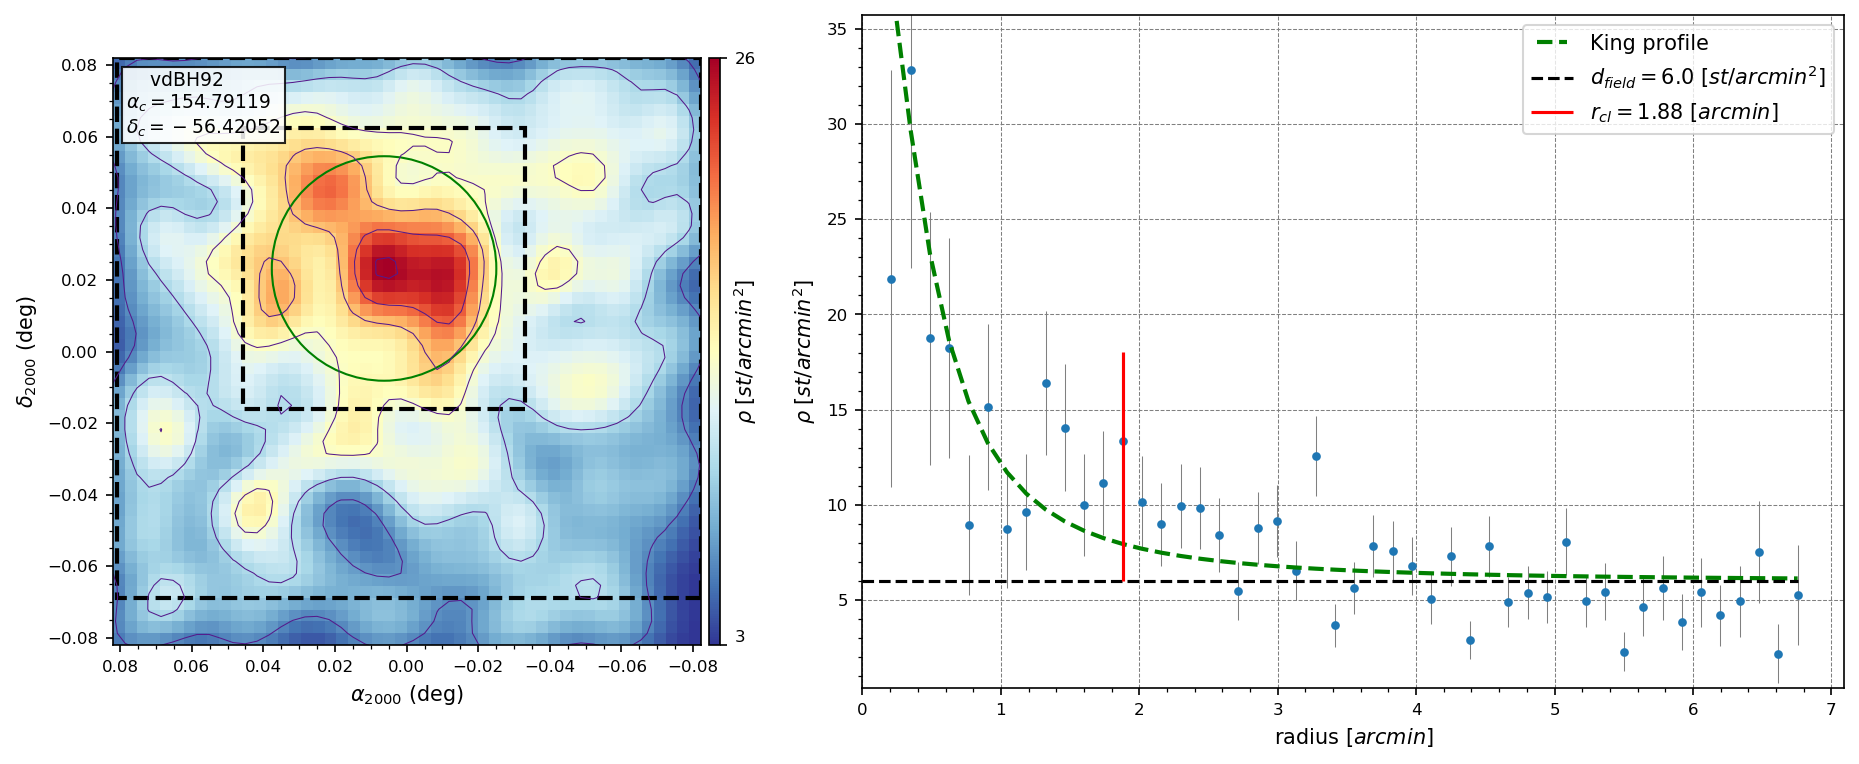
\includegraphics[width=\hsize]{figs/high_res/dmap_vdbh92.png}
    \caption{Idem Fig. \ref{fig4} for vdBH 92.}
    \label{fig36}
\end{figure*}
\begin{figure*}[ht]
    \centering
    \includegraphics[width=\hsize]{figs/high_res/cmds_vdbh92.png}
    \caption{Idem Fig. \ref{fig5} for vdBH 92.}
    \label{fig37}
\end{figure*}
\begin{figure*}[ht]
    \centering
    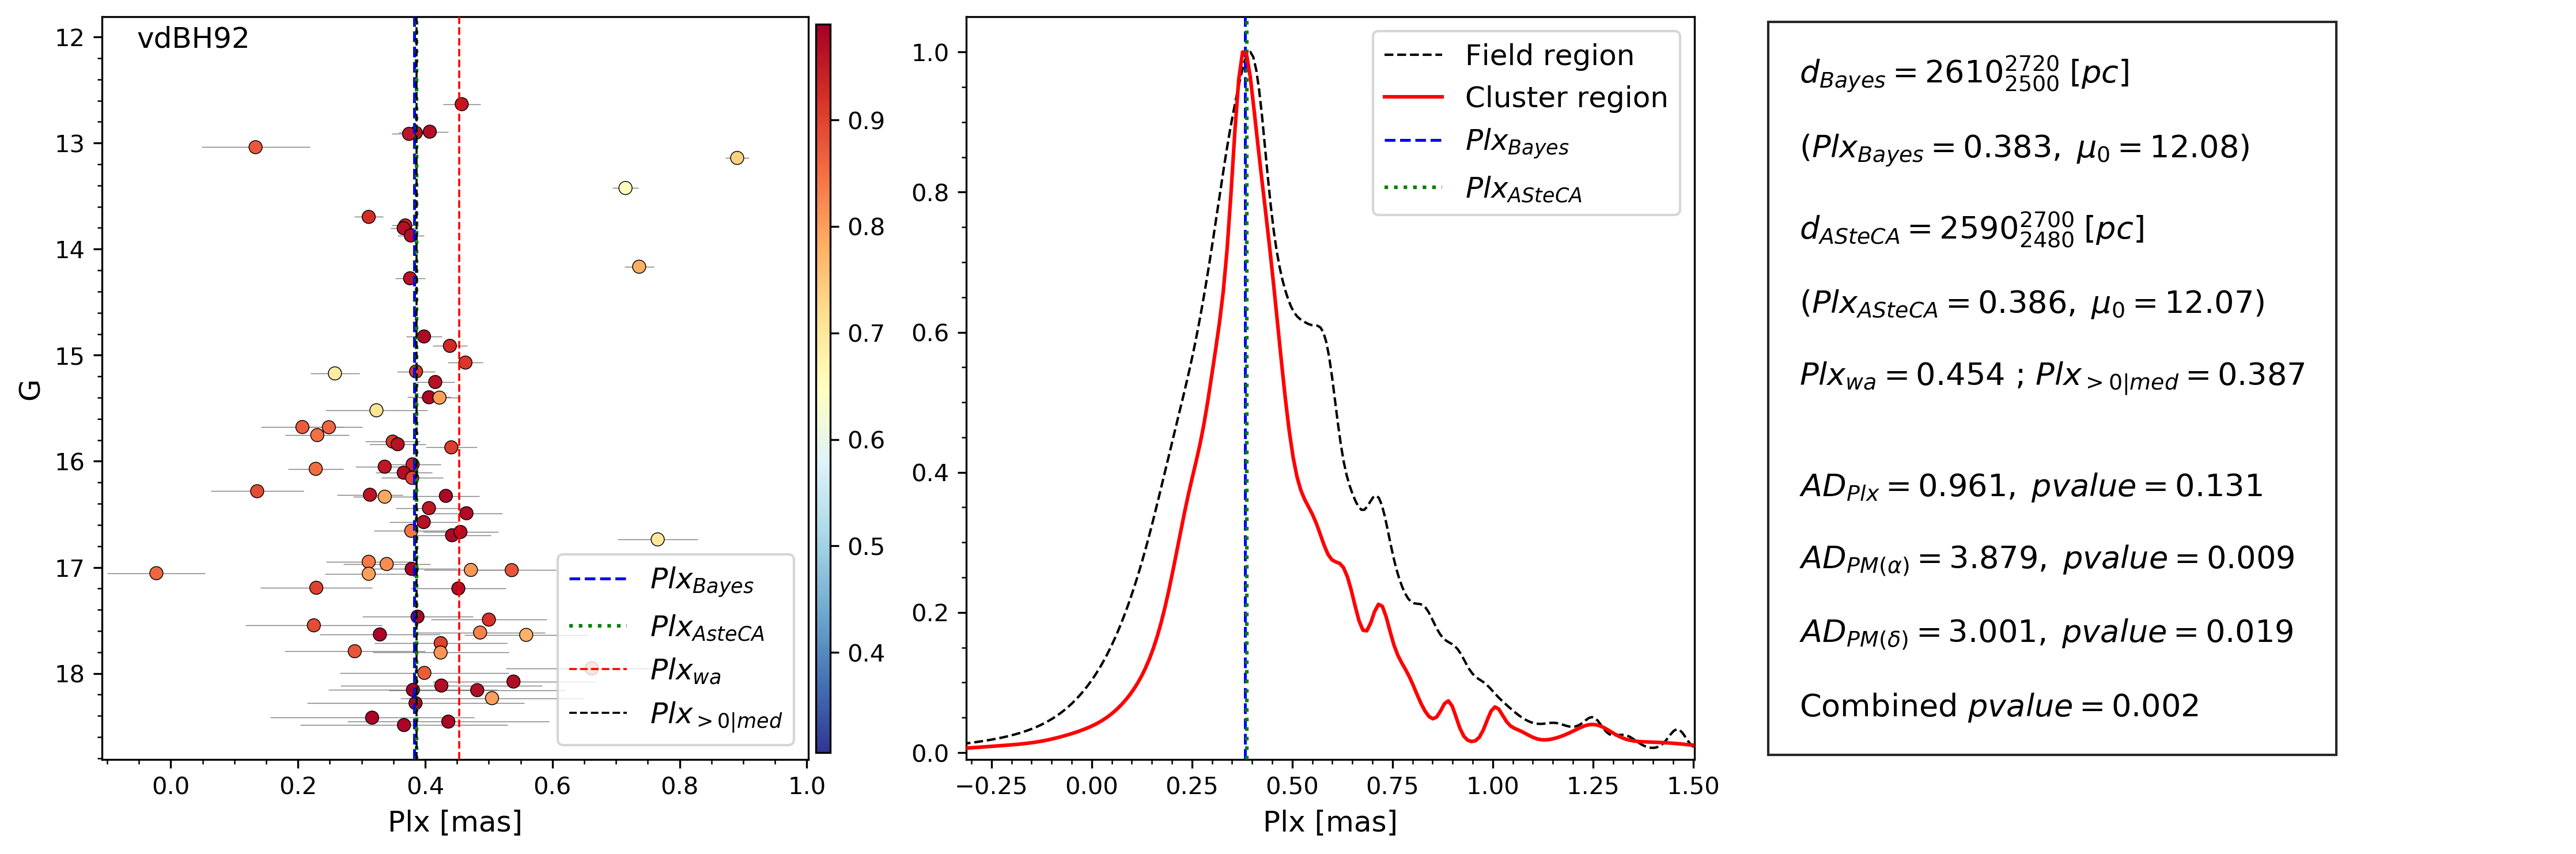
\includegraphics[width=\hsize]{figs/high_res/plx_vdBH92.png}
    \caption{Idem Fig. \ref{fig6} for vdBH 92.}
    \label{fig38}
\end{figure*}



%================================================================
\section{Trumpler 13}

TR 13 is a weak object also at the south west of the Carina HII
region, seen as a diffuse but extended star accumulation near the center of the
$V$ image in Fig. \ref{fig2}. The two CMDs in Fig. \ref{fig39} show an uncommon
pattern: we see that above $V = 17.5$ mag the star sequence splits into two
branches with one of them extending to the bluest side while other branch
follows the common representation of galaxy disc stars.
In the CCD the situation is the same: a
wide and reddened band of potential $B$-type stars is placed for $(B-V)<0.45$
and for $-0.25<(U-B)<0.5$ with a few more stars at negative $(U-B)$ index
while another strip of stars goes from the characteristic place for $F$-type
stars extending to the red tail including probable giant stars.\\

Fig. \ref{fig40} indicates that \texttt{ASteCA} found a spatially extended
overdensity mostly elongated north-south, which, at its peak is nearly 5 times
above a mean field stellar density of 12 stars per square arcmin. Given the
shape and extension of the overdensity we adopted a formal radius 3.7 arcmin and
asked \texttt{ASteCA} to compute the membership probabilities for those stars
inside the area. Fig. \ref{fig41} shows that after the removal of field
interlopers, over 180 stars with membership values from 0.34 to 0.81 are left
composing a narrow cluster main sequence extending for more than 6 magnitudes.
Consequently, when comparing with synthetic clusters the results yield:

\begin{itemize}
\item [a)] A color excess of $E_{(B-V)}= 0.50$ is found for the best fitting of a
    synthetic cluster. Since the maximum color excess provided by S\&F2011
    is 1.94 it is reasonable to conclude that most of the absorption is produced
    behind the position of TR 13.
\item [b)] The absorption free distance modulus of TR 13 becomes 13.25
    placing it at a distance of 4.467 kpc from the Sun.
\end{itemize}

The Anderson-Darling statistics in Fig. \ref{fig42}, right panel, confirm the
photometric results. In fact, cluster area and the surrounding field region
possess quite different properties.\\

Although not particularly large, probabilities for stars inside the
overdensity confirm the true nature of this object since the over density
and the density profile are followed by a very well defined and extended
photometric counterpart. All these facts joined to the results from the
Anderson-Darling test are self-consistent, so that we are confident that
TR 13 is a young cluster $56\times10^6$ years old.

\begin{figure*}[ht]
    \centering
    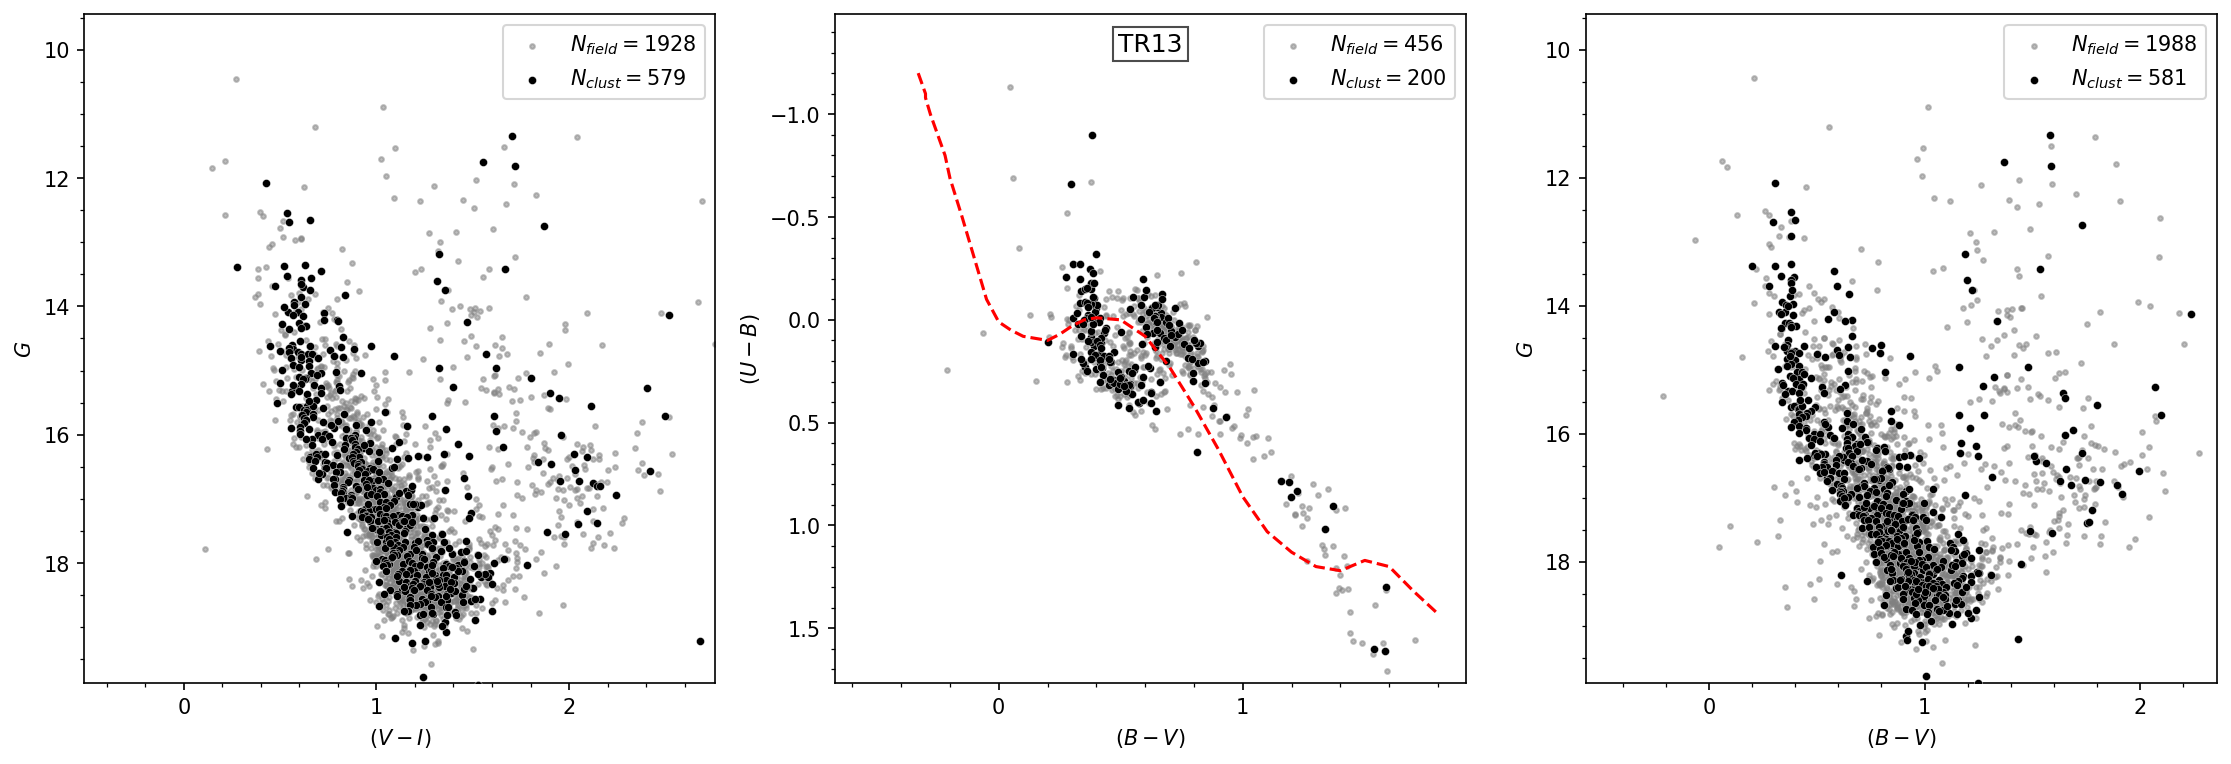
\includegraphics[width=\hsize]{figs/high_res/obs_TR13.png}
    \caption{Idem Fig. \ref{fig3} for TR 13.}
    \label{fig39}
\end{figure*}
\begin{figure*}[ht]
    \centering
    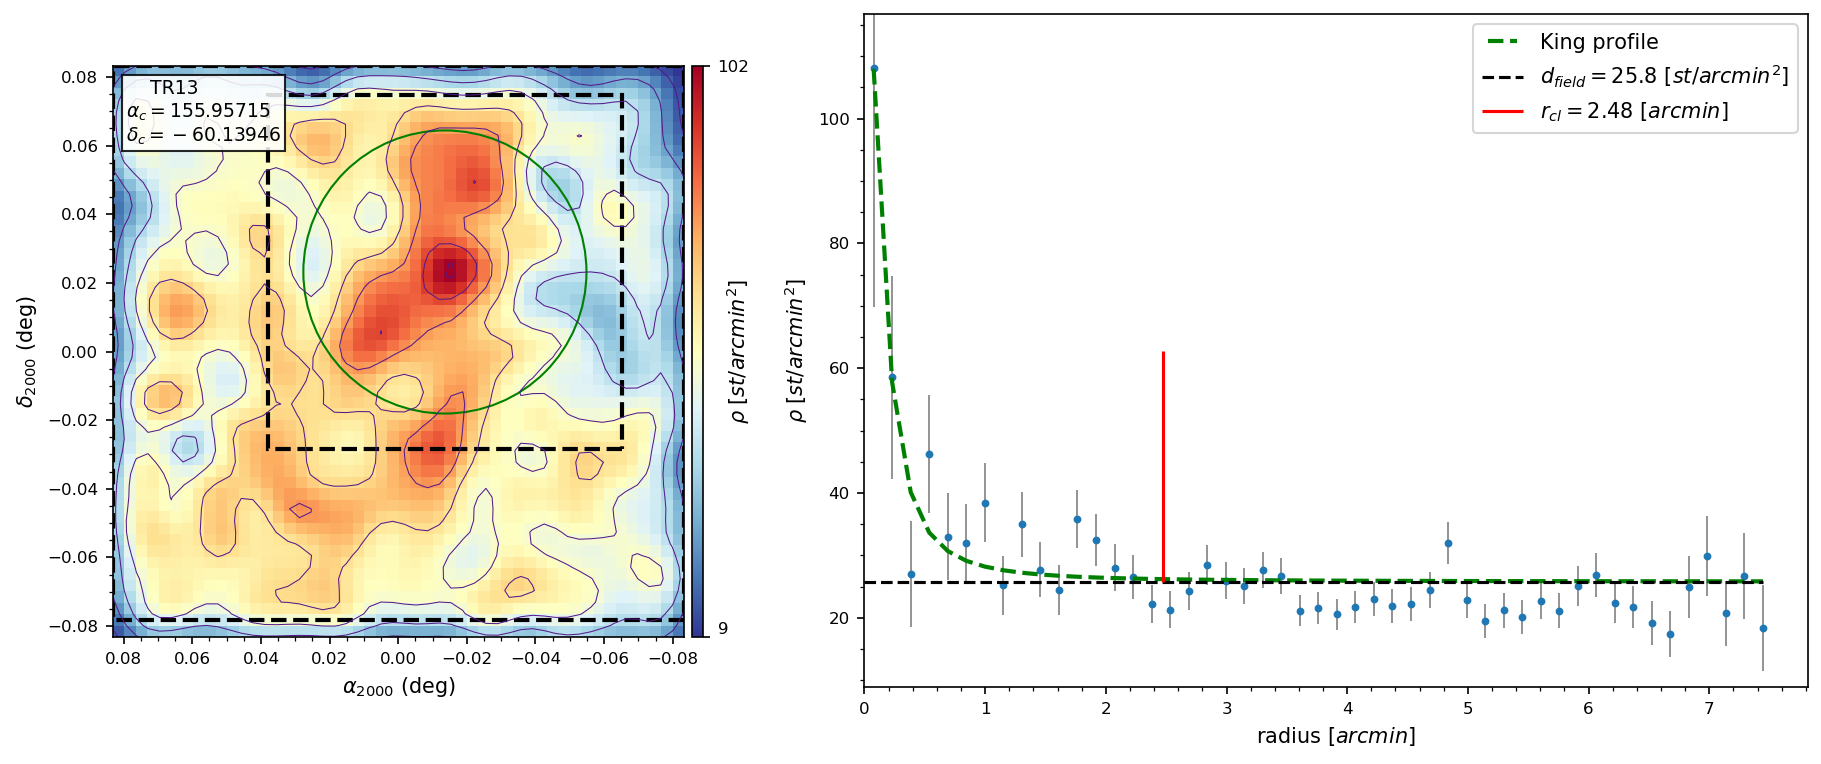
\includegraphics[width=\hsize]{figs/high_res/dmap_trumpler13.png}
    \caption{Idem Fig. \ref{fig4} for TR 13.}
    \label{fig40}
\end{figure*}
\begin{figure*}[ht]
    \centering
    \includegraphics[width=\hsize]{figs/high_res/cmds_tr13.png}
    \caption{Idem Fig. \ref{fig5} for TR 13.}
    \label{fig41}
\end{figure*}
\begin{figure*}[ht]
    \centering
    \includegraphics[width=\hsize]{figs/high_res/plx_TR13.png}
    \caption{Idem Fig. \ref{fig6} for TR 13.}
    \label{fig42}
\end{figure*}



%================================================================
\section{van den Bergh-Hagen 106}

This cluster is placed at the south-east of the Vela constellation. The not so
dense stellar field where it is placed has no relevant features except a few
moderately bright stars as shown in Fig. \ref{fig2}. The CMDs shown in
Fig. \ref{fig43} represent typical photometric features structures of galactic
fields with no cluster inside. As for the CCD in the same figure it shows a
reduced number of stars below the intrinsic line (probably reddened late $B$-
and $A$ types) and a tail of stars from of late $F$-types to $M$-type stars
–some of them probably giant- at the red end.
\texttt{ASteCA} spatial analysis found some star clumps as seen in Fig. 
\ref{fig44}, left panel. We focus the attention on the main one at the very
center of the frame, since here we see the highest overdensity peak with 4 times
more stars than at the mean stellar background density of 7 stars per square
arcmin approximately. We assume that most of stars in vdBH 106
must be included there so the cluster parameters should be well established. It
is a fact that the RDP appears not well defined since it reflects the irregular
and poor star density even inside the zone selected to investigate the cluster
parameters. Only 79 stars have been found inside this area. Indeed the
membership values for stars inside the putative cluster position range from 0.31
to 0.69. However, those stars having probabilities near the maximum values in
this region still outline a cluster main sequence that can be fitted with a
synthetic cluster which yields the following parameters:

\begin{itemize}
\item [a)] A color excess of $E_{(B-V)} = 0.33$ has been found to affect the
    cluster. This value is well in line with the maximum color excess provided
    by S\&F2011, $E_{(B-V)} = 0.57$ in this direction.
\item [b)] The absorption free distance modulus of vdBH 106 was
    found to be 13.22 what puts the cluster at a distance of $d=4.406$ kpc from
    the Sun.
\end{itemize}

In this region we found from the application of the Anderson-Darling test that
the parallax and proper motion distributions seem to belong to the same
originating distribution, as seen in Fig. \ref{fig46}. Indeed, the moderately
high combined p-value makes the rejection of the null hypothesis difficult,
since the probability of erroneously rejecting it is around $22\%$.\\

Despite a trace of a sequence belonging to a typical old cluster is
noticeable in Fig. \ref{fig45}, we are cautious as to confirm its nature.
Clearly deeper photometric observations (particularly in the $U$ filter) are
needed. Meanwhile and under the assumption we are facing a true object van
den Bergh-Hagen 106 could be an open cluster around $1122\times10^6$ years
old.

\begin{figure*}[ht]
    \centering
    \includegraphics[width=\hsize]{figs/high_res/obs_vdBH106.png}
    \caption{Idem Fig. \ref{fig3} for vdBH 106.}
    \label{fig43}
\end{figure*}
\begin{figure*}[ht]
    \centering
    \includegraphics[width=\hsize]{figs/high_res/dmap_vdbh106.png}
    \caption{Idem Fig. \ref{fig4} for vdBH 106.}
    \label{fig44}
\end{figure*}
\begin{figure*}[ht]
    \centering
    \includegraphics[width=\hsize]{figs/high_res/cmds_vdbh106.png}
    \caption{Idem Fig. \ref{fig5} for vdBH 106.}
    \label{fig45}
\end{figure*}
\begin{figure*}[ht]
    \centering
    \includegraphics[width=\hsize]{figs/high_res/plx_vdBH106.png}
    \caption{Idem Fig. \ref{fig6} for vdBH 106.}
    \label{fig46}
\end{figure*}



%================================================================
\section{Ruprecht 162}
\label{app:rup162}

Placed to the south east of the Carina HII region, the $V$ image of the region
in Fig. \ref{fig2} where the cluster is supposed to exist shows a moderate
number of stars resembling a star grouping placed at the north-west in the
frame. At first sight the CMDs in Fig. \ref{fig47} for the overall stars look
as if a cluster main sequence is emerging from the trace of the disk star
distribution.
In the same figure, right panel, the CCD splits into two star groups: one of
them is mostly placed below the intrinsic line for $0.0<(B-V)< 0.8$ and
resembles a strip of reddened blue stars (including early and late $B$-types
and, perhaps, some $A$-type stars); the other group shows a distribution of $F$-
to $M$-type stars strongly affected by reddening in appearance.\\

\texttt{ASteCA} detected an extended and irregular region at the north-west of
the frame in Fig. \ref{fig48} (where the cluster is supposed to lie). Given the
difficulties to set a clear overdensity we decided to focus the attention on the
zone encircled in green in Fig. \ref{fig48}, left panel. The background mean star
density is over 12 stars per squared arcmin and, at the most, the overdensity is
just 20 stars at the maximum. This produces unavoidably a noisy RDP (it is hard
to establish a meaningful radius and there is a quite irregular star
distribution across the zone).
The CMDs and CCD in Fig. \ref{fig49} after the removal of field interlopers tell
us that stars in the adopted cluster region have membership probabilities in the
range 0.32 to 0.93. Stars above $V=16$ mag have membership values over 0.6 but
are all scattered in the range $0.2<(B-V)<2.6$. When one looks closely at the
right and left panels in Fig. \ref{fig49}, a small group of stars with the
largest memberships appear following something like a cluster main sequence.
The cleaned CCD, Fig. \ref{fig49} mid panel, leaves a blue sequence of stars
suffering some internal color scatter followed by a tail of $F$- to $K$-type
stars. Therefore this object could be more extended than supposed. 
\texttt{ASteCA} found the best fitting with a synthetic cluster with the
following properties:

% TODO arreglar intervalo
\begin{itemize}
\item [a)] The color excess affecting the cluster is $E_{(B-V)} = 0.25$ inside
    the values given by S\&F2011 who estimate $E_{(B-V)} = 1.07$ at
    maximum and 0.91 at minimum. 
\item [b)] The absorption free distance modulus is 11.90 corresponding to a
    distance of $d = 2.399$ kpc.
\end{itemize}

Proper motions $PM(\alpha)$ and $PM(\delta)$ in the location of RUP 162 and
the surrounding field region are not different enough from each other as to be
efficiently disentangled. However, the $Plx$ for cluster and field stars are
well differentiated according to the statistical test results shown in Fig.
\ref{fig50}, right panel.\\

Although weak enough the presence of a probable main sequence in the 
panels of Fig. \ref{fig49} and the fact that the Anderson-Darling test
yields that the $Plx$ distributions are different, make us cautious
leaving some chance for RUP 162 to be a true and young cluster about
$14\times10^6$ yr old. An additional reinforcement as for the hypothetical
true entity of this young object is the existence of a sudden gap along the
main sequence at $V = 16-16.5$ mag and the presence of high probability
stars at the red side resembling traces of a pre-main sequence. Certainly we
are just speculating on this fact so that more and deeper observations are
needed to arrive to a concluding result for RUP 162.

\begin{figure*}[ht]
    \centering
    \includegraphics[width=\hsize]{figs/high_res/obs_RUP162.png}
    \caption{Idem Fig. \ref{fig3} for RUP 162.}
    \label{fig47}
\end{figure*}
\begin{figure*}[ht]
    \centering
    \includegraphics[width=\hsize]{figs/high_res/dmap_rup162.png}
    \caption{Idem Fig. \ref{fig4} for RUP 162.}
    \label{fig48}
\end{figure*}
\begin{figure*}[ht]
    \centering
    \includegraphics[width=\hsize]{figs/high_res/cmds_rup162.png}
    \caption{Idem Fig. \ref{fig5} for RUP 162.}
    \label{fig49}
\end{figure*}
\begin{figure*}[ht]
    \centering
    \includegraphics[width=\hsize]{figs/high_res/plx_RUP162.png}
    \caption{Idem Fig. \ref{fig6} for RUP 162.}
    \label{fig50}
\end{figure*}




%================================================================
\section{Lynga 15}

% TODO reference?
This is an intriguing object placed in Centaurus, south west between Crux and the
east border of Carina. More specifically, Lynga 15 is about $1^\circ$ north-east
of the star formation region SFR293.64-1.41 \citep{Avedisova_2002}. Like in many
other cases already shown in the $V$ images in Fig. \ref{fig2} this region does
not show, at first glance, any prominent stellar feature though some stars are
bright enough as to attract attention to this place. Maybe the detection of a
planetary nebula (\textcolor{red}{PN Hf 69, reference!}) is another reason to
draw the attention. However, the overall CMDs and CCD shown in Fig. \ref{fig51}
are quite surprising since both CMDs depict an extended sequence (from $V = 8$
down to $V = 16$ mag) emerging toward the left side of the main disc population
trace. In the same figure, right panel, the CCD shows a strip of blue stars
($0.6<(B-V)<0.0$) accompanied by other, probable reddened early type stars,
placed above $(U-B) = 0.0$. The picture seen in the three panels of Fig.
\ref{fig51} induces to think of Lynga 15 as a quite young open cluster.\\

In turn, \texttt{ASteCA} analysis of the spatial structure found an extended and
irregular star overdensity reaching few more than 20 stars per square arcmin.
After many attempts to look for the place where the star membership
probabilities reach the highest values we adopted a 4.6 arcmin radius and set
the potential cluster center in the literature coordinates as indicated in Fig.
\ref{fig52}, left panel. In this place, the RDP displays a 10 stars per squared
arcmin peak above the stellar field density, as seen in the right panel of Fig. 
\ref{fig52}. However, even in this position \texttt{ASteCA} yields a
conflictive result since star membership
probabilities go from 0.34 to 0.96 but as seen in Fig. \ref{fig53}, left and
right panels, a probable cluster main sequence mostly composed by low
probability stars appears below approximately $V = 17$ mag. Above this visual
magnitude the main sequence vanishes and just a handful of stars with the
largest probability values, widely scattered in color index and magnitudes,
takes place. This is, no upper cluster main sequence is evident in the clean
CMDs. It draws the attention that the CCD in the mid panel of Fig. \ref{fig53}
contains a few blue stars with no counterpart in the CMDs. This could be
explained this way: all across the surveyed region there are blue stars (see the
overall CCD in Fig. \ref{fig51}) composing a sort of Blue Plume in the
respective CMDs and just by chance some blue stars also appear in the potential
cluster region after \texttt{ASteCA} analysis (mid panel Fig. \ref{fig53}) but
with low membership probabilities. It could be possible yet that Lynga 15 is an
extended open cluster (even larger than the size of our frame) but the presence
of the huge star gap above $V=17$ mag is unexplainable in a CMD from a
statistical point of view. In our opinion and from a photometric and spatial
point of view Lynga 15 is not an open cluster. The application of the Anderson-
Darling test inform us that the properties of stars inside the adopted cluster
radius and outside of it are almost the same, suggesting no differences between
the two regions.\\

We conclude that Lynga 15 is not a true cluster but a superposition of blue
stars at several distances along the line of sight (see that this is highly
probable). This is not odd at all since this object is not
far from the galactic equator and it is close enough to SFR293.64-1.41 as
indicated above; so, it is probable that blue stars are seen along the direction
to this potential cluster.

\begin{figure*}[ht]
    \centering
    \includegraphics[width=\hsize]{figs/high_res/obs_LYNGA15.png}
    \caption{Idem Fig. \ref{fig3} for Lynga 15.}
    \label{fig51}
\end{figure*}
\begin{figure*}[ht]
    \centering
    \includegraphics[width=\hsize]{figs/high_res/dmap_lynga15.png}
    \caption{Idem Fig. \ref{fig4} for Lynga 15.}
    \label{fig52}
\end{figure*}
\begin{figure*}[ht]
    \centering
    \includegraphics[width=\hsize]{figs/high_res/cmds_lynga15.png}
    \caption{Idem Fig. \ref{fig5} for Lynga 15.}
    \label{fig53}
\end{figure*}
\begin{figure*}[ht]
    \centering
    \includegraphics[width=\hsize]{figs/high_res/plx_LYNGA15.png}
    \caption{Idem Fig. \ref{fig6} for Lynga 15.}
    \label{fig54}
\end{figure*}



%================================================================
\section{Loden 565}

Placed toward the west side of the Crux constellation the $V$ image in Fig. 
\ref{fig2} of Loden 565 does not show any evident star grouping. Inspection of
the CCD and CMDs in Fig. \ref{fig55} only suggests the presence of a dispersed
star group down to $V= 15-16$ mag approximately. From this magnitude down the
overall CMDs show the common pattern of galactic disc star population and
nothing relevant can be seen in the CCD in the mid panel of Fig. \ref{fig55}, but
a modest handful of probable slightly reddened late blue stars for
$(B-V)<0.6$.\\

\texttt{ASteCA} found an irregular overdensity at the north-west corner of the
frame as seen in Fig. \ref{fig56}, left panel. This is the only region across the
entire field where a sudden increase in the star number per area unit is
noticeable showing a 25 stars per squared arcmin peak at its maximum in Fig. 
\ref{fig56}, right panel.
When looking for membership probabilities only a small number of 60 stars remain
inside the adopted radius with probabilities ranging from 0.43 to 0.69, quite
low indeed. Still at such low values a weak lower main sequence appears in the
CMDs in Fig. \ref{fig57} while other stars, above $V = 16$ mag, with larger
values are scattered along the giant branch. Notice that none of the stars that
occupy the CCD of Fig. \ref{fig55} (right panel) with $0<(B-V)<0.6$, with some
chances to be reddened early type stars, remain inside the adopted area after 
\texttt{ASteCA}'s membership analysis. The stars that \texttt{ASteCA}
identified inside the adopted radius could be members of an old group but we
conclude that the photometric evidences are not conclusive at all. More extended
and deeper observations are necessary. Previous estimates of the cluster
parameters found for Loden 565 can be found in \cite{Kharchenko_2005}.
These authors concluded that Loden 565 is a moderately young cluster placed at a
distance of $d = 0.650$ kpc, affected by a mean reddening $E_{(B-V)}= 0.2$ and
a little older than $10^8$ yrs. The \cite{Kharchenko_2005} atlas shows a
poor fitting to a very sparse available data. In addition, when inspecting the
results from the Anderson-Darling test in the right panel of Fig. \ref{fig58}, it
becomes evident that the cluster region is indistinguishable from the stellar
background in term of parallax and proper motion distributions exactly as the
clean CCD and CMDs show in Fig. \ref{fig57}.\\

In conclusion, Loden 565 is more probably a stellar fluctuation.

\begin{figure*}[ht]
    \centering
    \includegraphics[width=\hsize]{figs/high_res/obs_LODEN565.png}
    \caption{Idem Fig. \ref{fig3} for Loden 565.}
    \label{fig55}
\end{figure*}
\begin{figure*}[ht]
    \centering
    \includegraphics[width=\hsize]{figs/high_res/dmap_loden565.png}
    \caption{Idem Fig. \ref{fig4} for Loden 565.}
    \label{fig56}
\end{figure*}
\begin{figure*}[ht]
    \centering
    \includegraphics[width=\hsize]{figs/high_res/cmds_loden565.png}
    \caption{Idem Fig. \ref{fig5} for Loden 565.}
    \label{fig57}
\end{figure*}
\begin{figure*}[ht]
    \centering
    \includegraphics[width=\hsize]{figs/high_res/plx_LODEN565.png}
    \caption{Idem Fig. \ref{fig6} for Loden 565.}
    \label{fig58}
\end{figure*}



%================================================================
\section{NGC 4230}

This object belongs to the Centaurus region immediately close to the upper
border of Crux. The $V$ image in Fig. \ref{fig2} shows that we are facing just a
modest star grouping near the high proper motion star HD 106826
(\textcolor{red}{is this of some value?}) with 8.8 mag. Nothing relevant is
appreciable in the $V$ image of the inspected zone except the star already
mentioned. A highly scattered and diffuse star distribution resembling a boring
galactic disc stellar pattern appears in the overall CCD and CMDs in the panels
of Fig. \ref{fig59}.\\

The spatial inspection performed by \texttt{ASteCA} detected a group of small
stellar overdensities surrounding the central prominence as shown in Fig.
\ref{fig60}, left panel. The peak of the central overdensity shows that the
number of stars per area unit is three times the mean of the background, and the
respective RDP in the right panel of Fig. \ref{fig60} suggests a 2.7 arcmin
radius. However, \texttt{ASteCA} yielded a frustrating result in terms of what
it is expected for a real cluster when analyzing the stellar properties inside
and outside the overdensity. In fact, only 43 stars remain inside the limits we
adopted for NGC 4230 whose membership probability values range from 0.22 to
0.64. At this membership level there is no way to confidently separate the
stellar population into those objects belonging to a real open cluster and those
others belonging to the stellar field. The CCD and CMDs of these 43 stars
in Fig. \ref{fig61} reflect the physical situation since no main sequence is
evident at all. At most, there is a sort of badly defined giant star sequence
whose meaning is dubious because there is no trace of a main sequence. The
comparison with synthetic clusters performed by \texttt{ASteCA} fitted mainly
a group of stars with low brightness, as shown in the CMDs of Fig. \ref{fig61}.
Therefore and accordingly to our analysis there is no cluster called NGC 4230.\\

Results for the distribution of parallax values and proper motions for the
cluster and field regions are yielded in Fig. \ref{fig62}, right panel.
We see that the Anderson-Darling statistics reveals that the parallax
distribution is quite different for stars outside the cluster region. However,
for proper motions data there is no way to disentangle the kinematic properties
of the two regions.\\

The lack of a well-defined photometric sequence proper of an open cluster as
demonstrated in Fig. \ref{fig61} together with the results from
the statistical comparison is enough argument to exclude NGC 4230 as a true open
cluster, becoming most probably a random fluctuation of the stellar field.

\begin{figure*}[ht]
    \centering
    \includegraphics[width=\hsize]{figs/high_res/obs_NGC4230.png}
    \caption{Idem Fig. \ref{fig3} for NGC 4230.}
    \label{fig59}
\end{figure*}
\begin{figure*}[ht]
    \centering
    \includegraphics[width=\hsize]{figs/high_res/dmap_ngc4230.png}
    \caption{Idem Fig. \ref{fig4} for NGC 4230.}
    \label{fig60}
\end{figure*}
\begin{figure*}[ht]
    \centering
    \includegraphics[width=\hsize]{figs/high_res/cmds_ngc4230.png}
    \caption{Idem Fig. \ref{fig5} for NGC 4230.}
    \label{fig61}
\end{figure*}
\begin{figure*}[ht]
    \centering
    \includegraphics[width=\hsize]{figs/high_res/plx_NGC4230.png}
    \caption{Idem Fig. \ref{fig6} for NGC 4230.}
    \label{fig62}
\end{figure*}

\end{document}
